\documentclass[a4paper, 12pt]{report}

% Margins: left 40mm, right 25mm, up and down 25mm
% Dimensions: 210mm x 297mm
% (warning, Latex default from left: 1in~25mm)

\usepackage{fullpage}
\addtolength{\hoffset}{0cm} % extends height of page
\addtolength{\textwidth}{0cm} % extends lenght of written text

% Everything about page geometry:
%https://www.sharelatex.com/learn/Page_size_and_margins

%% PRINTED VERSION
% uncomment this below to render text only on pages on the right side - for printed version
%\let\openright=\clearpage

%% ENCODINGS
\usepackage[utf8]{inputenc}
%\usepackage[IL2]{fontenc}
\usepackage[english]{babel}


%% PACKAGES
\usepackage{amsfonts}
\usepackage{amsmath}
\usepackage{amssymb}
\usepackage[font={footnotesize}]{caption}
\usepackage{subcaption}
\usepackage{csquotes}
\usepackage{enumerate}
\usepackage{epigraph}
\usepackage{graphicx}
\usepackage{setspace} % setup various spaces
%\usepackage{titlesec}
\usepackage[titles]{tocloft}
\usepackage[labelfont={sf,bf}]{caption}
\usepackage{url}
\usepackage{wrapfig} % image wrapper
\usepackage{hyperref} % hyperlinks


%% MACROS
\newcommand{\unit}[1]{\,\mathrm{#1}} % nice units
\newcommand{\ind}[1]{\mathrm{#1}}
\newcommand{\He}{{}^4\mathrm{He}} % special Helium
\renewcommand{\Re}{\mathrm{Re}} % Reynolds number
\newcommand{\eps}{\varepsilon} % standard epsilon
\newcommand{\<}{\langle} % closed left
\renewcommand{\>}{\rangle} % closed right
\renewcommand{\vec}[1]{\mathbf{#1}} % nice bold vector
\newcommand{\dotprod}{\!\cdot\!} % scalar product
\newcommand{\todo}[1]{ {\bf !!TODO!!}\qquad{#1} } % TODO marker

% optimal spacings
\setlength{\parskip}{9pt}
\setlength{\parindent}{0pt}
\setlength{\baselineskip}{1.2\baselineskip} % extend distance under equations

% The following part convinces Latex to not mess with the chapters...
\makeatletter
\def\@makechapterhead#1{
  {\parindent \z@ \raggedright \normalfont
   \Huge\bfseries \thechapter. #1
   \par\nobreak
   \vskip 20\p@
}}
\def\@makeschapterhead#1{
  {\parindent \z@ \raggedright \normalfont
   \Huge\bfseries #1
   \par\nobreak
   \vskip 20\p@
}}
\makeatother

% Defining a non-numbered chapter (but included in Summary)
\def\chapwithtoc#1{
\chapter*{#1}
\addcontentsline{toc}{chapter}{#1}
}


%%%%%%%%%%%%%%%%%%%%%%%%%%%%%%%%%%%%%%%%%%%%%%%%%%%%%%%%%%%%%%%%%%%%%%%%%%%%%%
%% FRONT PAGES
%%%%%%%%%%%%%%%%%%%%%%%%%%%%%%%%%%%%%%%%%%%%%%%%%%%%%%%%%%%%%%%%%%%%%%%%%%%%%%


\begin{document}
\pagestyle{empty}
%
% % Cover page
% \begin{center}
	\Large\sf
	Comenius University
	
	Faculty of Mathematics, Physics and Informatics
	\bigskip
	
	{
		\Huge \bfseries \sffamily DIPLOMA THESIS
	}
	
	\vfill
	
	
\includegraphics[width=0.5\textwidth]{graphics/fmfi_logo.jpg} 
	
	\vfill
	
	{
		\Huge\sf Jakub Bahyl
	}
	
	\vfill
	
	{
		\Huge \bfseries \sffamily
		\mbox{Quantum Turbulence}
		\mbox{Measurements in Superfluid Helium}
		\mbox{and Numerical Simulations}
	}
	
	\vfill

	\Large\sf
	Bratislava, 2018

\end{center}

\newpage
%
% % Front page
% \begin{center}
	\large\sf
	Comenius University

	Faculty of Mathematics, Physics and Informatics
	
	\bigskip

	{
		\Large \bfseries \sffamily 
		DIPLOMA THESIS
	}
	
	\vspace*{10mm}

	
\includegraphics[width=0.5\textwidth]{graphics/fmfi_logo.jpg} 

	\vfill
	\vspace*{5mm}

	{
		\LARGE\sf 
		Jakub Bahyl
	}

	\vspace*{5mm}

	{
		\LARGE \bfseries \sffamily
		\mbox{Quantum Turbulence}
		\mbox{Measurements in Superfluid Helium}
		\mbox{and Numerical Simulations}
	}

	\vfill

	Department of Low Temperature Physics, Charles University in Prague

	\vfill

	\begin{tabular}{rl}

	Study programme: & Condensed Matter Physics \\
	\noalign{\vspace{1mm}}
	Study programme number: & mFTL \\
	\noalign{\vspace{1mm}}
	Supervisor of the thesis: & RNDr. David Schmoranzer, PhD. \\
	\noalign{\vspace{1mm}}
	Consultant of the thesis: & Mgr. Emil Varga \\

	\end{tabular}

	\vfill

	{
		\Large\sf Bratislava, 2018
	}

\end{center}

\newpage
%
% % Formal ENG
% 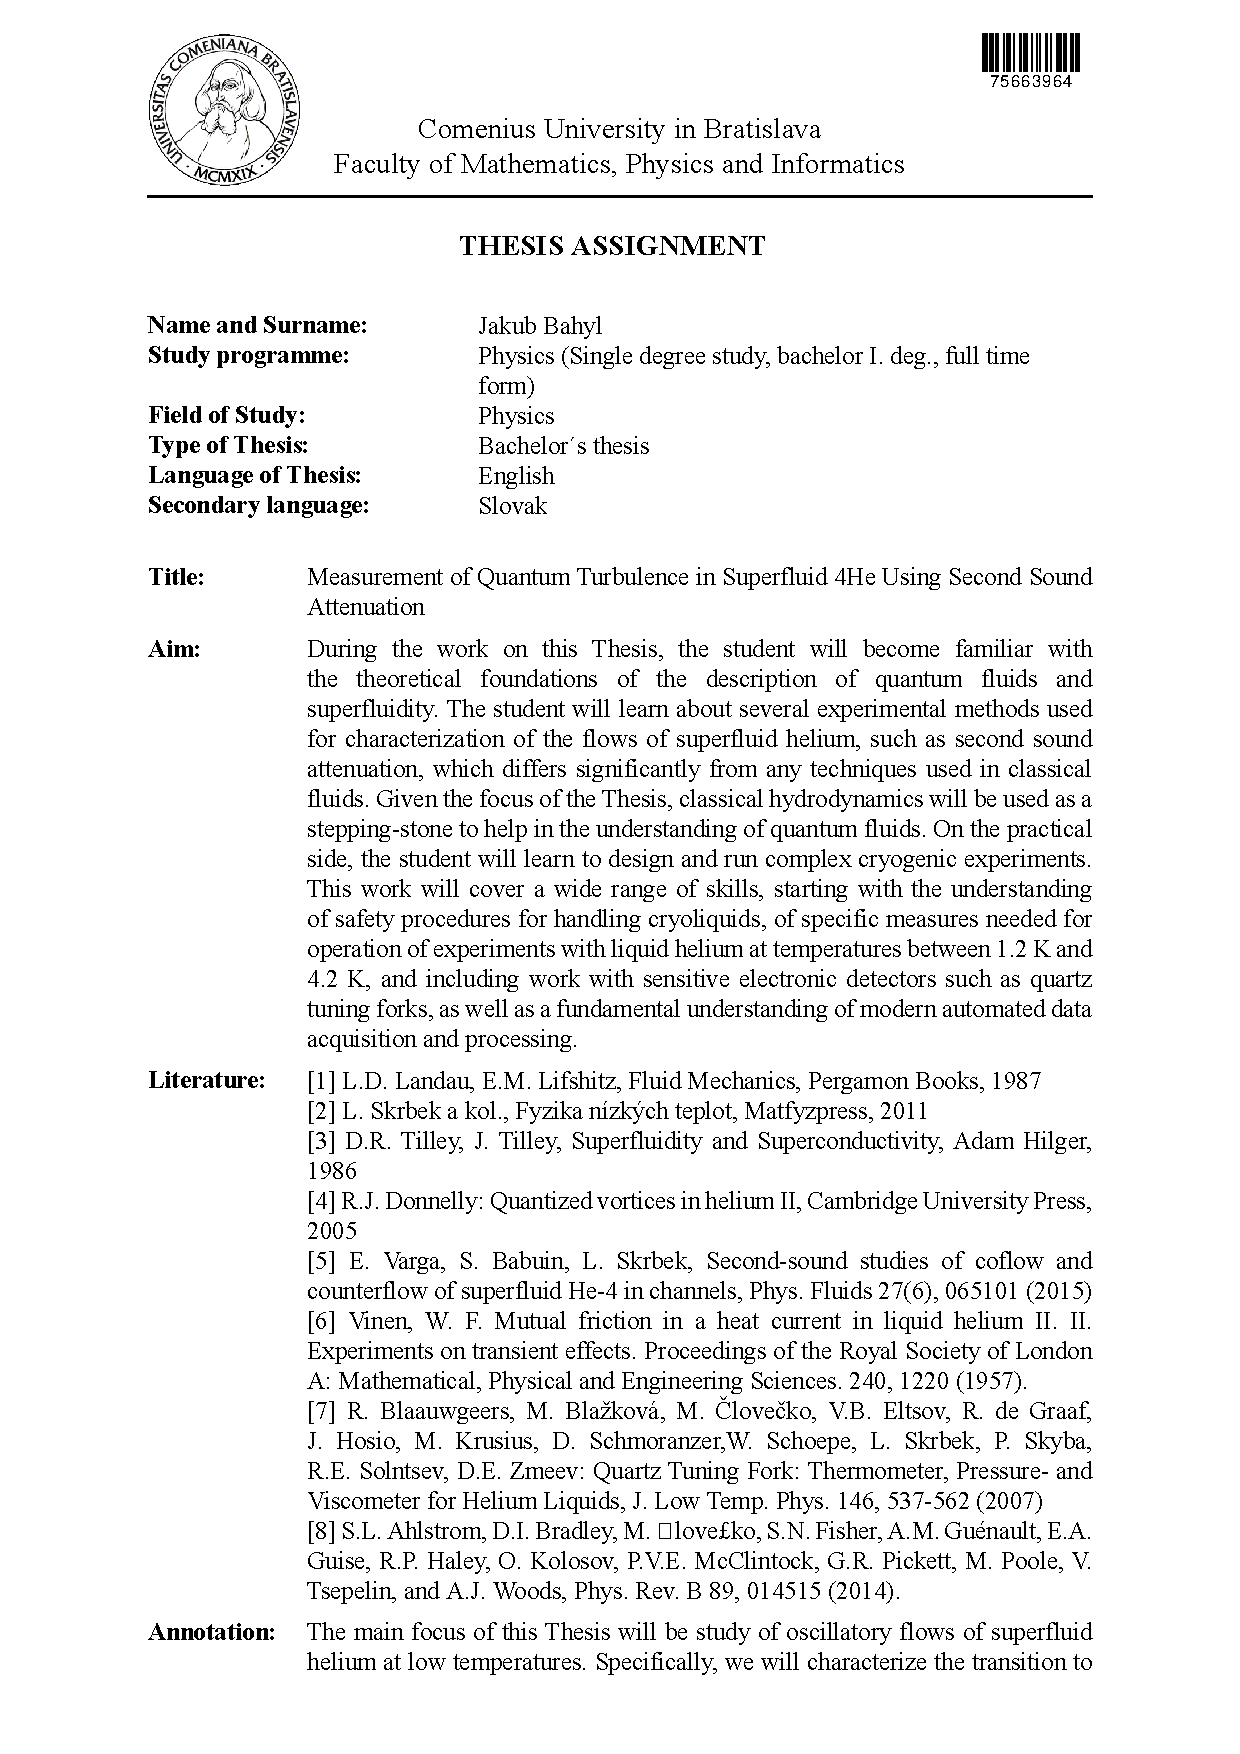
\includegraphics[width=0.9\textwidth]{docs/zadanie_Bahyl_EN.pdf}
% \newpage
%
% % Formal SVK
% 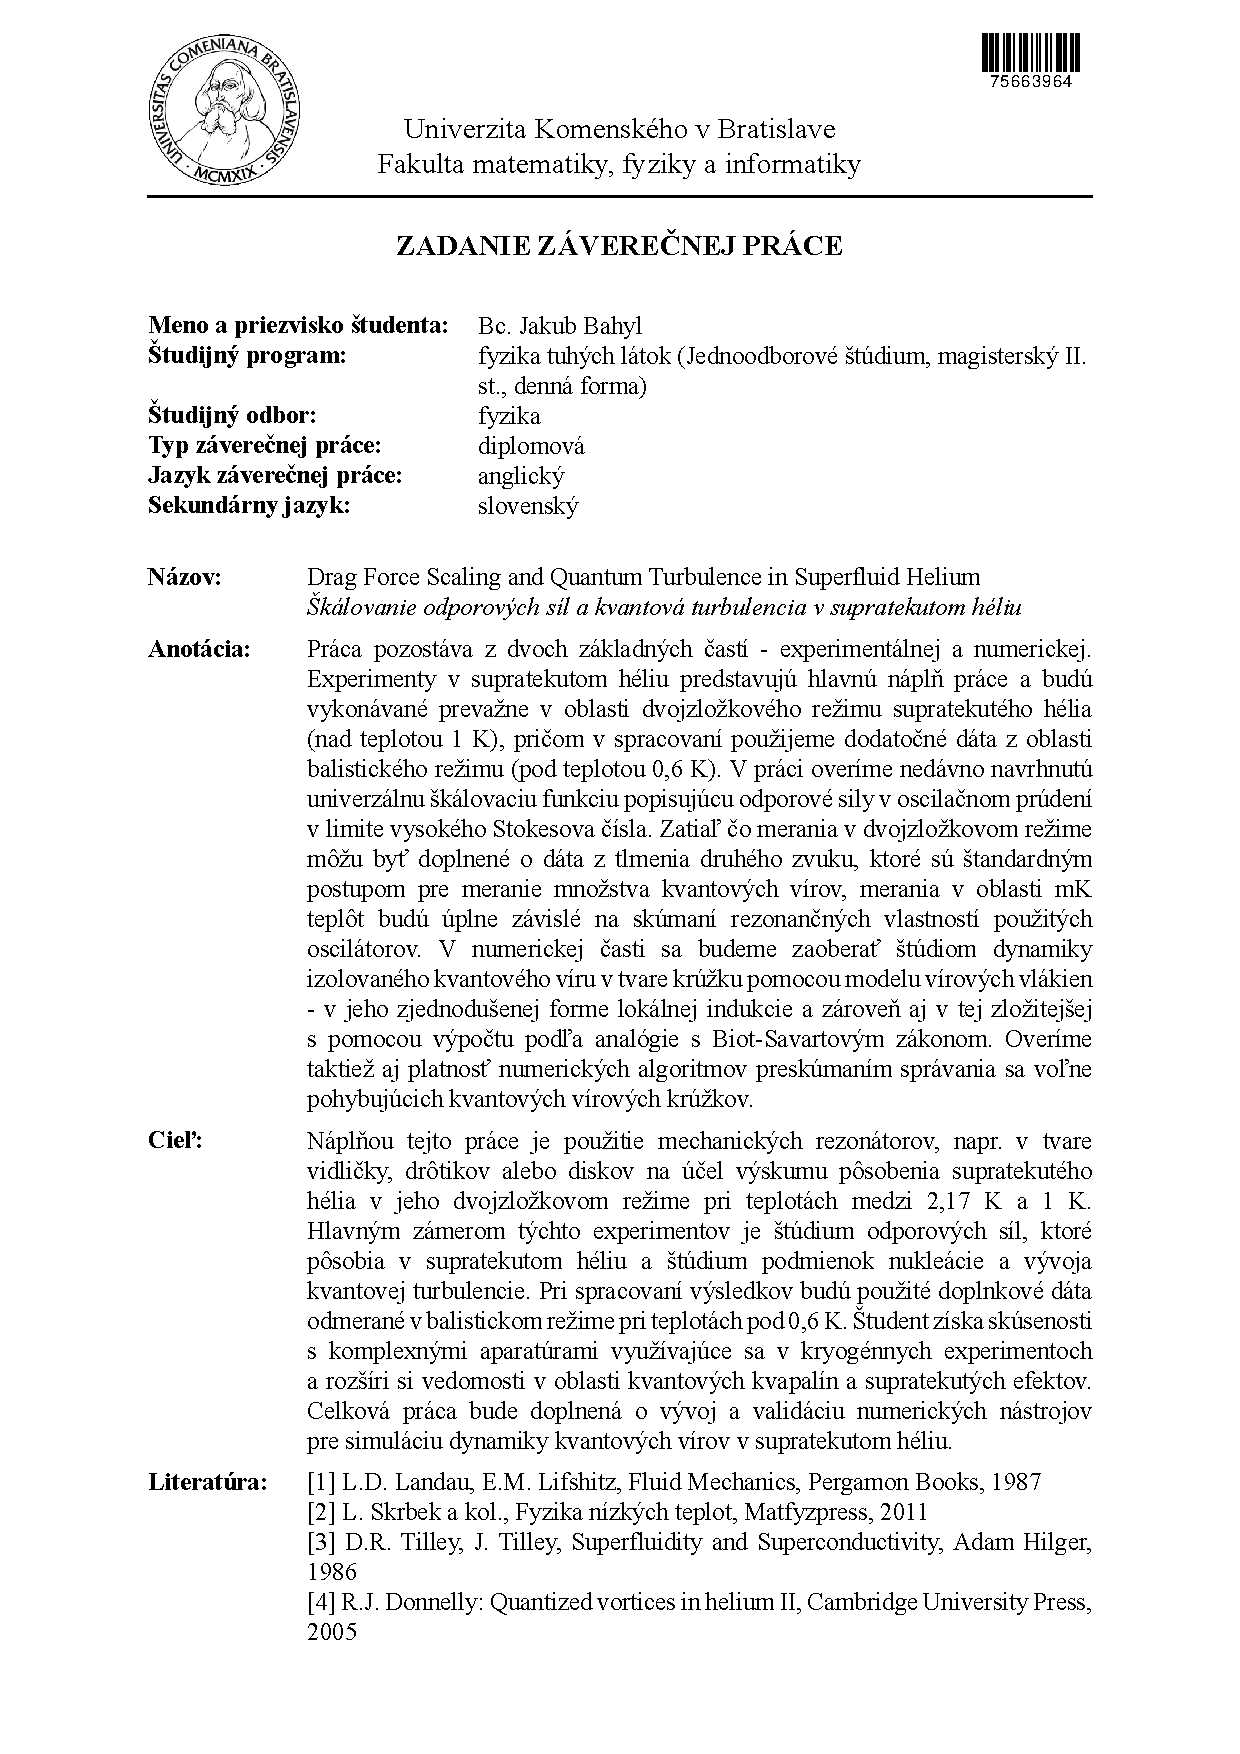
\includegraphics[width=0.9\textwidth]{docs/zadanie_Bahyl_SVK.pdf}
% \newpage
%
% % Acnkowledgements
% \chapter*{Acknowledgment}
\pagenumbering{gobble}

BACHELOR:
My special thanks go to my supervisor, David Schmoranzer, who gave me a  lot of experiences, knowledge and much more of his time, without which I definitely could not write this Thesis. Together with consultant Martin Jackson, they guided me during the whole experiment and helped me to understand all the important aspects included in this work. Moreover, I am thankful to Ladislav Skrbek and Patrik Švančara for giving me such a great opportunity to find out how astounding the experimental physics can be and to work with Superfluidity group within Charles University in Prague.

In the end, I would like to hugely thank my friends and family for all their \textit{„Good luck"} and \textit{„Keep going"} motivational quotes and other sort of supports, which I deeply appreciated.

DIPLOMA:
Thanks.
\todo{}

\vglue 0pt plus 1fill

\noindent
I declare that I carried out this master thesis independently, and only with the cited
sources, literature and other professional sources.


\vspace{10mm}

\hbox{
	\hbox to 0.5\hsize{%
		In \parbox[b]{2.5cm}{\dotfill}
		date \parbox[b]{2.5cm}{\dotfill}
	\hss}
	\hbox to 0.5\hsize{%
		Signature of the author:
		\hss}
	}

\newpage
%
% % Summary
% \vbox to \vsize{
\setlength\parskip{5mm}

{\bfseries \sffamily Názov práce}\\
Kvantová turbulencia v supratekutom héliu v teplotnej limite absolútnej nuly

{\bfseries \sffamily Autor}\\
Jakub Bahyl

{\bfseries \sffamily Školiteľ bakalárskej práce}\\
RNDr. David Schmoranzer, Ph.D.

{\bfseries \sffamily Abstrakt}\\
V tejto práci prezentujeme meranie kvantovej turbulencie generovanej oscilujúcim $ 6.5\unit{kHz} $ kremenným oscilátorom, ponoreným v supratekutom $ \He $ pri viacerých teplotách pod kritickou $ T_{\lambda} = 2.17\unit{K} $. Pozorovaná nelineárna odporová sila pôsobiaca na oscilátor je kvalitatívne spôsobená prítomnosťou klasickej turbulencie a kvantovaných vírov. Odporové sily a množstvo vytvorených kvantovaných vírov (hustota vírov čiar $ L $) sú nepriamo určené z útlmu druhého zvuku a mechanicko-elektrických vlastností oscilátora.
Výsledky, ktoré prezentujeme, kvantitatívne charakterizujú tvorbu klasickej aj kvantovej turbulencie. Ako prví ukazujeme, že obidve turbulencie vedia vzniknúť samostatne a nezávisle. Tento fakt je prezentovaný, v prvom priblížení, pomocou \textit{prúdového fázového diagramu}, v ktorom pre danú teplotu vieme predpokladať, kedy a ktorá turbulencia vzniká.

{\bfseries \sffamily Kľúčové slová}\\
supratekutosť $ \He $ $\bullet$ kvantový vír a turbulencia

\noindent\rule{16cm}{0.5pt}

{\bfseries \sffamily Title}\\
Quantum turbulence in superfluid helium down to the zero temperature limit

{\bfseries \sffamily Author}\\
Jakub Bahyl

{\bfseries \sffamily Supervisor}\\
RNDr. David Schmoranzer, Ph.D.

{\bfseries \sffamily Abstract}\\
In this Thesis, mechanical resonators such as \textit{tuning forks, wires are discs} are used to probe superfluid helium in the two-fluid regime at temperatures between temperatures $1.0\unit{K} < T < 2.17\unit{K}$. The principal aim of the experimental part is to study the drag forces arising from the superfluid and the nucleation and development of quantum turbulence. The obtained data, also with those from the ballistic regime $ T < 0.6\unit{K}$, are used to test a proposed \textit{Universal scaling relation} describing the drag forces in high-Stokes-number oscillatory flow.\\
The experimental work is complemented by developing and validating the tools necessary for numerical simulations of quantized vortex dynamics in superfluid helium. In this part, dynamics of a single quantized vortex ring are studied using the \textit{Vortex filament model}.


{\bfseries \sffamily Keywords}\\
superfluidity of $ \He $  $\bullet$ quantum vortex and turbulence

\vss}

\newpage
% \newpage

%%%%%%%%%%%%%%%%%%%%%%%%%%%%%%%%%%%%%%%%%%%%%%%%%%%%%%%%%%%%%%%%%%%%%%%%%%%%%%
%% THESIS
%%%%%%%%%%%%%%%%%%%%%%%%%%%%%%%%%%%%%%%%%%%%%%%%%%%%%%%%%%%%%%%%%%%%%%%%%%%%%%

\pagenumbering{arabic}
\pagestyle{plain}
\setcounter{page}{1}
\spacing{1.2}

% Content
\tableofcontents

% Chapters
\chapter*{Introduction}
\addcontentsline{toc}{chapter}{Introduction}

	To this day, turbulent motion of fluids remains the last unresolved problem of classical physics. They present many practical challenges across different areas of industry (f.e. weather prediction). Quantum turbulence, in contrast, may occur only in superfluids and was first observed in superfluid state of $\He$. Compared to classical turbulence, it can be regarded as a simpler system from the theoretical and numerical point of view. Also, it shares many of the general properties of turbulence in classical viscous fluids.

	In very low temperatures, the liquid state of $\He$ exists in two phases:
	\begin{itemize}
		\item \underline{Helium-I}: a high temperature phase ($2.17\unit{K}<T<4.2\unit{K}$)
		\item \underline{Helium-II}: a low temperature phase ($T<2.17\unit{K}$)
	\end{itemize}

	These two phases are connected with the \textit{lambda transition}, which occurs at the critical temperature $T_{\lambda} = 2.17 \unit{K}$ at saturated vapour pressure (\textbf{Figure \ref{phase_diag}}). Helium-I is a classical fluid described by ordinary Navier-Stokes (N-S) equations, whereas Helium-II is a superfluid and behaves partly like a Bose-Einstein condensate.

	\begin{figure}[h]
		\centering
		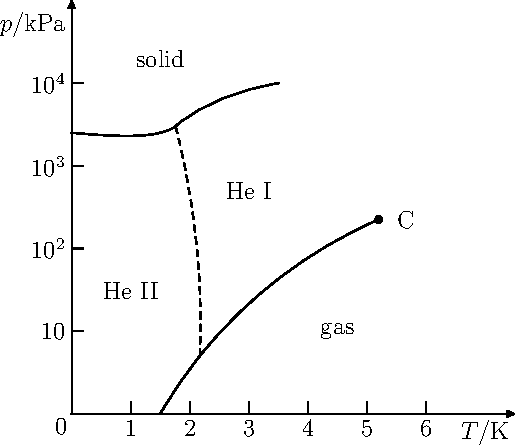
\includegraphics[width=0.6\textwidth]{graphics/theory/phase_diag}
		\caption{Pressure-Temperature diagram of $\He$. Fixing pressure on an atmospheric value, a gas-liquid transition is present at $4.2\unit{K}$ (He-I) and a superfluid transition at $2.17\unit{K}$.}
		\label{phase_diag}
	\end{figure}

	A simple, phenomenological model of the Helium-II motion was proposed by Tisza \cite{tisza} and Landau \cite{landau} - the \textit{two-fluid model}. According to two-fluid model, it behaves as if composed of two inter-penetrating liquids - the normal and superfluid components - with corresponding velocity fields and temperature-dependent densities:

	\begin{itemize}
		\item \underline{normal component}: density $\rho_n (T)$, velocity field $\vec{v}_n (\vec{r}, t)$, motion described by an ordinary viscous Navier-Stokes equation, carrying entropy and represented as a collection of thermal excitations such as \textit{phonons} and \textit{rotons}
		\item \underline{superfluid component}: density $\rho_s (T)$, velocity field $\vec{v}_s(\vec{r}, t)$, motion described by a modified Euler equation (without viscosity) with quantum terms, no entropy and represented by a macroscopic wave function
	\end{itemize}

	The total density of Helium-II sums up to $\rho = \rho_n(T) + \rho_s(T) \approx \text{const}$ and the relative proportion of normal/superfluid component is determined mainly by the temperature (\textbf{Figure \ref{densities}}). Near $T \rightarrow 0$ Helium-II becomes entirely superfluid $\rho_s/\rho \rightarrow 1$. The temperature dependence of this ratio is highly nonlinear. For example, the ratio $\rho_n/\rho$ drops from $100\%$ at $2.17\unit{K}$ to $50\%$ at $1.95\unit{K}$, to $<5\%$ at $1.3\unit{K}$, and is effectively negligible under $1\unit{K}$.

	\begin{figure}[h]
		\centering
		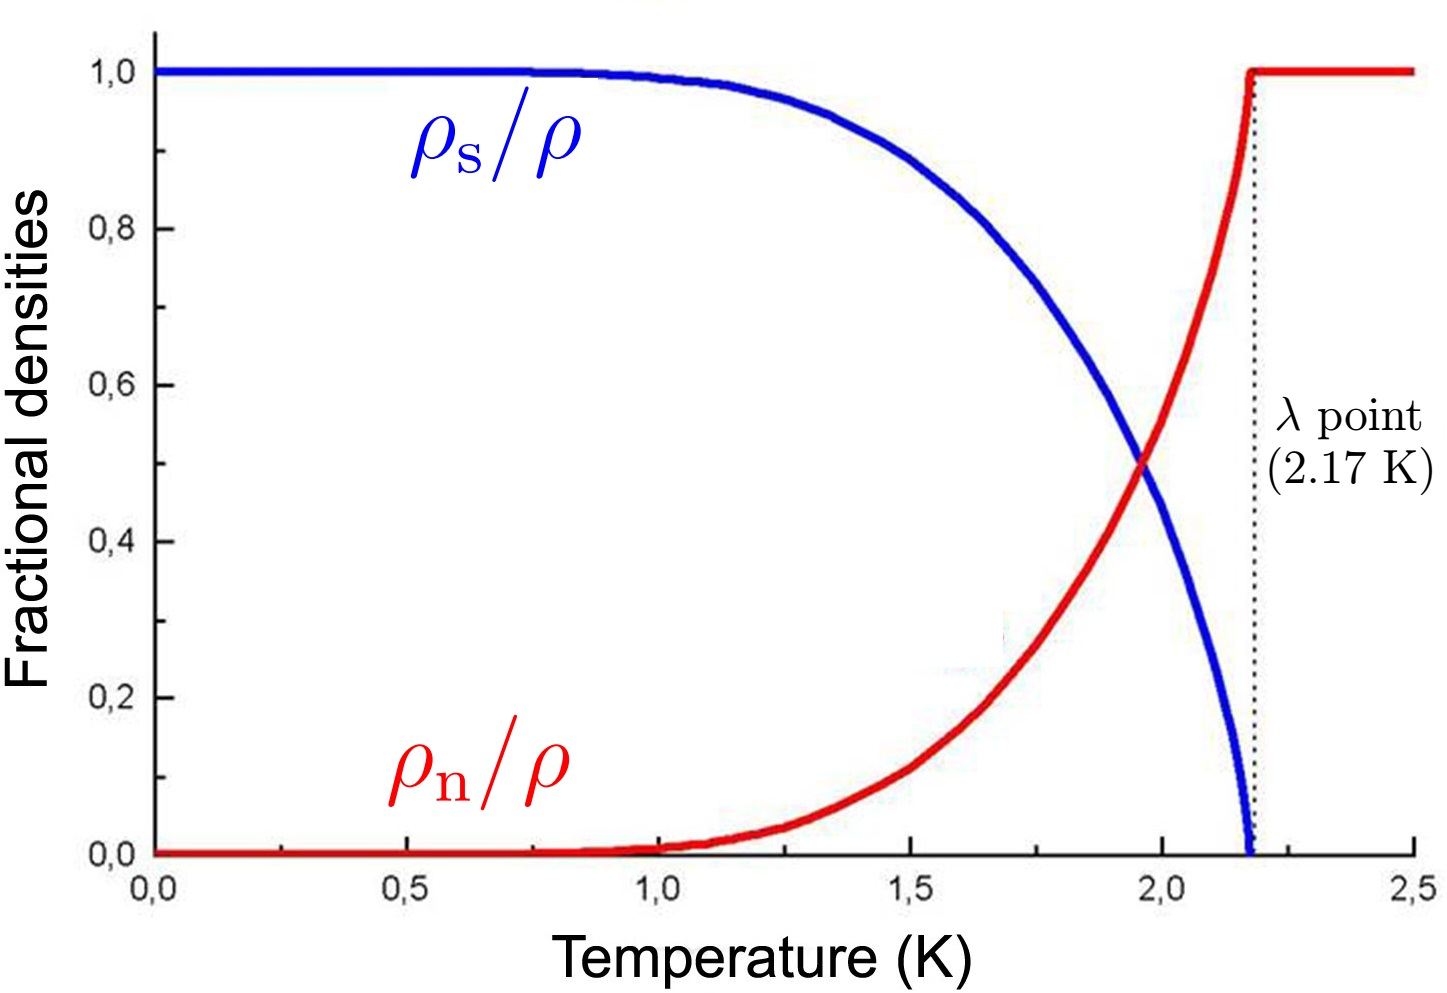
\includegraphics[width=0.6\textwidth]{graphics/theory/densities}
		\caption{Temperature dependence of fractional densities of the normal (red) and superfluid (blue) components. Source: \cite{svoc2016}}
		\label{densities}
	\end{figure}

	It arises from the quantum nature of superfluid, that the superfluid component should not perform any rotation. However, when this component moves faster than a critical velocity, the circulation is \textit{quantized} and so-called \textit{quantized vortices} are created, which makes the hydrodynamics of Helium-II particularly interesting. The vortex nucleation process is still a subject of many current investigations. Superfluid vortex lines were observed spatially organized, but also completely disorganized as simulated in \textbf{Figure \ref{sim_cube}}. Quantum turbulence therefore takes the form of a tangle of quantized vortices in the superfluid component which typically coexist with classical turbulent flow of the normal component.

	In the presence of quantized vortices, the independent normal and superfluid velocity fields become coupled by the \textit{mutual friction} force which arises due to quasiparticles scattering off the cores of vortices.

	\begin{figure}[h]
		\centering
		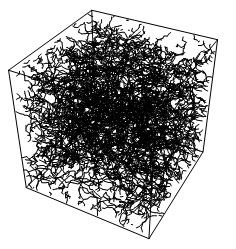
\includegraphics[width=0.4\textwidth]{graphics/theory/QT-tangle}
		\caption{Cube of numerically simulated tangle of randomly distributed quantised vortices. Source: \cite{svoc2016}}
		\label{sim_cube}
	\end{figure}

	Also we note that for a typical experiment, below $\sim 0.7\unit{K}$, a transition to ballistic regime occurs in the normal component, as the mean free path of phonons exceeds the characteristic dimensions of the experimental setup. This situation is similar to the one of dilute classical gases.

	Quantum turbulence can be experimentally achieved in many traditional ways - driving a mass flow, spinning discs, oscillating grids and forks, ultrasound and jets.\\
	To characterize the turbulence one may use a superfluid Reynolds number for a steady flows, or a newly introduced \cite{universal_scaling} Donnelly number for high-frequency oscillatory flows.
	We find that for quantum turbulence originated in high-frequency regime above temperature $T > 1\unit{K}$, the measured drag forces are described in terms of a single dimensionless parameter and exhibit an universal scaling behaviour. We identify and compare the critical conditions related to the production of both quantized vorticity and instabilities occuring in normal component.

	Besides experimental approaches on quantum fluids, one of the useful tools for understanding the geometry and flow of quantum turbulence, is the \textit{vortex filament model}, pioneered by Schwarz \cite{schwarz}. With the rapid development of available computational power, large simulations have become the methods of choice for calculating the motion of fluids. In superfluids like Helium-II, due to the quantization of circulation, vorticity can only exist within vortex filaments with a certain core size, which makes the model highly applicable.

	We propose an efficient numerical method to compute the time evolution of vortex filaments in superfluid Helium-II. We studied the performance and stability and well replicated the physical processes such as the annihilation of quantized vortex rings \cite{vortex_ring} while travelling across superfluid.\\
	We also present the \texttt{PyVort} code, a new platform in Python 3 to simulate quantized rings phenomena. More on the implementation part can be found in \textbf{Simulation} and \textbf{Appendix}.

%%%%%%%%%%%%%%%%%%%%%%%%%%%%%%%%%%%%%%%%%%%%%%%%%%%%%%%%%%%%%%%%%%%%%%%%%%%%%%

	\section*{Motivations and Goals}

	Here we briefly collect all motivations and goals that led us to our investigations.

	\subsection*{Experimental approach}

	\begin{itemize}
		\item ivestigate transition from laminar and potential flow of normal and superlfuid components, respectively, to classical or quantum turbulence at various temperatures above $>1\unit{K}$ in high-frequency regime.
		\item construct an experiment using flow generators such as vibrating wire, tuning fork and oscillating disc and observe the drag phenomena
		\item apply universal scaling theory and prove the concept on collected experimental data
	\end{itemize}

	\subsection*{Simulation}
	\begin{itemize}
		\item build modular and reusable codebase in Python 3 that simulates the dynamics of quantized vortices using the \textit{Vortex Filament} model
		\item implement stable time-step methods and a reliable re-segmentation process that allows keeping a good resolution of quantized vortices in different situations
		\item simulate a real-time quantum vortex ring motion and compare its properties and evolution in time with the theoretical approaches, thus validating the new codebase
	\end{itemize}

\newpage

%%%%%%%%%%%%%%%%%%%%%%%%%%%%%%%%%%%%%%%%%%%%%%%%%%%%%%%%%%%%%%%%%%%%%%%%%%%%%%
%%%%%%%%%%%%%%%%%%%%%%%%%%%%%%%%%%%%%%%%%%%%%%%%%%%%%%%%%%%%%%%%%%%%%%%%%%%%%%
%%%%%%%%%%%%%%%%%%%%%%%%%%%%%%%%%%%%%%%%%%%%%%%%%%%%%%%%%%%%%%%%%%%%%%%%%%%%%%

\chapter{Theoretical Background}

The theoretical part of this Thesis is composed of two chapters:

\begin{itemize}
	\item[1.] \underline{Micro/Meso-scopic view} - provides a theoretical cover of Gross-Pitaevskii model, creation and numerical modelling of the quantized vortex and its dynamics.

	\item[3.] \underline{Macroscopic view} - provides a hydrodynamics description of two-fluid model, oscillatory motion in He-II, creation of quantum turbulence, dynamical and universal scaling principles

\end{itemize}

The aim of the theoretical part is to introduce the basic properties of quantized vortex lines in Helium-II and summarize the state of art of current knowledge on superfluid turbulence. We also discuss the theoretical methods used to study quantized vorticity, quantum turbulence and the results obtained using such methods.

%%%%%%%%%%%%%%%%%%%%%%%%%%%%%%%%%%%%%%%%%%%%%%%%%%%%%%%%%%%%%%%%%%%%%%%%%%%%%%
%%%%%%%%%%%%%%%%%%%%%%%%%%%%%%%%%%%%%%%%%%%%%%%%%%%%%%%%%%%%%%%%%%%%%%%%%%%%%%

\newpage

{\Huge \bfseries Micro/Meso-scopic view}
\addcontentsline{toc}{chapter}{Micro/Meso-scopic model}
\vspace{0.3cm}

One of the most useful ways of describing superfluid $\He$ at $T=0\unit{K}$ starts with nonlinear Schrodinger equation (NLSE) for the one-particle wave function $\psi$. Since the superfluid $\He$ is a strongly correlated system dominated by collective effects, this imperfect Bose-Einstein condensate (BEC) is approximately described by Gross-Pitaevskii equation (\ref{gross-pit}). Although, it must be noted that the real Helium-II is a dense fluid, not a weakly interacting Bose gas described by NLSE.

%%%%%%%%%%%%%%%%%%%%%%%%%%%%%%%%%%%%%%%%%%%%%%%%%%%%%%%%%%%%%%%%%%%%%%%%%%%%%%

\section{Gross-Pitaevskii model}

In terms of single-particle wavefunction $\psi(\vec{r},t)$ we write the Gross-Pitaevskii model:

\begin{equation}
i \hbar \frac{\partial \psi}{\partial t} = - \frac{\hbar^2}{2m} \nabla^2 \psi
+ \psi \int \vert \psi(\vec{r}^{\prime},t) \vert^2 V(\vert \vec{r} - \vec{r}^{\prime} \vert)
\text{d}\vec{r}^{\prime}\,,
\label{gross-pit}
\end{equation}

where $V(\vert \vec{r} - \vec{r}^{\prime} \vert)$ is the potential of two-body interaction between bosons. The normalization is set as $\int \vert \psi \vert^2 \text{d}\vec{r} = N$, where $N$ is number of bosons. By replacing potential with repulsive $\delta$-function of strength $V_0$ one obtains:

\begin{equation}
i \hbar \frac{\partial \Psi}{\partial t} = - \frac{\hbar^2}{2m} \nabla^2 \Psi - m\eps \Psi + V_0 \vert \Psi \vert^2 \Psi\,,
\label{GP}
\end{equation}

where $\eps$ is the energy per unit mass and $\Psi = A e^{i\Phi}$ is a macroscopic wave function of condensate. In this way one can define the condensate's density $\rho_{BEC} = m\Psi\Psi^* =  mA^2$ and velocity $\vec{v}_{BEC} = (\hbar / m)\nabla \Psi$. Note that equation (\ref{GP}) is equivalent to a continuity equation and an modified Euler equation (by the so called quantum pressure term).

Hereafter we identify $\rho_{BEC}$ with $\He$ superfluid component's $\rho_s$ at absolute zero and $\vec{v}_{BEC}$ with $\vec{v}_s$. It must be noted that this identification is convenient from the point of view of having a simple hydrodynamics model but is not entirely correct. The reason is
that Helium-II is a dense fluid, not the weakly interacting Bose gas described
by the NLSE (\ref{gross-pit}), so the condensate is not the same as the superfluid component.

\newpage

Even though the superfluid is irrotational: $\omega = \nabla \times \vec{v}_s = \vec{0}$, the NLSE has a vortex-like solution: $\vec{v}_s = \varkappa / 2\pi r\, \vec{e_{\theta}}$, where $\theta$ is the azimuthal angle and $\varkappa=9.97 \times 10^{-4} \unit{cm^2 \dotprod s^{-1}}$ is the \textit{quantum of circulation}, obtained from:

\begin{equation}
\varkappa = \oint_{\mathcal{C}} \vec{v}_{BEC} \cdot \unit{d}\vec{\boldsymbol{\ell}} = \frac{h}{m}\,,
\label{varkappa}
\end{equation}

where $\mathcal{C}$ is a closed loop surrounding the vortex core - a topological defect (\textbf{Figure {\ref{singularity}}}) within macroscopic wavefunction $\Psi$

\begin{figure}[h]
	\centering
	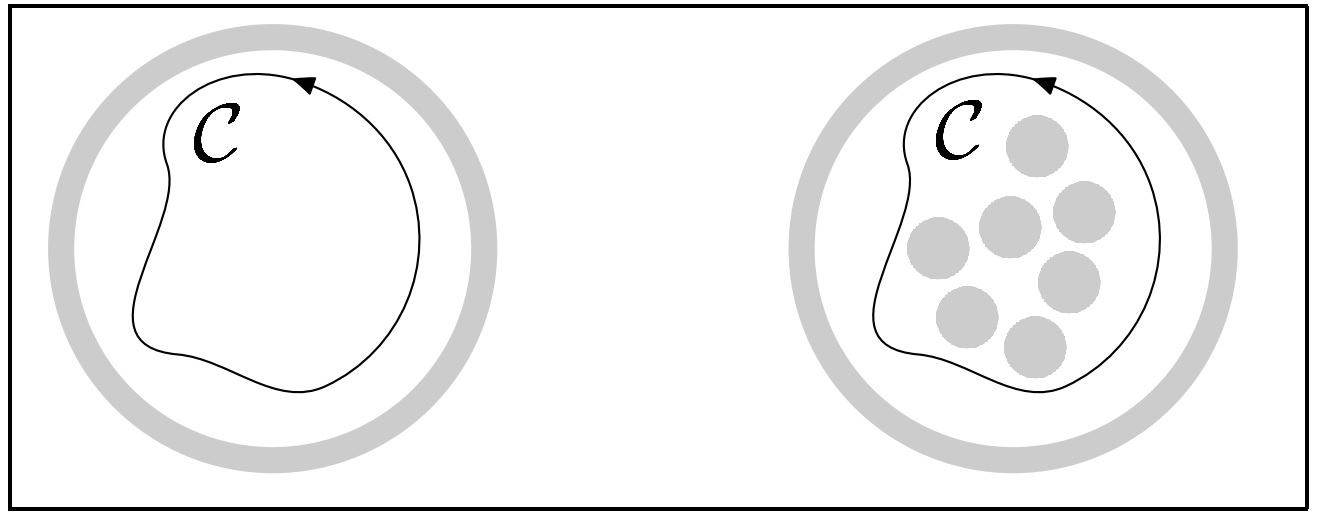
\includegraphics[width=0.6\textwidth]{graphics/theory/singularity}
	\caption{An illustration of topological singularities within a superfluid $\He$. Left: A singly-connected irrotational region with circulation along $\mathcal{C}$ loop equal to zero. Right: A multiply-connected region with depicted cores of quantized vortices with a finite circulation along $\mathcal{C}$ loop.}
	\label{singularity}
\end{figure}

%%%%%%%%%%%%%%%%%%%%%%%%%%%%%%%%%%%%%%%%%%%%%%%%%%%%%%%%%%%%%%%%%%%%%%%%%%%%%%

\section{Quantized vortex}

As Feynman showed \cite{feynman}, superfluid vortex lines appear when Helium-II moves faster than a certain critical velocity. The simplest way to create quantum vortices is to rotate cylinder with superfluid Helium-II with high enough angular velocity $\Omega$. Created vortex lines form an ordered array of density $L=2\Omega / \varkappa$, all aligned along the axis of rotation (\textbf{Figure \ref{rotating-helium}}). \textit{Vortex line density} $L$ can be also interpreted as a total vortex length in an unit volume.

\begin{figure}[h]
	\centering
	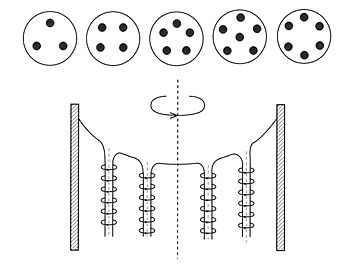
\includegraphics[width=0.4\textwidth]{graphics/theory/rotating-helium}
	\caption{Array of quantized vortices in a rotating container}
	\label{rotating-helium}
\end{figure}

The key properties of Onsager-Feynman vortex \cite{onsager} are the quantized circulation $\varkappa$, superfluid rotational velocity field $\vec{v}_s = \varkappa / 2\pi r\, \vec{e_{\theta}}$ and the \textit{vortex core parameter} $a_0$. The core size $a_0$ can be estimated by substituting $\vec{v}_s$ back into (\ref{GP}) and solving differential equation for $\rho_s$. One finds that $\rho_s$ tends to the value $m^2 \eps / V_0$ for $r \rightarrow \infty$ and to zero density for $r \rightarrow 0$.
The characteristic distance over which $\Psi$ collapses (superfluid density $\rho_s$ drops from bulk value to zero) is $a_0 \approx 10^{-10} \unit{m} = 1 \unit{\AA}$. From this, there is a conclusion that the vortex is hollow at its core and therefore, a topological defect occurs.

Taking $a_0$ as core radius, the energy considerations showed that a single vortex containing $N$ circulation quanta owns more energy than $N$ singly-quantized vortices. Hence it is generally assumed that only ground-state vortices are commonly observed.

Clearly, vortex lines don't have to be aligned in general. In most cases , the superfluid flow is strongly chaotic, better known as \textit{quantum turbulence}. This topic is covered in more detail later in this work.

%%%%%%%%%%%%%%%%%%%%%%%%%%%%%%%%%%%%%%%%%%%%%%%%%%%%%%%%%%%%%%%%%%%%%%%%%%%%%%

\section{Vortex filament model}

The vortex line can be represented as a curve via position vector $\vec{s} = \vec{s}(\xi, t)$ in three-dimensional space. Here, $\xi$ is arclength along the vortex line. Next we label $\vec{s}^{\prime}$ as $\text{d}\vec{s} / \text{d} \xi$ and $\vec{s}^{\prime\prime}$ as $\text{d}\vec{s}^{\prime} / \text{d} \xi$.
Within our context, $\vec{s}^{\prime}$ is a tangent vector and $\vert \vec{s}^{\prime\prime} \vert$ is a local curvature $R^{-1}$ at a given point.
The triad of vectors $\vec{s}^{\prime}$, $\vec{s}^{\prime\prime}$, $\vec{s}^{\prime} \times \vec{s}^{\prime\prime}$ are perpendicular to each other (\textbf{Figure \ref{filament}}) and point along the tangent, normal and binormal respectively:

\begin{figure}[h]
	\centering
	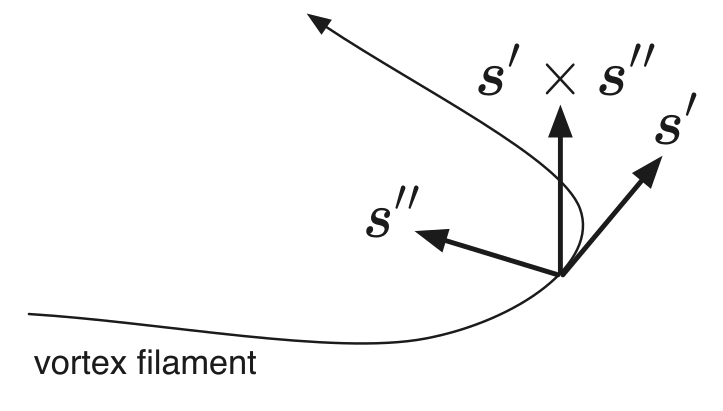
\includegraphics[width=0.7\textwidth]{graphics/theory/filament}
	\caption{Schematic of the vortex filament and the triad vectors $\vec{s}^{\prime}$, $\vec{s}^{\prime\prime}$, $\vec{s}^{\prime} \times \vec{s}^{\prime\prime}$. Source: \cite{tsubota}}
	\label{filament}
\end{figure}

We suppose that the superfluid component is incompressible $\nabla \dotprod \vec{v}_s = 0$. Moreover, superfluid vorticity $\omega_s$ is localized only at positions of vortex filament $\omega_s(\vec{r},t) = \nabla \times \vec{v}_s$. Combining these two properties gives the Poisson equation $\Delta \phi = \omega_s$ for the potential $\phi$.
Using Fourier transform one obtains \cite{barenghi} the Biot-Savart law for the superfluid velocity:

\begin{equation}
\vec{v}_s(\vec{r}) = \frac{\varkappa}{4\pi} \int_{\mathcal{L}} \frac{(\vec{r^{\prime}} - \vec{r}) \times \text{d}\vec{r^{\prime}}}{\vert \vec{r^{\prime}} - \vec{r} \vert^3}\,,
\label{biot_general}
\end{equation}

where the integral path $\mathcal{L}$ represents curves along all vortex filaments.

This law determines the superfluid velocity field $\vec{v}_s(\vec{r})$ via the arrangement of the vortex filaments. Now we define the \textit{self-induced} velocity $\vec{v}_{\text{ind}}$, describing the motion which a vortex line induces onto itself ($\vec{r} \rightarrow \vec{s}$ in (\ref{biot_general})) due to its own curvatures:

\begin{equation}
\vec{v}_{\text{ind}}(\vec{s}) = \frac{\varkappa}{4\pi} \int_{\mathcal{L}} \frac{(\vec{r^{\prime}} - \vec{s}) \times \text{d}\vec{r^{\prime}}}{\vert \vec{r^{\prime}} - \vec{s} \vert^3}
\label{biot_ind}
\end{equation}

However, this integral (\ref{biot_ind}) diverges as $\vec{r}^{\prime} \rightarrow \vec{s}$ because the core structure
of the quantized vortex was initially neglected. We avoid this divergence by splitting the integral into two parts - direct neighbourhood of the point $\vec{s}$ (local part) and the rest $\mathcal{L}^{\prime}$ (nonlocal part). The Taylor expansion of the local part leads \cite{schwarz} to a finite result:

\begin{align}
\vec{v}_{\text{ind}}(\vec{s})
= \vec{v}_{\text{ind,local}} + \vec{v}_{\text{ind,nonlocal}}
\approx& \beta \vec{s}^{\prime} \times \vec{s}^{\prime \prime} + \frac{\varkappa}{4\pi} \int_{\mathcal{L}^{\prime}} \frac{(\vec{r^{\prime}} - \vec{s}) \times \text{d}\vec{r^{\prime}}}{\vert \vec{r^{\prime}} - \vec{s} \vert^3}\,,
\label{lia+biot}
\\
\text{where}\, \beta =& \frac{\varkappa}{4\pi} \ln(R / a_0)\,,
\label{beta}
\end{align}

where $\mathcal{L}^{\prime}$ is the original vortex line without a close area of the studied vortex point and $R$ is a \textit{local curvature} and often is calculated as $1 / \vert \vec{s}^{\prime\prime} \vert$ \cite{schwarz}.

Since the local part of induced velocity (\ref{lia+biot}) is a dominant term (and also computationally faster), the nonlocal part can be neglected. Such approximation process is called as \textit{Local Induction Approximation} (LIA). LIA represents the contribution of local curvature to the induced velocity, whereas nonlocal Biot-Savart part represents the global filament curvature.

Since in the system there could be present also external flow sources of superfluid component (e.g. heat resistors causing \textit{counterflows}), we define the total superfluid velocity $\vec{v}_{s,tot}$, in a laboratory frame, as:

\begin{equation}
\vec{v}_{s,tot} = \vec{v}_{s,ext} + \vec{v}_{\text{ind}}
\end{equation}

\newpage

%%%%%%%%%%%%%%%%%%%%%%%%%%%%%%%%%%%%%%%%%%%%%%%%%%%%%%%%%%%%%%%%%%%%%%%%%%%%%%


\section{Vortex dynamics}

To determine the equation of motion of $\vec{s}(t)$ we recognize the forces acting upon the line - the magnus force $\vec{f}_M$ and (at non-zero temparature $T>0\unit{K}$ )the drag force $\vec{f}_D$ (both are per unit length).

The magnus force $\vec{f}_M$ always arises when a rotating body moves in a flow. This causes a pressure difference, which in our case of moving vortex line with circulation quantum $\varkappa$, exerts a force:

\begin{equation}
\vec{f}_M = \rho_s \varkappa \,\vec{s}^{\prime} \times (\vec{\dot{s}} - \vec{v}_{s,tot})\,,
\label{magnus}
\end{equation}

where $\vec{\dot{s}} = \text{d}\vec{s} / \text{d} t$ is the velocity of a particular point on a vortex line.

The drag force $\vec{f}_D$ arises from the \textit{mutual friction}, the interaction between the normal component and vortex lines (quantized superfluid component). According to the findings of Vinen and Hall \cite{vinen}, the normal fluid flowing with velocity $\vec{v}_n$ past a vortex core exerts a frictional force $\vec{f}_D$ on the vortex line, given by:

\begin{align}
\vec{f}_D = -& \alpha(T)\rho_s\varkappa\,\vec{s}^{\prime} \times [\vec{s}^{\prime} \times (\vec{v}_{ns} - \vec{v}_{\text{ind}})]
\label{alpha1}
\\
-& \alpha^{\prime}(T)\rho_s\varkappa\,\vec{s}^{\prime} \times (\vec{v}_{ns} - \vec{v}_{\text{ind}})
\,,
\label{alpha2}
\end{align}

where $\vec{v}_{ns} = \vec{v}_{n} - \vec{v}_{s,ext}$ is the difference between the average velocity of normal component and the applied superfluid velocity.

The temperature dependent dimensionless parameters $\alpha(T)$ and $\alpha^{\prime}(T)$ are often written in terms of measured \textit{mutual friction parameters} $B$ and $B^{\prime}$, which are known from experiments by Samuels and Donnelly \cite{donnelly}:

\begin{equation}
\alpha(T) = \frac{\rho_n B(T)}{2\rho}
\hspace{1cm}
\alpha^{\prime}(T) = \frac{\rho_n B^{\prime}(T)}{2\rho}
\end{equation}

The precise calculation of the mutual friction parameters $B(T), B^{\prime}(T)$ over the entire temperature range is still an open problem. Although, we already know that in the area of high temperatures, the friction arises mainly from the scattering processes of rotons.

\newpage

Since the mass of vortex core is usually neglected, the two forces $\vec{f}_M$ and $\vec{f}_D$ add up to zero: $\vec{f}_M + \vec{f}_D = \vec{0}$. Hence, solving for $\text{d}\vec{s} / \text{d} t$, we obtain \cite{schwarz} the Schwarz's equation:

\begin{equation}
\dot{s} = \vec{v}_{\text{s, ext}} + \vec{v}_{\text{ind}}
+ \alpha\vec{s}^{\prime} \times (\vec{v}_{ns} - \vec{v}_{\text{ind}})
- \alpha^{\prime}\vec{s}^{\prime} \times [\vec{s}^{\prime} \times (\vec{v}_{ns} - \vec{v}_{\text{ind}})]\,,
\label{schwarz}
\end{equation}

On the basis of Schwarz's equation (\ref{schwarz}), algorithms to numerically simulate vortex time evolution of an arbitrary configuration can be developed. Also, the vortex parametrisation $\vec{s}(\xi, t)$ and dynamics description provide the baseline of what we call as Vortex Filament (VF) model. More on VF model is written later in \textbf{Simulation} chapter.

%%%%%%%%%%%%%%%%%%%%%%%%%%%%%%%%%%%%%%%%%%%%%%%%%%%%%%%%%%%%%%%%%%%%%%%%%%%%%%


\subsection*{Quantized vortex rings}

A special case of vortex line configuration are a freely moving vortex rings. Such rings are usually created as a result of multi-vortex interconnections \cite{vortex_ring} or by the self-reconnection of an oscillating loop pinned to the surface of a vibrating body. The exact expressions derived from the Gross-Pitaevskii equation (\ref{gross-pit}) \cite{roberts} for the energy $E$ and induced center velocity $v_{\text{ind}}$ of a vortex ring, moving in a Helium-II of density $\rho$ and having a radius $R$ much greater than its core radius $R >> a_0$, are:

\begin{equation}
E = \frac{1}{2}\varkappa^2 \rho R \Big(\ln(8R/a_0) - 2 + c\Big)
\label{ring-energy}
\end{equation}

\begin{equation}
v_{\text{ind}} = \frac{\varkappa}{4\pi R} \Big(\ln(8R/a_0) - 1 + c\Big)\,,
\label{ring-velocity}
\end{equation}

where $c$ is a constant based on inner structure of the vortex. Since we work with hollow core, we use \cite{donnelly_book}
$c = 1/2$. Note that (\ref{ring-energy}) and (\ref{ring-velocity}) depend on $a_0$ only logarithmically.
The behavior of the vortex ring is thus quite insensitive to the exact value of $a_0$ (expected to be of the order of atomic dimension).

Relations (\ref{ring-energy}) and (\ref{ring-velocity}) are derived directly from Gross-Pitaevskii description and no dissipative process (mutual friction) was included. Therefore, the relations hold only for temperature $T=0\unit{K}$, Using the explicit dynamical equation \cite{donnelly_book} for vortex ring motion, one can also derive the final ring center velocity $\vec{v}_{\text{ring}}$ and energy $E_{\text{ring}}$ using (\ref{ring-energy}) and (\ref{ring-velocity}) like:

\begin{equation}
\vec{v}_{\text{ring}} = (1 - \alpha^{\prime}) (\vec{v}_{\text{ind}} - \vec{v}_{\text{s, ext}})
+ \alpha^{\prime} \vec{v}_{\text{n, ext}}
\label{v_ring}
\end{equation}

\begin{equation}
E_{\text{ring}} = \Big( \frac{\alpha}{1 - \alpha^{\prime}} \Big) E
\label{E_ring}
\end{equation}

Several other interesting results come from the ring's dynamic motion equation and the mutual friction formula (\ref{alpha1}), (\ref{alpha2}). The second term (\ref{alpha2}) of friction force causes the decrease of vortex ring radius, whereas the first term (\ref{alpha1}) is the dissipative term. The superfluid vortex ring (\textbf{Figure (\ref{vortex-ring})}) living in a mixture of a normal and superfluid component has therefore a limited lifetime expectancy and the travelled distance.

\begin{figure}[h]
	\centering
	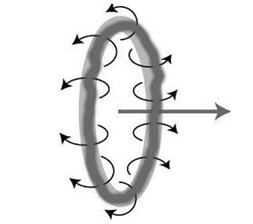
\includegraphics[width=0.4\textwidth]{graphics/theory/vortex-ring}
	\caption{Depiction of quantized vortex ring motion and induced velocity field. Source: Huang, Kerson, \textit{Quantum vorticity in nature}, arXiv.}
	\label{vortex-ring}
\end{figure}

More explicitly, it was shown \cite{donnelly_book} that in case of weak counterflow velocity $\vec{v}_{\text{ns}}$, the lifetime of vortex ring can be expressed as a simple relation:

\begin{equation}
\tau_{\text{ring}} = \frac{R_0}{2 \alpha \vert \vec{v}_{\text{ring}}(R_0)\vert}\,,
\label{ring-lifetime}
\end{equation}

where $R_0$ is the initial radius of created vortex ring.

By integrating the ring's motion equation from $R_0$ to $R(\tau) \approx a_0$ we obtain the distance travelled by the ring's center:

\begin{equation}
D_{\text{ring}} = \frac{\alpha}{1 - \alpha^{\prime}} (R_0 - a_0)
\label{ring-distance}
\end{equation}

Relations (\ref{ring-lifetime}) and (\ref{ring-distance}) are taken as a baseline in \textbf{Simulation} chapter.
\newpage

%%%%%%%%%%%%%%%%%%%%%%%%%%%%%%%%%%%%%%%%%%%%%%%%%%%%%%%%%%%%%%%%%%%%%%%%%%%%%%%%%%%%%%%%%%%%%%%%%%%%%%%%%%%%%%%%%%%%%%%%%%%%%%%%%%%%%%%%%%%%%%%%%%%%%%%%%%%%%%%%%%%%%%%%%%%%%%%%%%%%%%%%%%%%%%%%%%%%%%%%%%%%%%%%%%%%%%%%%%%%%%%%%%%%%%%%%%

{\Huge \bfseries Macroscopic view}
\addcontentsline{toc}{chapter}{Macroscopic model}
\vspace{0.3cm}

Besides NLSE and Vortex filament model, there is also a third, \textit{macroscopic} model in which the individual vortex lines are \textit{invisible} and the superfuid component of Helium-II is considered as a continuous flow of vortices. Many phenomena are similar to those in classical hydrodynamics (\textbf{Figure \ref{laminar-turbulent}}), but there emerge also new and very special type of events that can happen within superfluid Helium-II.

\begin{figure}[h]
	\centering
	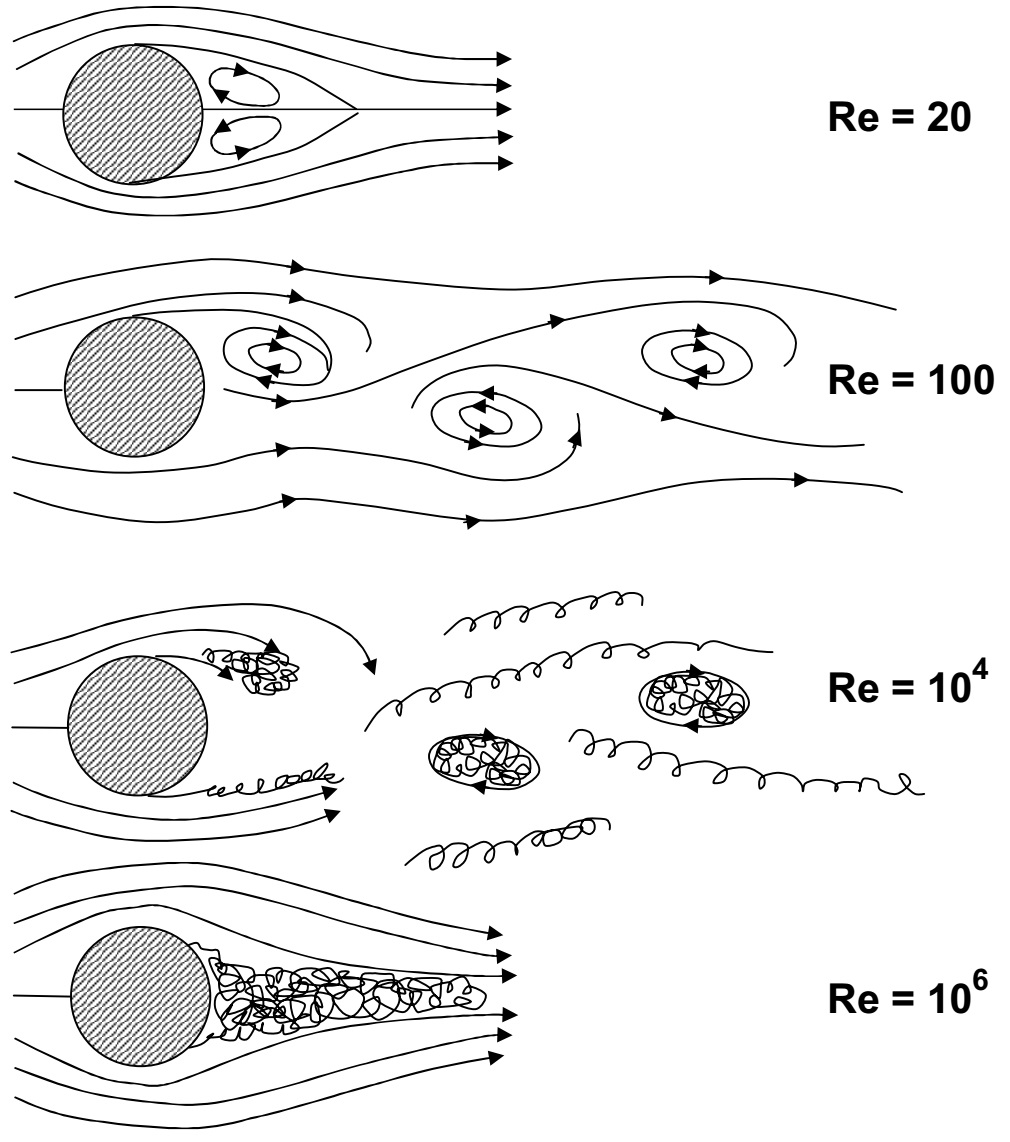
\includegraphics[width=0.5\textwidth]{graphics/theory/laminar-turbulent}
	\caption{Depiction of a classical steady flow for various Reynolds number values. Many phenomena of laminar, semi-turbulent and turbulent flows are visible in depcitions. Source: \cite{laminar-turbulence}}
	\label{laminar-turbulent}
\end{figure}

%%%%%%%%%%%%%%%%%%%%%%%%%%%%%%%%%%%%%%%%%%%%%%%%%%%%%%%%%%%%%%%%%%%%%%%%%%%%%%%%%%%%%%%%%%%%%%%%%%%%%%%%%%%%%%%%%%%%%%%%%%%%%%%%%%%%%%%%%%%%%%%%%%%%%%%%%%%%

\section{Hydrodynamics of superfluid}

Such macroscopic model is called the Hall-Vinen-Bekarevich-Khalatnikov (HVBK) model and provides a generalization of Landau's two-fluid model equations, including the presence of vortices. The superfluid is treated as a continuum and we can define a macroscopic superfluid vorticity $\vec{\Omega}_s$, despite the fact that, microscopically, the superfluid velocity field obeys $\nabla \times \vec{v}_s = \vec{0}$. The downside of this model is its assumption of spatially (not randomly) organized vortices. The common example is a rotating cylinder \cite{osborne}.\\

\newpage

The incompressible HVBK equations for normal component $\vec{v}_n (\vec{r}, t)$ and superfluid component $\vec{v}_s (\vec{r}, t)$, respectively, are \cite{barenghi}:

\begin{align}
\frac{\partial\vec{v}_n}{\partial t} + (\vec{v}_n\cdot \nabla)\vec{v}_n =& -\frac{1}{\rho} \nabla P - \frac{\rho_s}{\rho_n} S \nabla T + \frac{\eta}{\rho_n} \nabla^2 \vec{v}_n + \vec{F}_{ns}\,,
\label{motion_normal}\\
\frac{\partial\vec{v}_s}{\partial t} + (\vec{v}_s\cdot \nabla)\vec{v}_s =& -\frac{1}{\rho} \nabla P + S \nabla T + \vec{T} - \frac{\rho_n}{\rho} \vec{F}_{ns}\,,
\hspace{15mm}
\label{motion_super}
\end{align}

where we have defined:

\begin{equation}
\vec{F_{ns}} = \frac{B(T)}{2} \vec{\hat{\Omega}} \times [\vec{\hat{\Omega}}_s \times (\vec{v}_n - \vec{v}_s - \nu_s\nabla \times \vec{\hat{\Omega}})]
+ \frac{B^{\prime}(T)}{2} \vec{\Omega}_s \times (\vec{v}_n - \vec{v}_s - \nu_s\nabla \times \vec{\hat{\Omega}}_s)\,,
\end{equation}
\begin{equation}
\vec{\Omega}_s = \nabla \times \vec{v}_s\,,
\end{equation}
\begin{equation}
\vec{\hat{\Omega}}_s = \vec{\Omega}_s / \vert \vec{\Omega}_s \vert\,,
\end{equation}
\begin{equation}
\vec{T} = - \frac{\varkappa}{4\pi} \log(b_0 / a_0) \, \vec{\Omega}_s \times (\nabla \times \vec{\hat{\Omega}}_s)
\end{equation}

Here we can identify the quantities as $\vec{F_{ns}}$ (mutual friction force), $\vec{T}$ (vortex tension) and $\eta$ (viscosity parameter). Usually, $b_0$ is the intervortex spacing and can be estimated as $b_0 = (2\Omega_s \varkappa)^{-1/2}$. %Note that two-fluid equations (\ref{motion_normal}), (\ref{motion_super}) by Landau can be achieved by neglecting $\vec{F}$ and $\vec{T}$.
The HVBK equations have well-defined limiting cases:

\begin{itemize}
	\item $T \rightarrow T_{\lambda}$: In this case $\rho_s \rightarrow 0$ and the normal fluid motion equation (\ref{motion_normal}) becomes the classical Navier-Stokes equation with viscosity term.

	\item $T \rightarrow 0$: In this case $\rho_n \rightarrow 0$ and the superfluid motion equation (\ref{motion_super}) describes a pure (potential) superflow. Additionally, taking the classical limit ($\hbar \rightarrow 0$) would give us the pure Euler equation of inviscid fluid.
\end{itemize}

The HVBK model has been widely used with success to study the transition to classical or quantum turbulence, for estimations of critical Reynolds numbers and its temperature dependence.

\newpage

%%%%%%%%%%%%%%%%%%%%%%%%%%%%%%%%%%%%%%%%%%%%%%%%%%%%%%%%%%%%%%%%%%%%%%%%%%%%%%%%%%%%%%%%%%%%%%%%%%%%%%%%%%%%%%%%%%%%%%%%%%%%%%%%%%%%%%%%%%%%%%%%%%%%%%%%%%%%

\section{Dynamical similarity principle}

An important role in the behaviour of fluids is taken by the \textit{fluid dimensional numbers}, which are used for scalling of motion equations in fluid mechanics.

The principle of \textit{dynamical similarity} states that two flows of similar geometry have the same dynamical behaviour, if they can be characterised by the same set of suitable dimensionless parameters representing transport phenomena. In order to describe Helium-II with correct equations and with the most precision, we have to choose which dimensionless parameters are useful.

\begin{itemize}
	\item \underline{Knudsen number} (Kn): This number helps determine whether statistical mechanics or the continuum mechanics formulation of fluid should be used to model the system. Kn is defined as the ratio of the molecular mean free path $\lambda$ to a representative physical length scale $D$ (container size).\\
	If the temperature of Helium-II is set above $T > 1.0 \unit{K}$, there is a still sufficient amount of normal component and the mean free path of thermal excitations is much smaller, comparing it with container scale $\lambda \ll D$. In that case, continuum mechanics could be used as a macroscopic theory for superfluid Helium-II.

	However, if temperature is below $T < 0.6 \unit{K}$, the mean free path $\lambda$ becomes comparable with length scale $D$ and the continuum model starts to break down. Here, the system is rather described as a gas of thermal excitations.

	\item \underline{Weissenberg number} (Wi): This number relates the typical frequency of perturbations, $\omega$ , of the fluid with the characteristic time, $\tau$ that describes the relaxation of the fluid towards a thermodynamic equilibrium. The Weissenberg number is then given as a multiplication of oscillation frequency $\omega$ and the relaxation time $\tau$.\\
	Since the relaxation time of Helium-II is relatively small in temperatures above $T > 1\unit{K}$, then $\text{Wi} = \omega \tau \ll 1$, so Helium-II can be considered as a Newtonian fluid.

	Once again, if temperature is below $T < 0.6 \unit{K}$, relaxation time of thermal excitations rises rapidly, meaning $\text{Wi} \sim 1$, causing the excitations propagating ballistically.

	\item \underline{Reynolds number} (Re): Let's consider the continuum and newtonian assumptions ($\text{Kn} \ll 1$ and $\text{Wi} \ll 1$), so the fluid can be described by the raw form of Navier-Stokes (N-S) equation of motion. When we take into account also the incompressibility $\nabla \dotprod \vec{v} = \vec{0}$, the N-S for classical fluid reduces itself to its most simplest form.\\
	In case of stationary flow ($\partial \vec{v} / \partial t = \vec{0}$), N-S can be rewritten into a dimensionless form. Following these steps, there arises typical values of velocity $U$ and length scale $L$, at which there is the most significant change in velocity. Re can be expressed as a ratio of inertial and dissipative forces as $\text{Re} = U L \rho / \eta$, where $\eta$ is the dynamic viscosity of the flow field.\\
	The oscillatory case is described more in the next section.

\end{itemize}

The derivation of the \textit{dynamical similarity} phenomenon can be directly seen from inspection of the underlying motion equation (\ref{motion_normal}) with geometrically similar bodies. In the classical fluid dynamics, we use dynamical similarity and scaling arguments for expressing experimental data in terms of Reynolds numbers, drag coefficients, lift, and so on.

Alternatively, the dissipative forces may be described in terms of a dimensionless \textit{drag coefficient} $C_D$, representing the relation between \textit{drag force} $\vec{F}$ and fluid velocity $\vec{U}$, and usually takes the form:

$$
C_D \!\propto\! U^\alpha, \hspace{1cm}
\text{where}
\left\{
  \begin{array}{l l}
    \alpha=-1 & \quad \text{for laminar flow $\Re \in (0-10)$}\\
    \alpha=0 & \quad \text{for turbulent flow $\Re \in (10^3-10^5)$}
  \end{array}
\right.\,,
$$

where the first case ($C_D \propto 1/U$) represents the viscous skin friction anf the second case ($C_D \approx \text{const.}$) represents the pressu drag.\\
It is very common to plot experimentally measured dependence of drag coefficient $C_D$ against the Reynolds number, for various objects (sphere, disc, cylinder) past flow:

\begin{figure}[h]
	\centering
	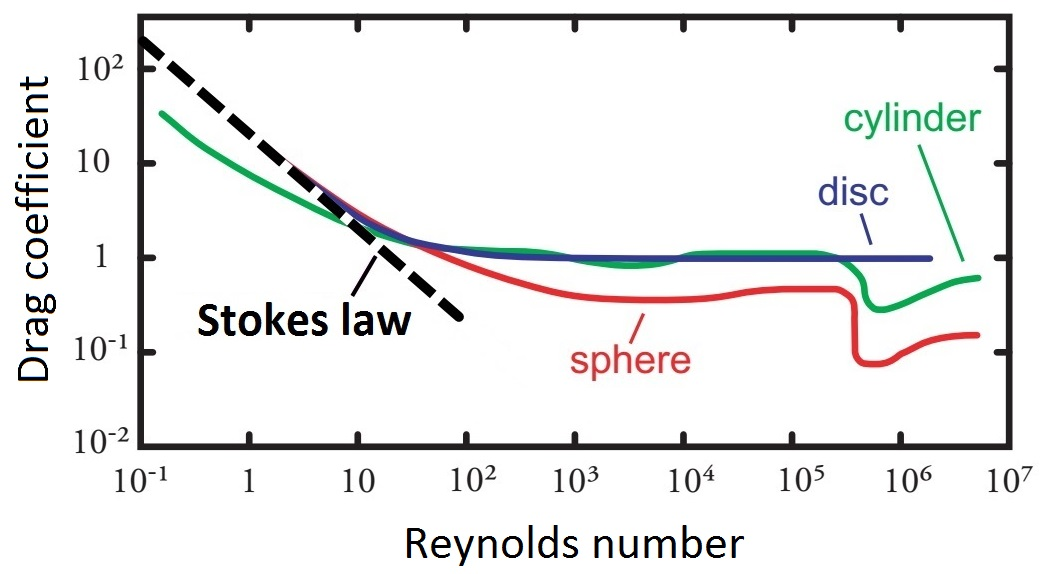
\includegraphics[width=0.7\textwidth]{graphics/theory/C-Re}
	\caption{Drag coefficients of different objects in a steady flow with changing Reynlods number. Blue line - thin disc, Green line - cylinder with drag crisis near $\Re \approx 10^6$, Red line - sphere with similar drag crisis as with cylinder, Black dashed line - laminar drag, where $C_D \propto \Re^{-1}$.}
	\label{C-Re}
\end{figure}

Dynamical similarity argument also leads to the existence of critical Reynolds number, at which the transition to turbulence in case of classical fluid occurs. Note that since superfluid Helium-II is composed of two fluids, the mentioned applies only to the normal component. The transition of superfluid component to quantum turbulence is described wider in next chapters

%%%%%%%%%%%%%%%%%%%%%%%%%%%%%%%%%%%%%%%%%%%%%%%%%%%%%%%%%%%%%%%%%%%%%%%%%%%%%%%%%%%%%%%%%%%%%%%%%%%%%%%%%%%%%%%%%%%%%%%%%%%%%%%%%%%%%%%%%%%%%%%%%%%%%%%%%%%%

\section{Oscillatory flows}

If a given body is oscillating in a classical viscous fluid, described by ordinary Navier-Stokes equation, there appears another characteristic lenght scale, identified by \cite{landau} as the \textit{viscous penetration depth}:

\begin{equation}
\delta(\omega) = \sqrt{\frac{2\eta}{\rho\omega}}\,,
\label{penetration}
\end{equation}

where $\omega$ is the angular frequency of oscilations.\\
To recognize correct characteristic length scale (whether it should be oscillating body dimension $D$ or penetration depth $\delta$), we calculate the ratio of time-dependent term $\partial \vec{v} / \partial t$ from N-S equation (\ref{motion_normal}) to the viscous term $\nabla^2 \vec{v}$. Hence, we define another dimensionless quantity, the \underline{Stokes number} $\beta$.
We calculate it \cite{stokes} as $\beta = \omega \rho D^2 / (\pi \eta)$, which can be reduced using (\ref{penetration}) to $\beta = D^2 / (\pi \delta^2)$.\\
From this, we call a situation as the \textit{high-frequency regime}, when $\delta \ll D$, so the Stokes values are $\beta \gg 1$.

\subsection*{Classical hydrodynamics}

To describe fully an oscillatory flow, the governing Navier-Stokes equations may be expressed in terms of dimensionless velocity $U$, time $T$ and positions $L$. The independent time scale is given by the angular frequency of oscillations $\omega$. Candidates for characteristic lenght scale $L$ may lead to the body size $D$, surface roughness, or the viscous penetration depth $\delta(\omega)$.

In the high frequency limit (directly from \ref{penetration}) $\omega \gg 2\eta / (\rho D^2)$, depending on body geometry, one can reach $\delta(\omega) \ll D$ and say that fluid oscillates in
high Stokes regime \cite{universal_scaling} with $\beta = D^2 / (\pi \delta^2) \gg 1 $. Also, when also the surface roughness exceeds $\delta$, the N-S equation may be expressed using only one dimensionless parameter: an \textit{oscillatory Reynolds number} $\Re_{\delta} = \delta U \rho / \eta$.

\subsection*{Superfluid Helium-II}

Assuming two independent velocity fields $\vec{v}_n (\vec{r}, t)$, $\vec{v}_s (\vec{r}, t)$ in superfluid Helium-II, the above thoughts are applicable for the oscillatory viscous flow of the normal component $\vec{v}_n$. We therefore define the high frequency limit for normal component as:

\begin{equation}
\delta_n = \sqrt{\frac{2\eta}{\rho_n\omega}}\,,
\hspace{1cm}
\text{Dn} = \frac{U \delta_n \rho_n}{\eta}
\label{donnelly}\,,
\end{equation}

We will call the oscillatory Reynolds number for normal component in superfluid Helium-II as a \textit{Donnelly number} (Dn, after Russell J. Donnelly, who as first came with this (\ref{donnelly}) idea.

At low velocities, below the critical thresholds to create either classical or quantum turbulence, the flow of the superfluid component is purely potential and the normal component exhibits laminar viscous flow.

If the typical body curvature is of order $1/D$, the surface may be described as if consisting of many planar elements. In this case it is shown \cite{universal_scaling} that we can write for the average dissipated energy:

\begin{equation}
\langle \dot{E} \rangle =
\frac{1}{2} \alpha \xi U_0^2 S_{eff} \sqrt{\frac{\eta \rho_n \omega}{2}}\,,
\label{energy_loss}
\end{equation}

where $U_0$ is the velocity amplitude, $S_{eff}$ the effective surface, $\alpha$ the mutual friction constant and $\xi$ the integral of velocity profile along the resonator. The total energy of an oscillator is given as $E = \xi m U_0^2 / 2$ and moreover, we define a fluidic quality factor $Q_f$ of an oscillator for a single oscillation as:

\begin{equation}
1 / Q_f = \frac{\langle \dot{E} \rangle}{\omega E} = \frac{\alpha \rho_n S_{eff} \delta_n}{2m}
\label{quality}
\end{equation}

From (\ref{energy_loss}), one can also derive the peak dissipative force (during a period of oscillation) and the dimensionless drag coefficient related to the normal component:

\begin{equation}
F_0 = \frac{2 \omega \langle \dot{E} \rangle}{U_0}
= \alpha \xi \omega S_{eff} U_0 \sqrt{\frac{\eta \rho_n \omega}{2}}
\hspace{5mm}
\rightarrow
\hspace{5mm}
C_D^{\,n} = \frac{2 F}{A \rho_n U_0^2} = \frac{2 S_{eff}}{A U_0} \sqrt{\frac{\eta \omega}{\rho_n}}\,,
\label{drag_normal}
\end{equation}

where $A$ is the cross-section of the body perpendicular to flow. According to dynamical similarity principle, the drag coefficient (\ref{drag_normal}) can be expressed as a function of the dimensionless Donnelly number (\ref{donnelly}):

\begin{equation}
C_D^{\,n} = \Phi / \text{Dn}\,,
\end{equation}

where number $\Phi$ is determined by the oscillating body geometry. Clearly, the laminar case of normal component is fully described by the hydrodynamic laws. In turbulent case, we expect a constant value for $C_D^{\,n}$ as long, as only normal component contributes to the drag force (no quantum turbulence).

\section{Quantum turbulence}

Turbulence of superfluid component can be viewed as a tangle of vortex lines. In this case quantized vortices can be nucleated either \textit{intrinsically} (such process requires critical velocities of order $10 \unit{m/s}$) or \textit{extrinsically}, by stretching and reconnections of seed vortex loops. The initial vortices in the extrinsical case are the remnant vortices, which always exist in macroscopic samples of Helium-II . In many types of flow the critical velocity for extrinsic vortex nucleation is observed to be in order $\sim\unit{cm/s}$.

The superfluid component becomes turbulent at some critical velocity $U_C$ and therefore, we expect an increase in drag coefficient $C_D$ much above the possible dependence caused by turbulence of normal component. The process of self-reconecting remnant vortices was well studied \cite{universal_scaling} and the related critical velocity is expected to scale as $U_C \propto \sqrt{\varkappa \omega}$, where $\varkappa$ is the circulation quantum. Hence, it is convenient to define a dimensionless velocity $\hat{U}$ with related drag coefficient $C_D^{\,s}$ as:

\begin{equation}
\hat{U} = U_0 / \sqrt{\varkappa \omega}
\hspace{5mm}
\rightarrow
\hspace{5mm}
C_D^{\,s} = \frac{2 F_0}{A \rho_s U_0^2} = \frac{2 F_0}{A \rho_s \varkappa \omega \hat{U}^2}\,,
\label{drag_super}
\end{equation}

In case of turbulent superfluid component with velocities sufficiently above critical values, we expect both component to be coupled due to the mutual friction. In this case, both components contribute to the pressure drag, and drag coefficient must be calculated classicaly as $C_D = 2F / (A\rho U^2)$. where $\rho$ is the total density of Helium-II.

\newpage

\subsection*{Ultra-low temperature regime}

In classical fluids, when the mean free path $\lambda$ of particles becomes comparable to a lenght scale $D$ of the system ($\text{Kn} \sim 1$), the continuum model of the fluid starts to break down and the system cannot longer be described by the Navier-Stokes equations. Similar arguments go when the angular frequency of oscillatory flow $\omega$ becomes comparable with the relaxation time $\tau$ of the fluid towards thermodynamic equilibrium ($\text{Wi} = \omega \tau \sim 1$).\\
Here, the system is described as a gas of thermal quasiparticles propagating
ballistically through a physical vacuum. Therefore, such system state is called as \textit{ballistic regime}.

In practice with superfluid Helium-II, such situation is usually reached by cooling fluid  down to ultra-low temperatures. Below $T < 1\unit{K}$, the normal component accounts for less than $1\%$ of the total density, but required cooling to obtain ballistic regime (\textbf{Figure (\ref{ballistic})}) is below $T < 0.6\unit{K}$ (here the Helium-II is better described as a gas of thermal quasiparticles than a fluid).

\begin{figure}[h]
	\centering
	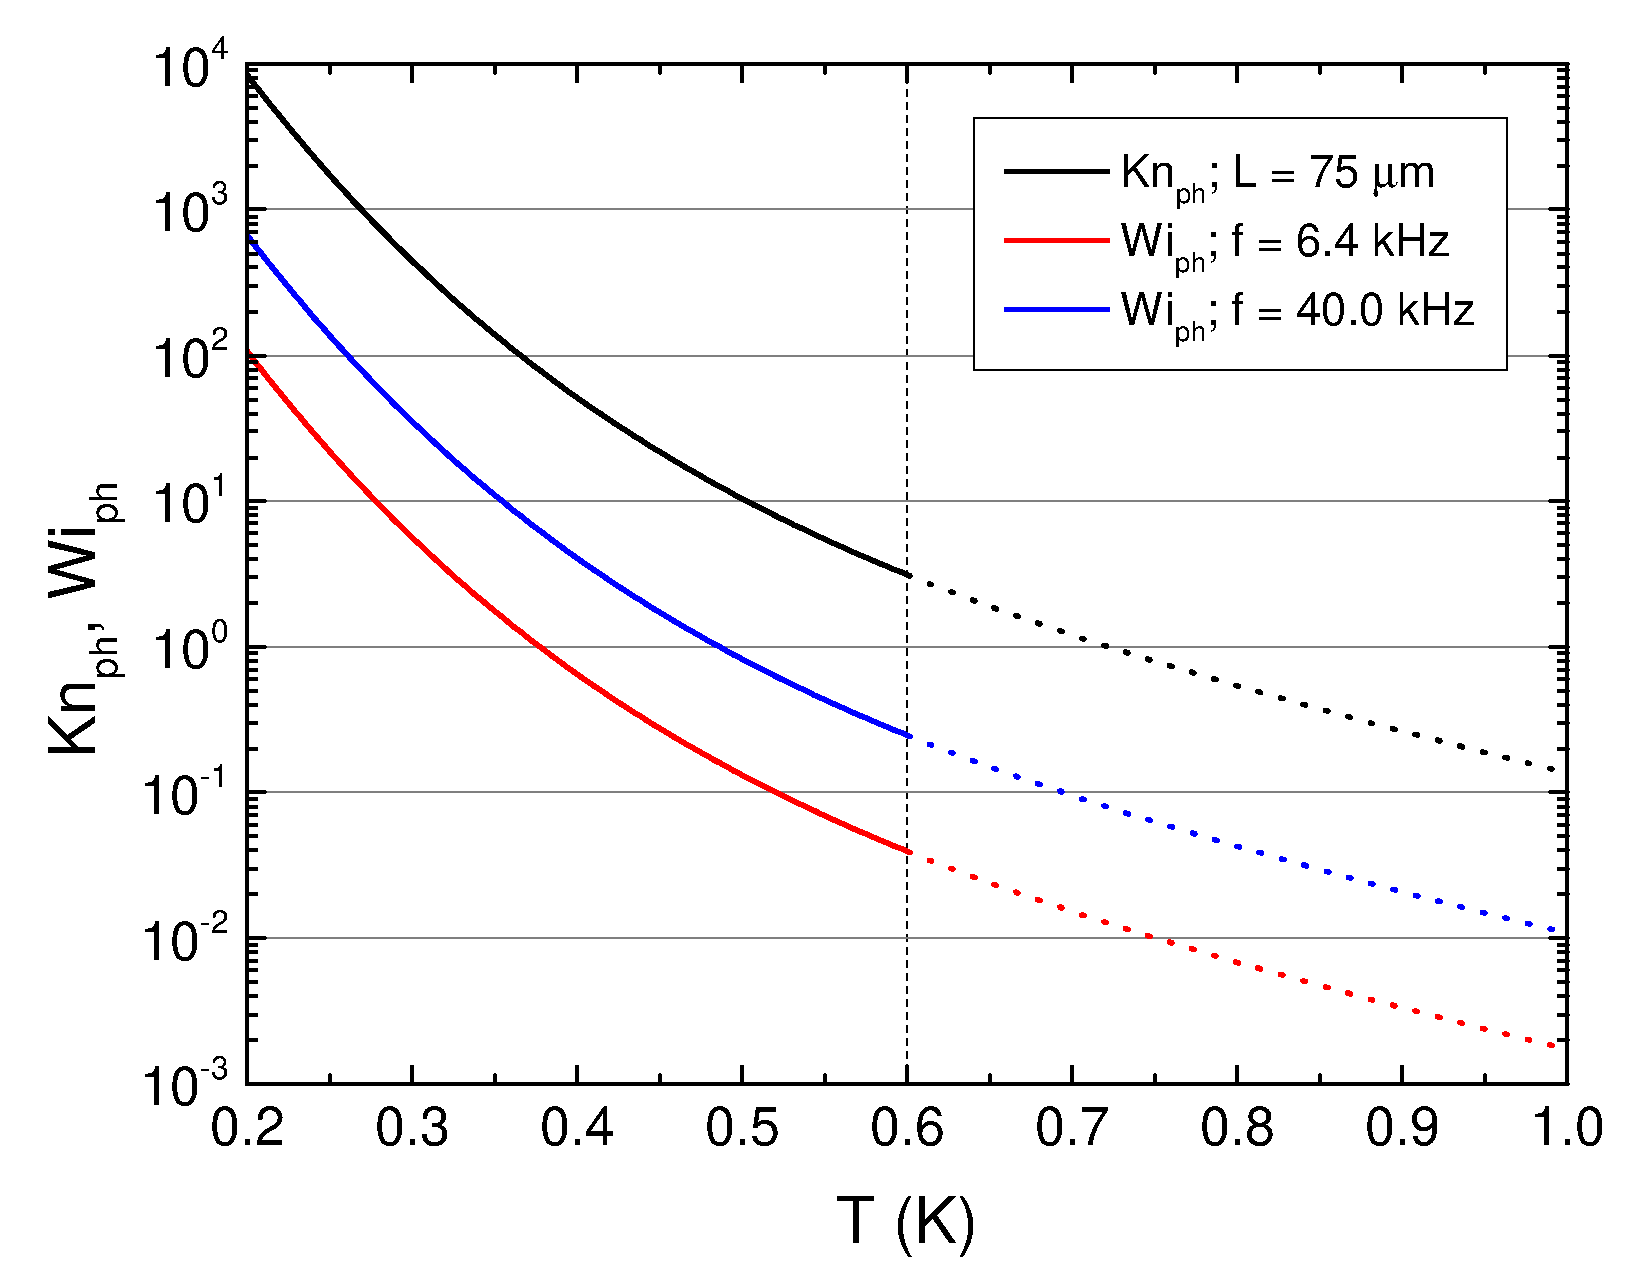
\includegraphics[width=0.7\textwidth]{graphics/theory/ballistic}
	\caption{Phonon Knudsen number and Weissenberg numbers plotted against temperature for different oscillators. The dashed line separates the interval $T < 0.6\unit{K}$, where the ballistic regime takes a place. Source: \cite{universal_scaling}}
	\label{ballistic}
\end{figure}

\newpage

\subsection*{Universal scaling}

A study was conducted in order to solve the Stokes' second problem with an oscillating plane in viscous fluid, using pure Boltzmann kinetic equation. This solution is used to derive a universality relation valid in the high frequency limit (with no turbulence present) across both Newtonian and non-Newtonian regimes of the fluid. Using scaling function $f(\omega \tau)$, the authors derived \cite{universal_scaling} the relation for the quality factor:

\begin{equation}
1 / Q_f = \frac{\alpha S_{eff}}{m} \sqrt{\frac{\eta \rho_n}{2\omega}} f(\text{Wi})
\end{equation}

In \textbf{Results} we use this form of universality scaling for comparison against experimental data collected in temperature ranges $T < 0.6\unit{K}$ or $T > 1\unit{K}$.

\subsection*{Multiple critical velocites}

Here is briefly commented the transition to quantum turbulence regime observed at very low temperatures ($T \ll 1\unit{K}$). A couple of experimental studies in milliKelvin temperatures reported \cite{crit-velocity} the existence of more critical velocities related with superfluid component flow within single experiment:

\begin{itemize}
	\item \underline{First critical velocity} is related to the formation of pinned vortex loops at the surface of oscillating body - possibly forming a thin layer with different hydrodynamic behaviour which increases the effective mass of the oscillating object. Such critical velocity is hard to observe at higher than ultra-low temperatures.

	\item \underline{Second critical velocity} is a consequence of vortex rings escaping from the oscillator body into the superfluid bulk and eventually forming a vortex tangle. Here the sudden raise of drag is observed, usually with hysteresis effect.

	\item \underline{Third critical velocity} is the highest critical velocity which can be observed. The origin of this velocity is linked to the development of larger quantized vortex structures, which in larger scale start to mimic the classical turbulence. Such velocity is in order $\approx \unit{m/s}$ and moreover, very likely screened by the influence of the normal component turbulence. Therefore, not likely reachable within experiments reported in this Rhesis.
\end{itemize}

% When both velocities of Helium-II are high enough, we expect the turbulent regime on both sides to be coupled due to mutual friction and contributing to the drag. In such situation, we are forced to use classical hydrodynamic metrics: drag coefficient $C_D = 2F / (A\rho U^2)$ and Donnelly number $D = U \delta / \nu$. Recent researches also hint that both classical turbulent and quantum turbulent regimes can exist separately with low interaction.
%
% Note that all presented approches are only approximate, since they are neglecting flows near the oscillating body, evaporation processes, sound emissions and other corner-case effects.

% \section{Second sound}
%
% Ordinary sound (the wave of density $\rho$ and pressure $P$) in Helium-II is called \textit{first sound}. In such process, temperature $T$ and entropy $S$ is conserved and $\vec{v}_n$ and $\vec{v}_s$ oscillate in phase with each other ($\vec{v}_n(t) \approx \vec{v}_s(t)$). On the contrary, by combination of two-fluid motion and continuity equations, one obtains the wave equation also for the temperature $T$ and entropy $S$. In such case the velocities obey an antiphase oscillation ($\rho_n(t) \vec{v}_n(t) \approx - \rho_s(t) \vec{v}_s(t)$) and remains $\rho$ and $P$ constant.
%
% \begin{figure}[h]
% 	\centering
% 	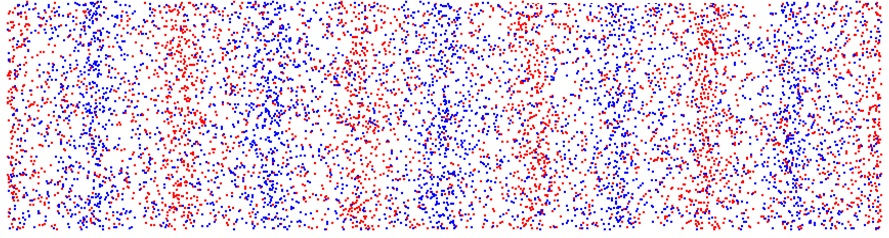
\includegraphics[width=0.99\textwidth]{graphics/theory/ss_1}
% 	\caption{here will come more proper picture}
% 	\label{ss_1}
% \end{figure}
%
% \begin{figure}[h]
% 	\centering
% 	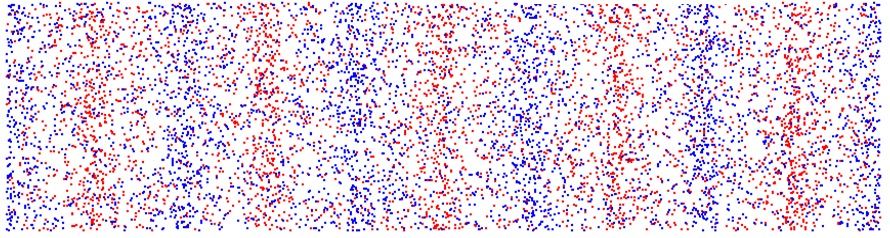
\includegraphics[width=0.99\textwidth]{graphics/theory/ss_2}
% 	\caption{here will come more proper picture}
% 	\label{ss_2}
% \end{figure}
%
% In early Vinen's observations, the exponentially damped velocity of second sound wave, propagating through two-fluid medium, was derived from motion equations:
%
% \begin{equation}
% \vec{v}_{\ind{ns}} \propto e^{-\alpha \vert \vec{r} \vert} \vec{\hat{e}}_{\vec{r}}(\vec{k},\vec{r},\omega,t)\,,
% \end{equation}
%
% where $\alpha$ is the attenuation coefficient. When considering homogeneous chaotic distribution of vortex tangle, one can also derive the formula for the attenuation factor:
%
% \begin{equation}
% \alpha = \frac{B\kappa L}{6 \vert \vec{c}_2\vert}
% \label{alpha_mean}\,,
% \end{equation}
%
% where $B$ is the first mutual friction parameter and $\vec{c_2}$ is the initial second sound velocity. This velocity was experimentally examined and there was found a plateau near the value $20 \unit{m/s}$, which is desirable during experiments (stability against small temperature changes):
%
% \begin{figure}[h]
% 	\centering
% 	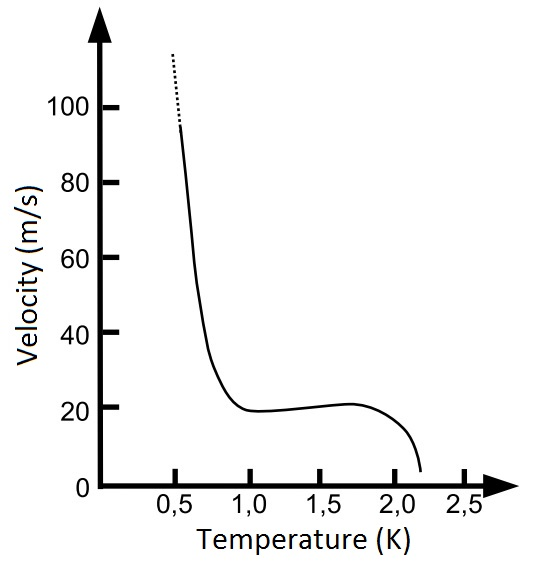
\includegraphics[width=0.4\textwidth]{graphics/theory/ss_velocity}
% 	\caption{velocity of the second sound with temperature}
% 	\label{ss_velocity}
% \end{figure}
%
% In this work, the phenomenon of second sound attenuation is used for detection of quantized vortices, which naturally appear within Helium-II. There is written much more about the method itself within the Experimental Approach part.

\newpage

%\chapter{Experimental Approach}

Experiments presented and analysed in this Thesis were conducted in Prague, with members of department of low-temperature physics, under Charles University.

Many experimental methods are known and were conducted in order to launch the quantum turbulence: by an oscillating objects (wires, tuning forks, oscillating discs, etc.) or by \textit{coflow} and \textit{counterflow} techniques (in other words, using indirect flow sources).

In our investigation, we used entirely 3 types of oscillating objects: vibrating NbTi wire, oscillating disc and tuning fork oscillator, driven by alternating source Agilent A33220 and measured by SR830 amplifying lock-in, using an I/V converter with an conversion ratio 1000 V/A \cite{skyba}. We measured both the in-phase and anti-phase componentes and also the quadratures of signals.

Experimental data of vibrating wire and oscillating disc are included and analysed in this Thesis, but a pure experimental work by the author of this Thesis, was performed only with the tuning forks.

In this chapter, we introduce the technical details of all used oscillators, their integration within the whole experimental setup and in the end, the measurement techniques performed on these oscillators.

\newpage

\section{Apparatus}

All measurements were performed in a helium cryostat, cooled down to the desired temperatures using a rotary and Roots pump, and stabilized (with errors of a few mK) either manually or using a Lake Shore temperature controller Model 340. The most of used technologies are captured in a photograph in \textbf{Figure \ref{cryostat}}.

\begin{figure}[h]
	\centering
	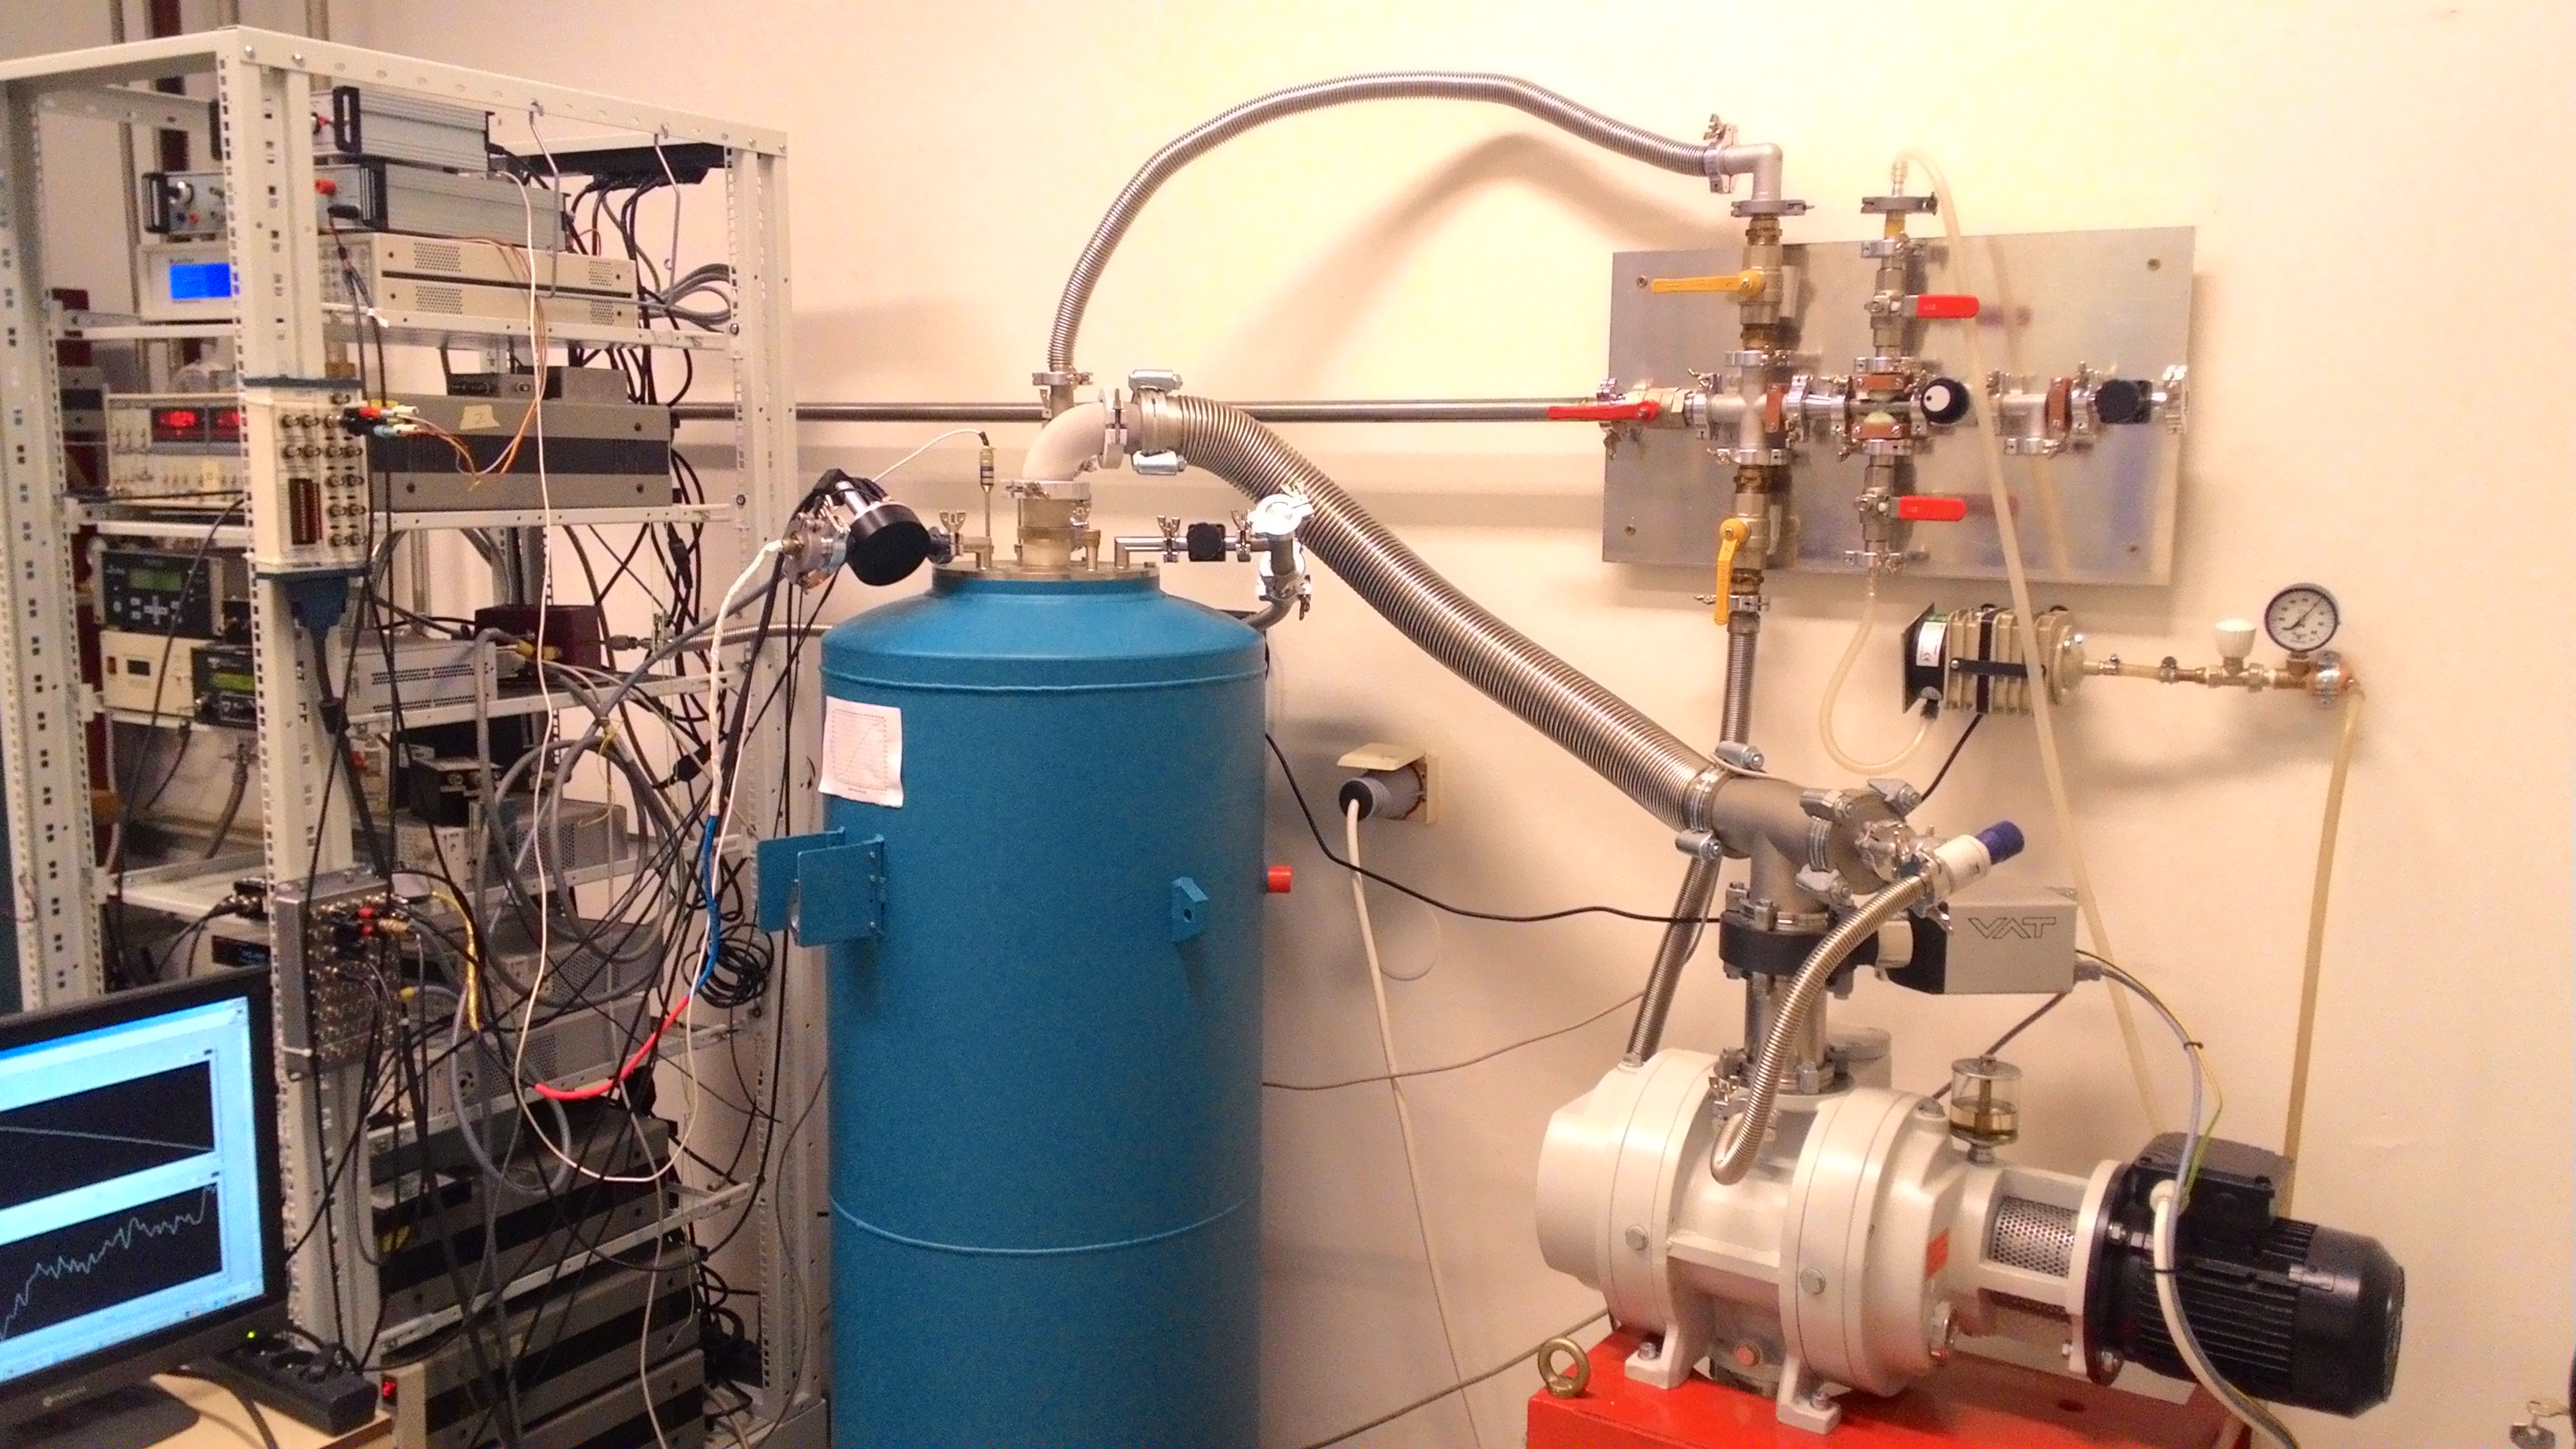
\includegraphics[width=0.9\textwidth]{graphics/exp/apparatus}
	\caption{A photograph of the experimental setup. \underline{From left}: source generators Agilent A33220, amplifying lock-ins SR830 with an I/V converters, cryostat, gas handling system (pipes) for emerging gas, rotary and Roots pump. Source: \cite{bakalaris}}
	\label{cryostat}
\end{figure}

Our chosen studied temperatures are from a wide range from a little below the transition temperature $\sim 2.17\unit{K} \gtrsim T_{\lambda}$ to the lowest (experimentally) possible one $ \sim 1.35\unit{K}$. We also performed series of measuremens in the area far above the transition temperature $\sim 3 \unit{K} > T_{\lambda}$ in order to test all used components.\\
The studied range $(1.35\unit{K} - 2.17\unit{K})$ allows access to the wide range of normal/superfluid components ratios of the two-fluid model ($\rho_s / \rho_n \ll 1$ at $T\lesssim 2.17\unit{K}$ and $\rho_s / \rho_n \approx 16$ at $T\sim 1.35\unit{K}$).

Measurements at ultra-low temperatures $T < 0.6\unit{K}$ in the ballistic regime of Helium-II were performed on a Leiden Cryogenics MNK126-400 dilution refrigerator with a base temperature below $10 \unit{mK}$. The description of sub-Kelvin measurements is not included in this chapter, but is discussed in sufficient detail in \cite{universal_scaling}. However, refrigerator results are analysed in the last section of \textbf{Results} chapter in order to test the validity of the \textit{uniform scaling} concept, introduced in the last secton of the \textbf{Theoretical Background}.

\newpage

The tuning fork oscillators were tightly attached in the inner space of the cylindrical \textit{second-sound resonator} cavity, also capable to produce the second sound on the one side and receive it on the other side. We drilled a small hole to the resonator body in order to fill it with Helium-II.

This resonator (\textbf{Figure \ref{resonator}}) was  was attached at the bottom  of the \textit{insert} - a large metallic construction holding all measuring micro-devices, thermometers and coaxial cables.

\begin{figure}[h]
	\centering
	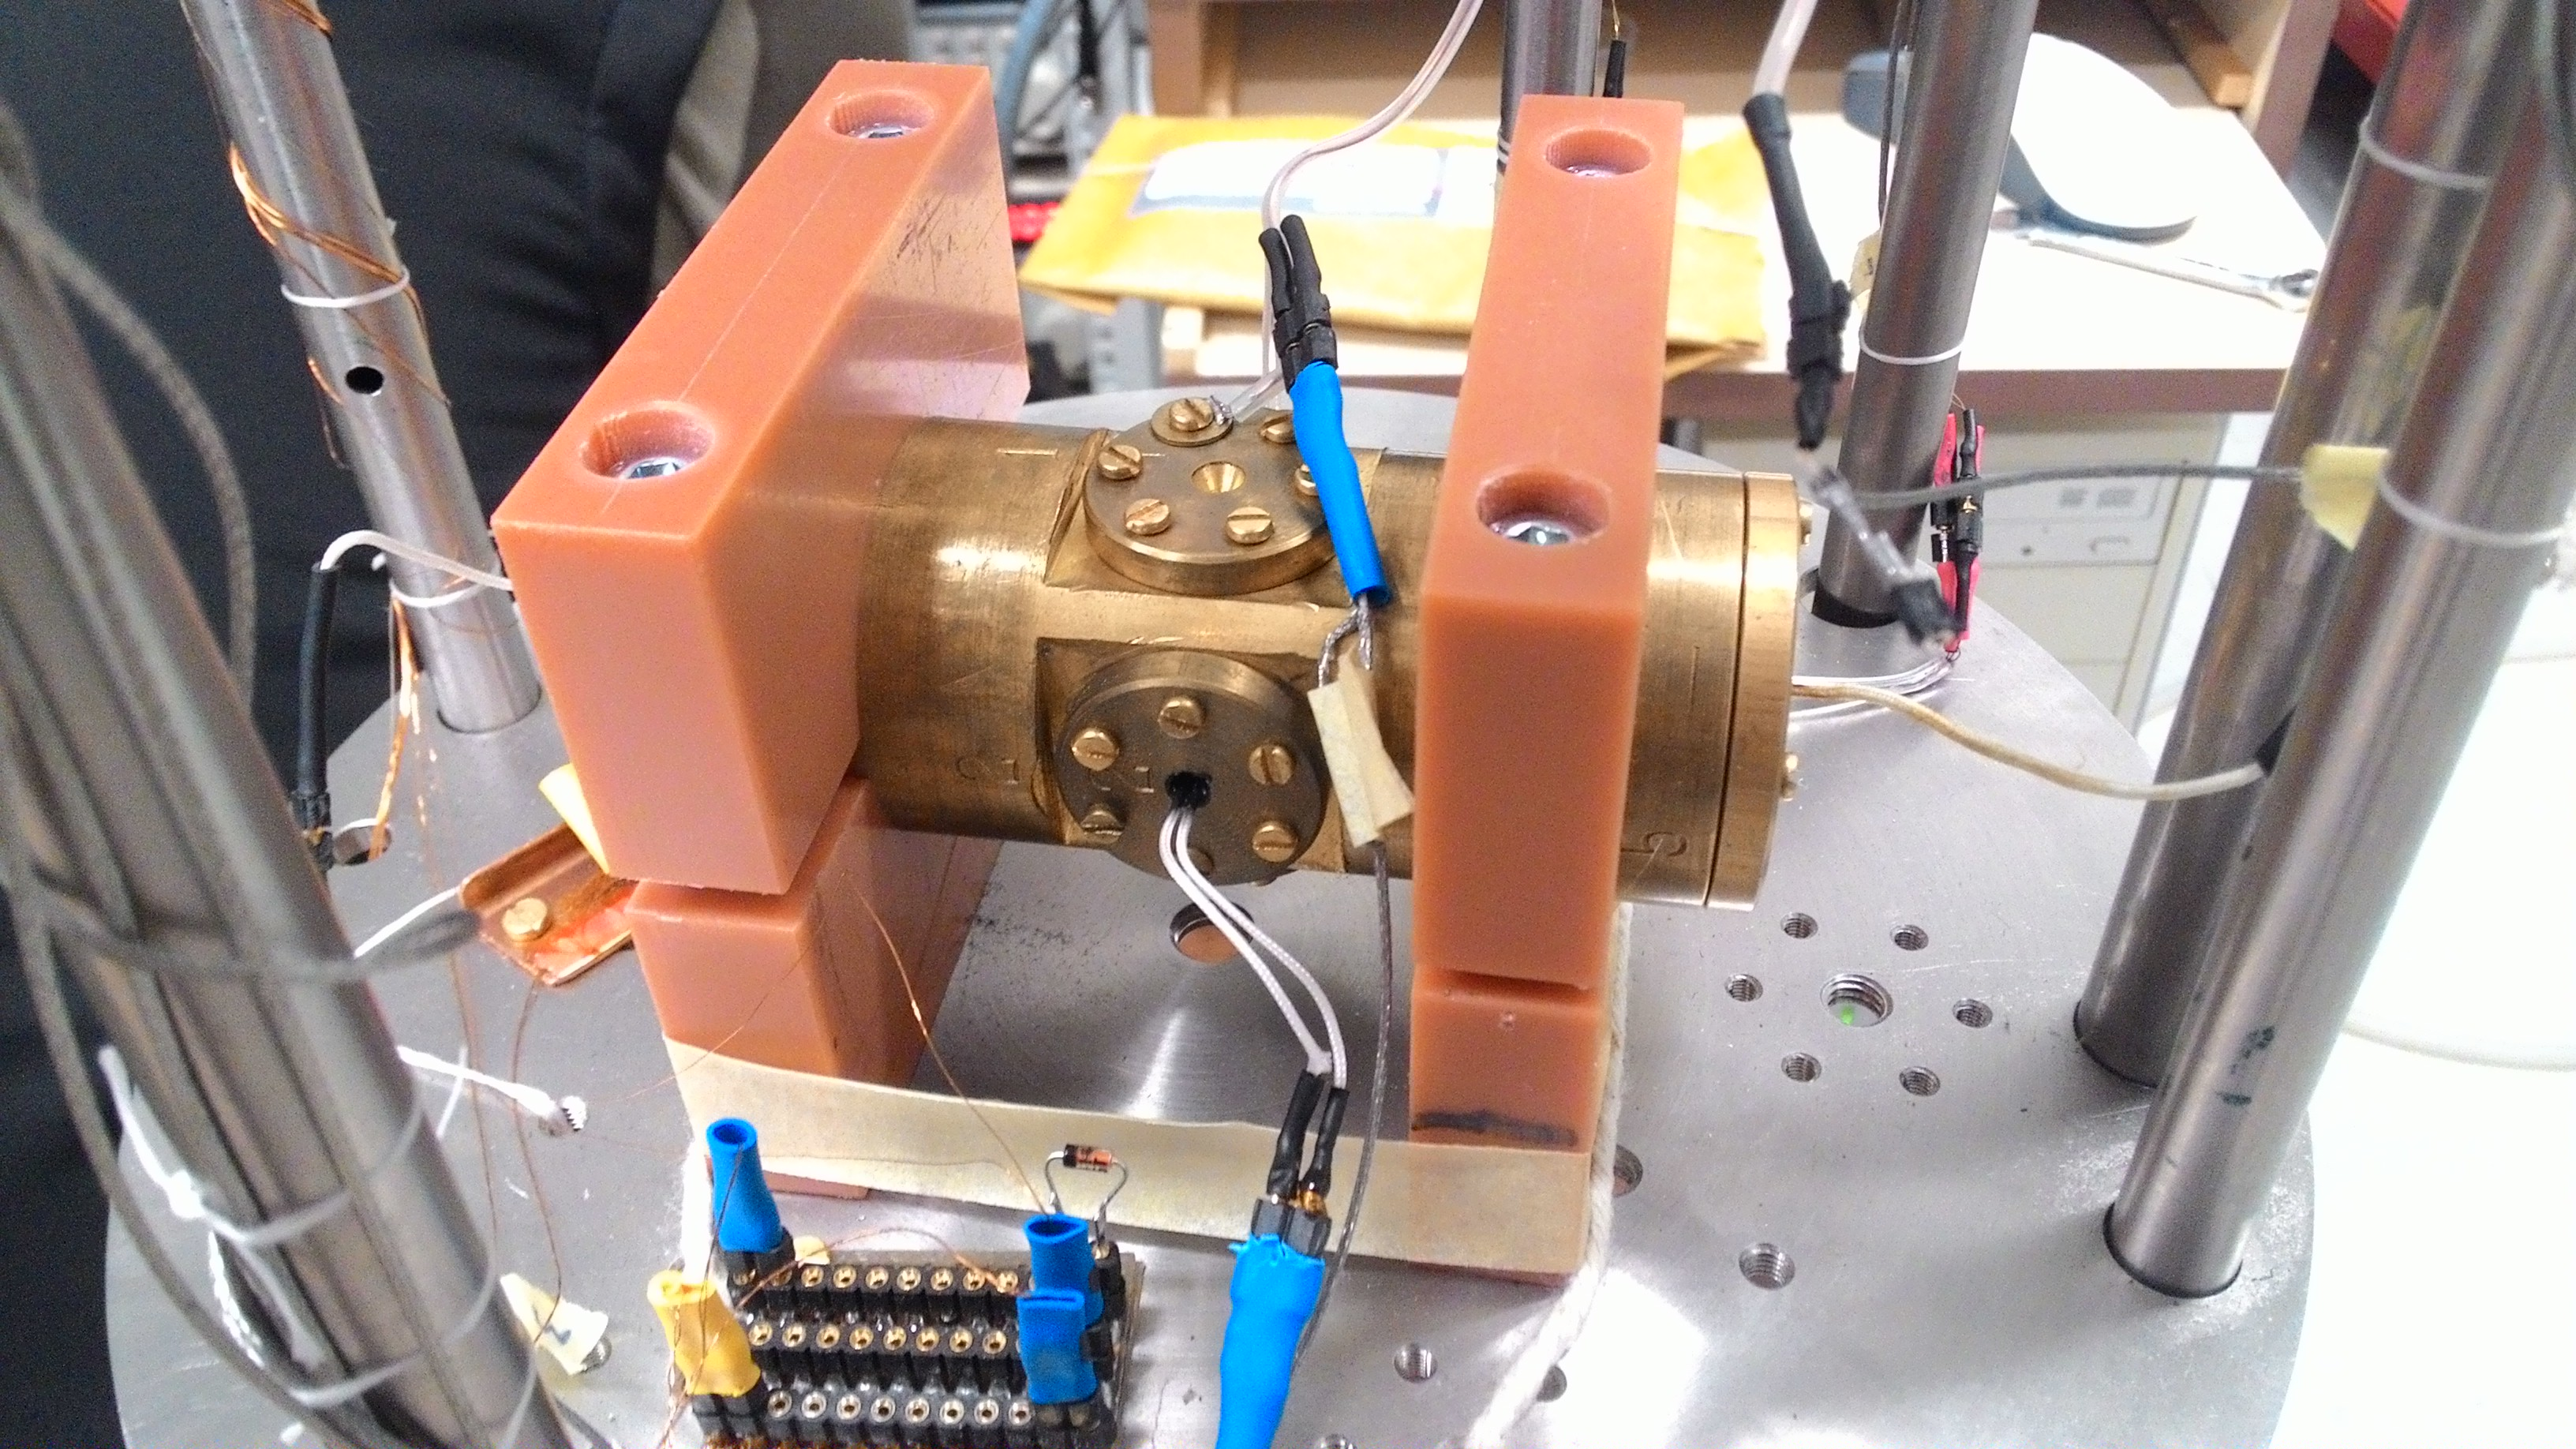
\includegraphics[width=0.9\textwidth]{graphics/exp/chamber}
	\caption{A photograph of the second-sound resonator attached at the bottom of metallic insert with cables and thermometers. Source: \cite{bakalaris}}
	\label{resonator}
\end{figure}

To obtain the best results at low temperatures, the cryostat containing oscillators was repeatedly flushed with pure liquid $\He$ from Dewar transport container. After this pre-cooling step, the liquid $\He$ was transferred using a siphon.

The inner space of resonator was additionally separated from the outer part (cryostat body) by a sinterred copper, forming a solid mass of material by pressure. This ensures that no parasitic helium ices microparticles or other inpurities will interfere with the oscillators inside of resonator.


\newpage

\section{Resonators}

In this section we briefly describe the principles of micro-scale oscillators used in experiments with Helium-II.

\subsection{Vibrating Wire}

Vibrating NbTi wire resonator consists of a semi-circular loop of wire inserted to a vertical magnetic field $\vec{B}$, as shown in \textbf{Figure \ref{wire}}. As we turn on the alternating current flux $\vec{j} \propto e^{i\omega t}$ inside the wire, these currents forces the wire to oscillate due to Lorentz force $\vec{F}_L \propto \vec{j} \times \vec{B} $. As the wire moves through the field, the Faraday voltage is induced of magnitude \cite{wire}:

\begin{equation}
V = - \frac{\text{d} (\vec{B} \dotprod \vec{S})}{\text{d} t}
\sim \frac{\pi}{4} BDU\,,
\end{equation}

where $\vec{S}$ is the area vector, enclosed by the wire loop and $D$ is the distance between wire's legs. Experimentally used magnetic field was about $\approx 170 \unit{mT}$ with an uncertainty of $\pm 10 \unit{mT}$.

\begin{figure}[h]
	\centering
	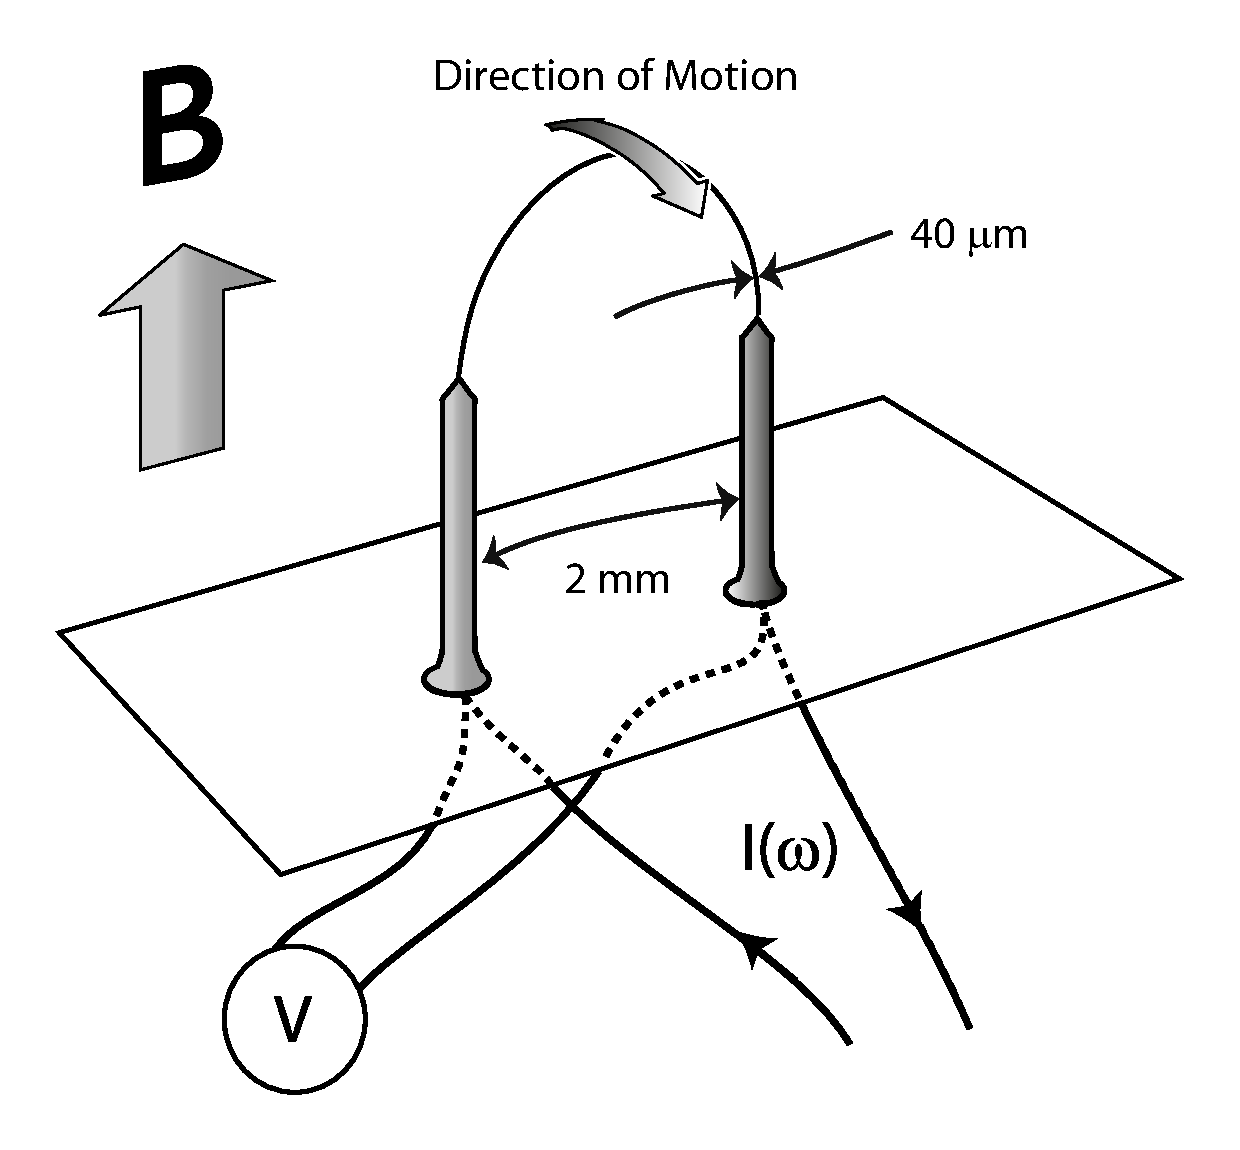
\includegraphics[width=0.5\textwidth]{graphics/exp/wire}
	\caption{Schematic diagram of the vibrating wire resonator. Source: \cite{universal_scaling}}
	\label{wire}
\end{figure}

\newpage

\subsection{Oscillating Disc}

The torsional oscillator consists of a $50 \mu\text{m}$ wire  with a glass disc fixed to
the wire at its midpoint. The disc is $1\unit{mm}$ thick with a diameter of $40\unit{mm}$. A schematics is sketched in \textbf{Figure \ref{disc}}.\\
Sixteen black marks around the circumference of the disc are used to determine the deflection and angular velocity of the disc from recorded video sequences.

\begin{figure}[h]
	\centering
	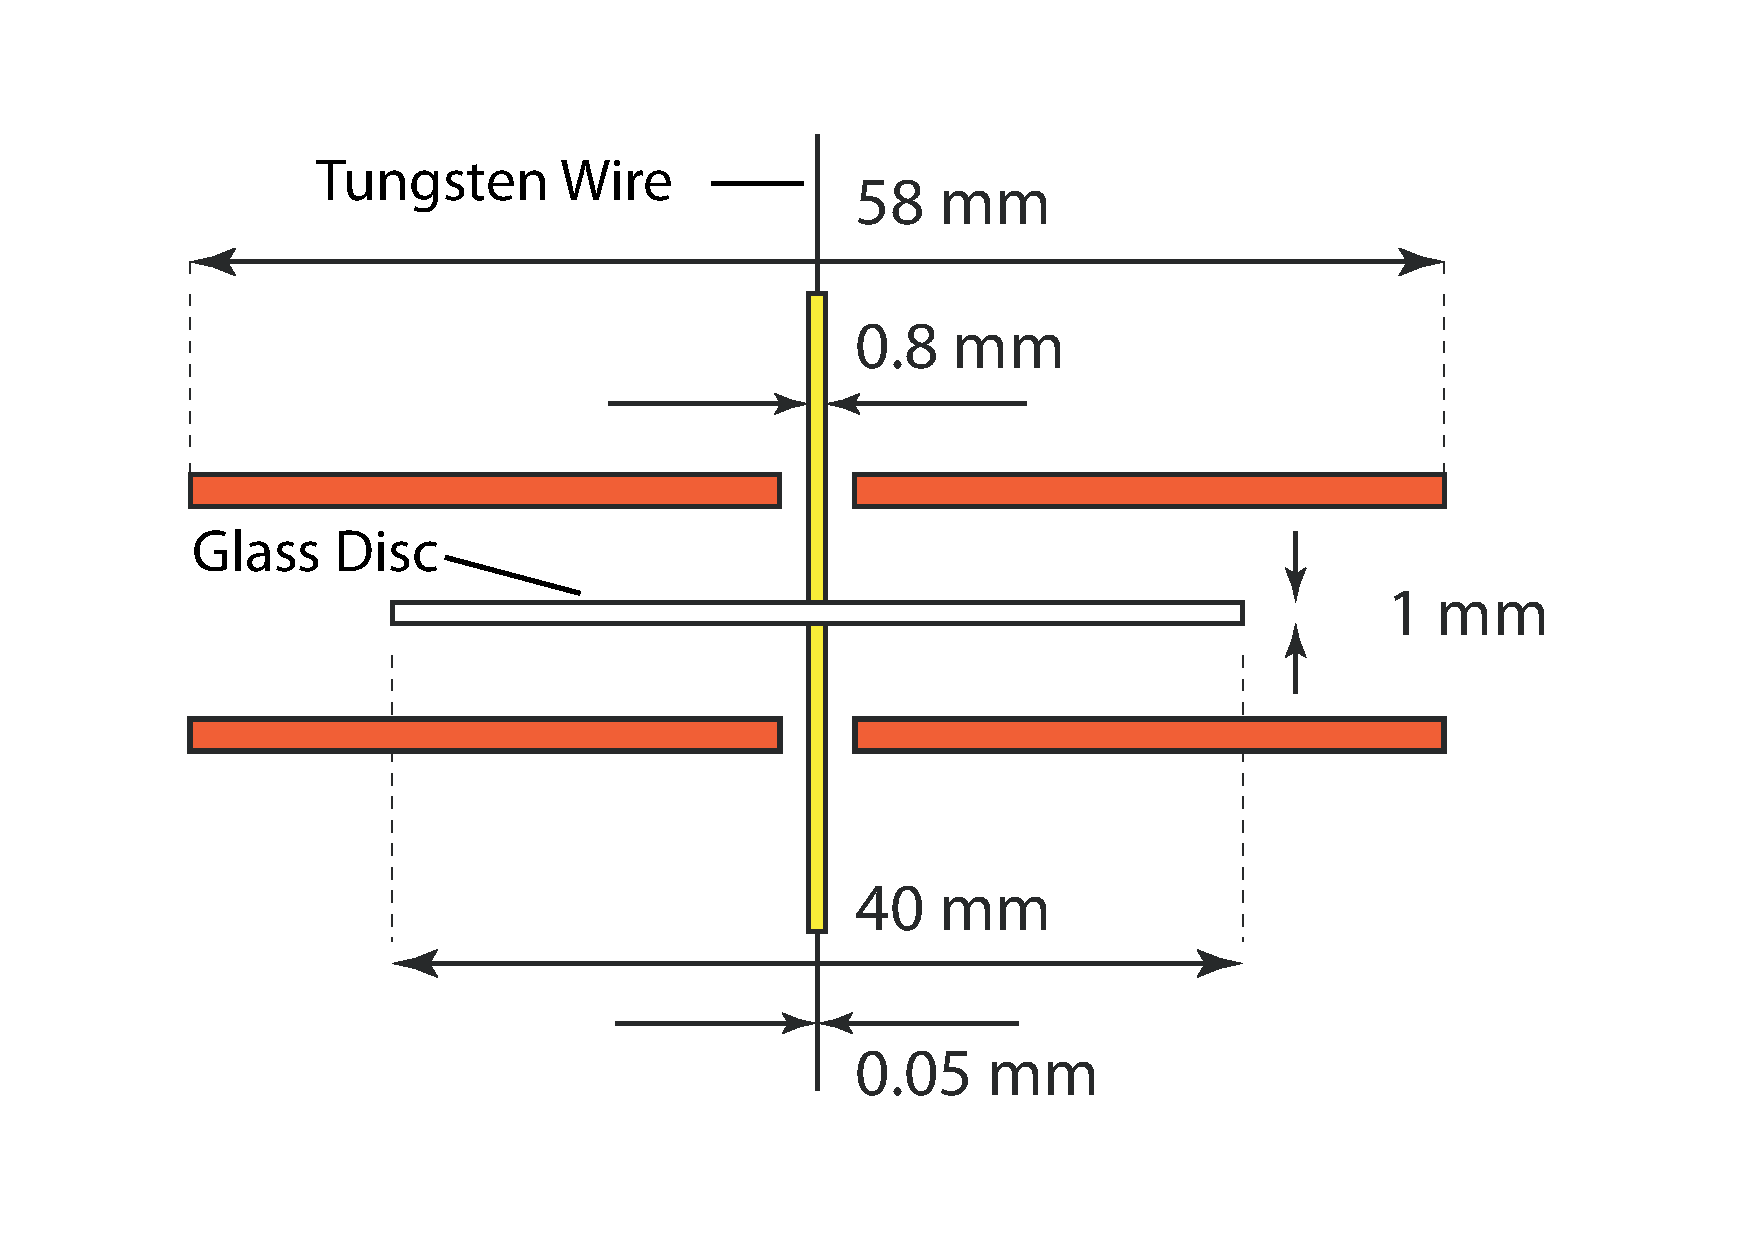
\includegraphics[width=0.7\textwidth]{graphics/exp/disc}
	\caption{Schematic diagram of the torsionally oscilating disc. Source: \cite{universal_scaling}}
	\label{disc}
\end{figure}

The raw data is in the form of video recordings of the disc motion and fairly complex post-processing method was required to extract quantities. The optical distortion from the lenses and the curved walls of the cryostat are negligible. More details about data processing can be found in \cite{universal_scaling}.

\subsection{Tuning Fork}

Quartz tuning forks (TF) are commercial piezoelectric oscillators with a well-calibrated resonant frequency. They are usually used as frequency standards in watches or as force sensors in microscopes. Also, TFs have started to be widely used in cryogenic Helium II experiments \cite{forks}.

In our experimental setup, we used the fork of following dimensions: prongs length $ \mathcal{L} = 3.50\unit{mm} $, prongs width (perpendicular to the fork plane) $ \mathcal{W}=75 \mu\unit{m} $, thickness $ \mathcal{T}=90\mu\text{m} $ prongs interdistance $ \mathcal{D}=90\mu\text{m} $.
The same type of fork was also used and discussed in \cite{fork-exp} \cite{multiple-vels} A sketch of the fork architecture is depicted in \textbf{Figure \ref{fork}}:

\begin{figure}[h]
	\centering
	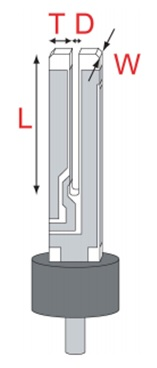
\includegraphics[width=0.2\textwidth]{graphics/exp/quartz}
	\caption{Schematic diagram of the quartz tuning fork. Source: \cite{bakalaris}}
	\label{fork}
\end{figure}

There are several achievable resonant modes at which the fork can oscillate. We chose to work with the \textit{fundamental} one at $f_0 \sim 6400 \unit{Hz}$ and with the first \textit{overtone} one at $f_1 \sim 40\,200 \unit{Hz}$.\\
The fork is driven by applying an alternating voltage $V(t) \propto e^{i\omega t}$ from a generator to the metalic plates (deposited on fork surface). The piezoelectric effect causes a tension resulting in a force, which is proportional to the applied voltage. In fundamental mode, the fork exhibits an anti-phase oscillating motion of its prongs with a single node. In case of overtone, there would be just two nodes. The fork's flexion induces a piezoelectric current $I(t)$ which is proportional to the velocity $U(t)$.

The conversion relations between applied $V(t)$, measured $I(t)$ and mechanical properties $F(t)$, $U(t)$ are given \cite{forks} as:

\begin{equation}
F(t) = \frac{1}{2} a_{f} V(t)\,,
\hspace{1cm}
U(t) = \frac{I(t)}{a_{f}}\,,
\label{fork_conversions}
\end{equation}

where $a_{f}$ is the so-called \textit{fork constant}. This constant can be derived from a fork's geometry, material properties and its oscillation mode. The formula the fork constant calculation is given usually by a deflection measurement:

\begin{equation}
a_{f} = \sqrt{4\pi m_{eff} \Delta f \frac{I}{V}}\,,
\end{equation}

where $m_{eff} = TWL\rho_q /4$ ($\rho_q$ as the quartz density) is the fork's effective mass and $\Delta f$ is the measured peak width from the fequency-sweep deflection measurement. In our case we used fork with the effective mass and fork constants for fundamental and overtone mode of following values:

\begin{equation}
m_{eff} = 1.52 \times 10^{-8} \unit{kg}\,,
\hspace{7mm}
a_{f0} = 3.665 \times 10^{-7} \unit{Cm}^{-1}\,,
\hspace{7mm}
a_{f1} = 14.094 \times 10^{-7} \unit{Cm}^{-1}
\end{equation}

The measurement scheme of the experiment with tuning fork is shown in \textbf{Figure \ref{setup}}. The arrangement of experiments using dilution refrigerator were slightly more complex and are described in \cite{skyba} .

\begin{figure}[h]
	\centering
	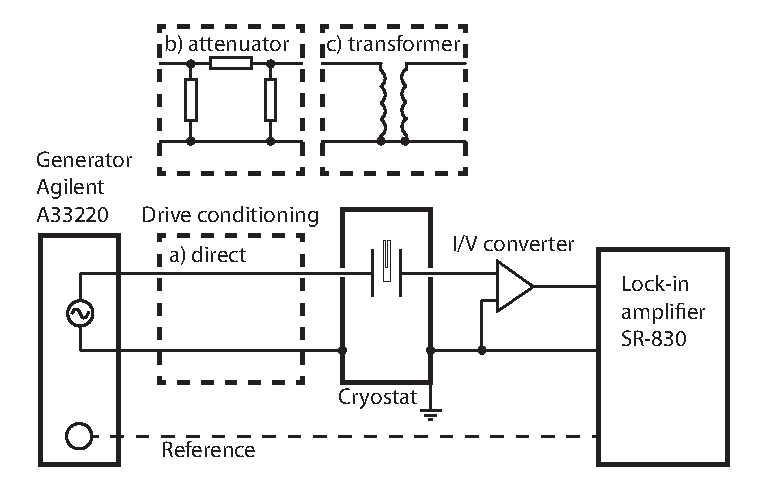
\includegraphics[width=0.6\textwidth]{graphics/exp/fork_setup}
	\caption{Diagram of the measurement scheme used in Prague. To achieve the full range of velocities, the applied voltage was either (a) directly fed to the tuning fork, (b) attenuated by one or more inline attenuators, or (c) amplified by a transformer. The transformer’s output was constantly monitored by a Keithley digital multimeter Model 2100. Source: \cite{multiple-vels}}
	\label{setup}
\end{figure}

\section{Measurement technique}

It was shown in previous works \cite{svoc2016} \cite{fork-exp}  with tuning forks submergend in Helium-II that it is important to perform full \textit{frequency sweeps} across the resonant response of an oscillator in order to reveal relevant details about any nonlinear effects.\\
However, these frequency sweeps, at fixed source drive, are heavily time-consuming and sometimes it is useful (especially when we are confident about present laminar mode) to use an \textit{amplitude sweep} with changing drives, a fixed resonant frequency.\\
Since many hydrodynamic features could be overlooked by using pure amplitude sweeps, we therefore focus in our analysis mainly on the frequency sweeps.


\newpage

%\chapter{Experimental Results}

In this chapter we present our obtained data and their analysis of the measurements from oscillatory experiments as introduced in \textbf{Experimental Approach} chapter.

In the first part, we present our drag force measurements by using all three oscillators submerged in superfluid Helium-II in hydrodynamical regime at temperatures $T > 1 \unit{K}$).

Next, we add measurements from the ballistic regime at temperatures $T < 0.6 \unit{K}$ abd connect them in order to prove the concept of universal scaling.

As the last analysis we introduce a \textit{flow phase diagram}, summarizing all our foundings basically in a single graph, representing the areas of different non-linear regimes.

\newpage

\section{Drag force measurements}

As we introduced in the last section of \textbf{Experimental approach} chapter, we used the full frequency sweep method for vibrating wire and tuning fork. Each point on following graphs was obtained by a pair of full frequency sweeps across the resonance of given oscillator. One sweep was performed with increasing frequency and the second one with decreasing frequency, which made us confident that no hysteresis effect was present.

We present all the measurements in the form of typical hydrodynamic visualizations (velocity-force response, drag coefficients and appropriate dimensionless numbers) of oscillating wire, torsional disc and tuning fork, respectively.

\subsection{Vibrating NbTi wire}

We were measuring both the voltage in-phase with the driving current and the quadrature signal, in order to obtain the resonant response. When a high enough applied drives were reached ($\gtrsim 0.8 \unit{mA}$ at temperature $1.67\unit{K}$, responding in $\sim 0.1 \unit{m/s}$ peak velocity), there was present a resonant frequency shift and a \textit{peak softening} effect.\\
As the calibration of the magnetic field produced by permanent magnets was performed only at room temperature, the peak velocity on the wire top is known with the accuracy about $\pm 20 \%$. This error doesn't affect the scaling process obtained from the data.

\begin{figure}[h]
	\centering
	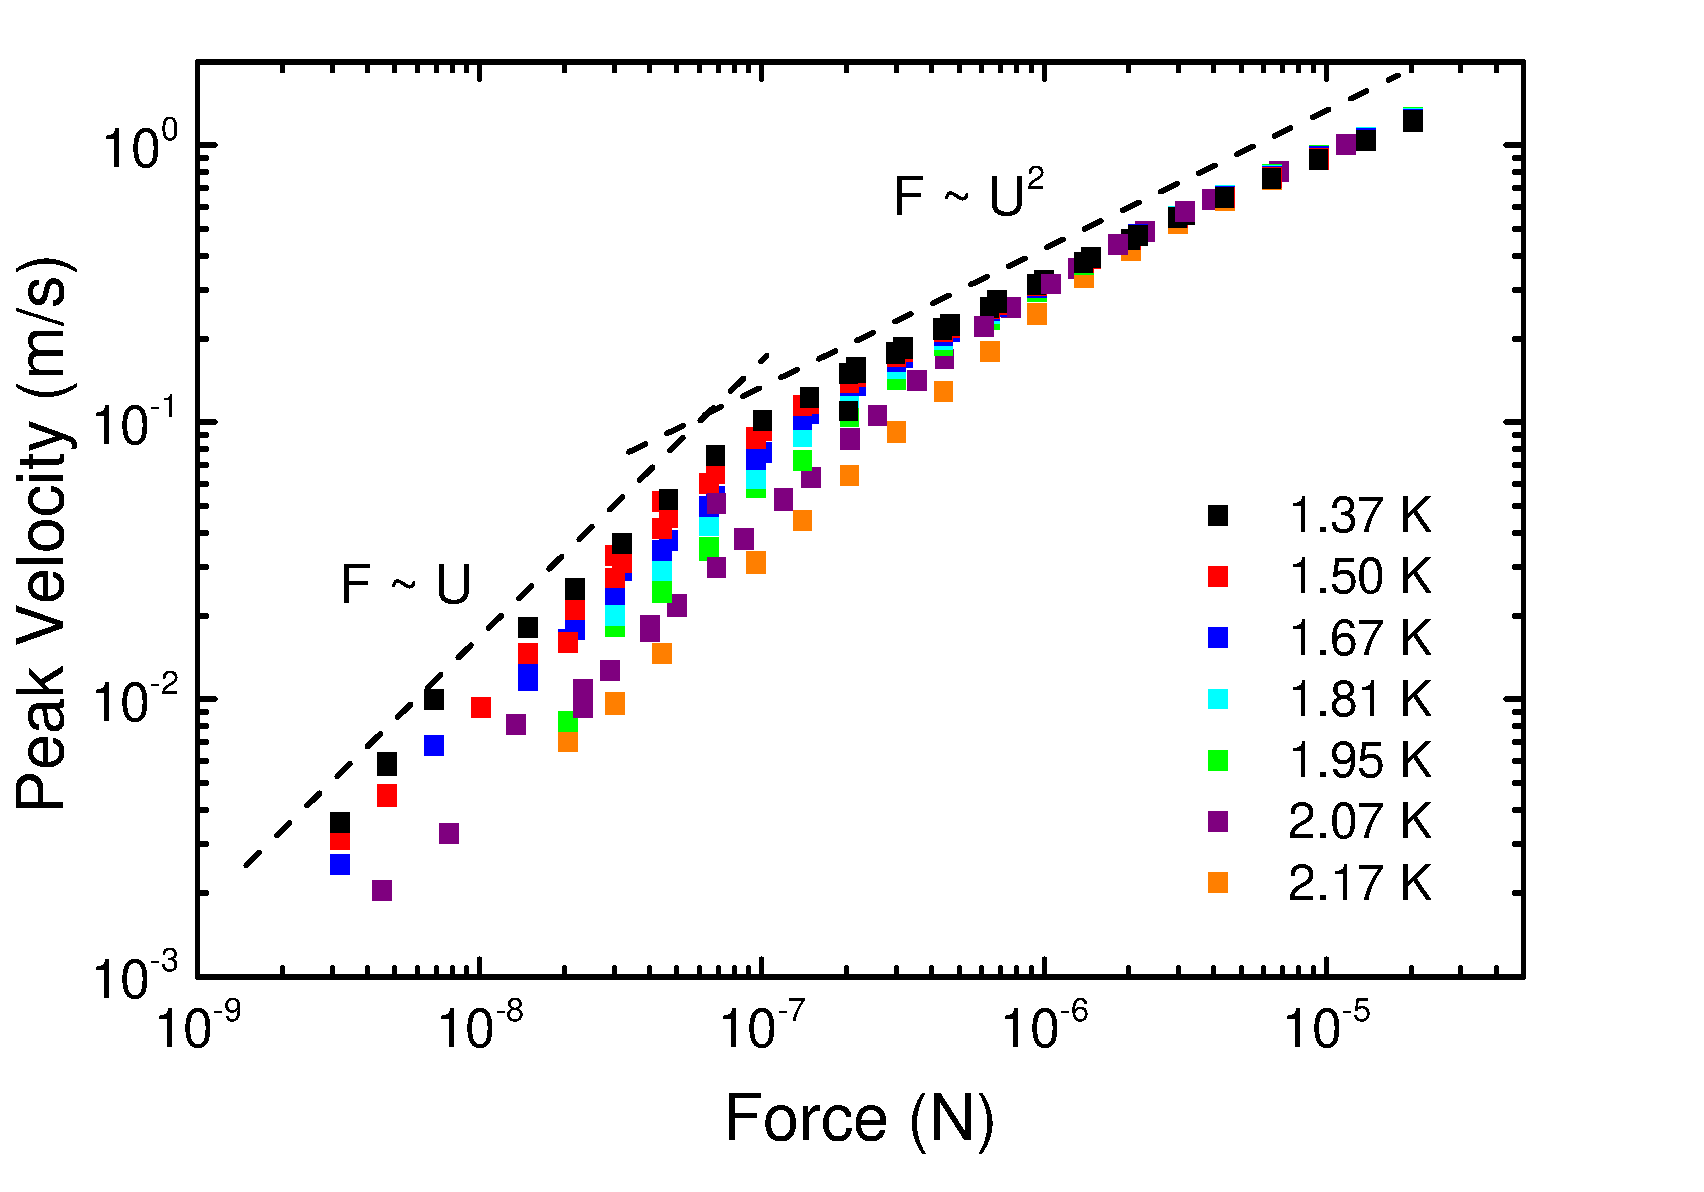
\includegraphics[width=0.7\textwidth]{graphics/results/wire_force_vel}
	\caption{Plot of peak velocity $U_0$ against the applied peak force $F_0$ for the vibrating wire submerged in superfluid $\He$ at several temperatures. The \underline{black dashed lines} serve as sketch of theoretical laminar and turbulent regimes.}
	\label{wire_vel_force}
\end{figure}

We plot in \textbf{Figure \ref{wire_vel_force}} the peak velocity of the wire top $U_0$ against the applied peak force $F_0$ at various temperatures from two-fluid regime ($T > 1.0\unit{K}$).

Clearly, the wire exhibits linear drag at low velocities and non-linear additional drag in the area of higher velocities. The energy losses of the wire in the low-velocity part are dominated by the viscous drag of the present normal component. Other loss mechanisms like acoustic emission are in principle present as well, but neglected in further discussion. The additional dissipation process in the higher-velocity part indicates either classical or quantum turbulence (or both) and the measured drag $F_0$ is roughly proportional to $U_0^2$.

Next we plot in \textbf{Figure \ref{wire_drag_vel}} the classical drag coefficient as a function of peak force and velocity $C_D \sim F_0 / U_0^2$ using the same data as presented in \textbf{Figure \ref{wire_vel_force}}.

\begin{figure}[h]
	\centering
	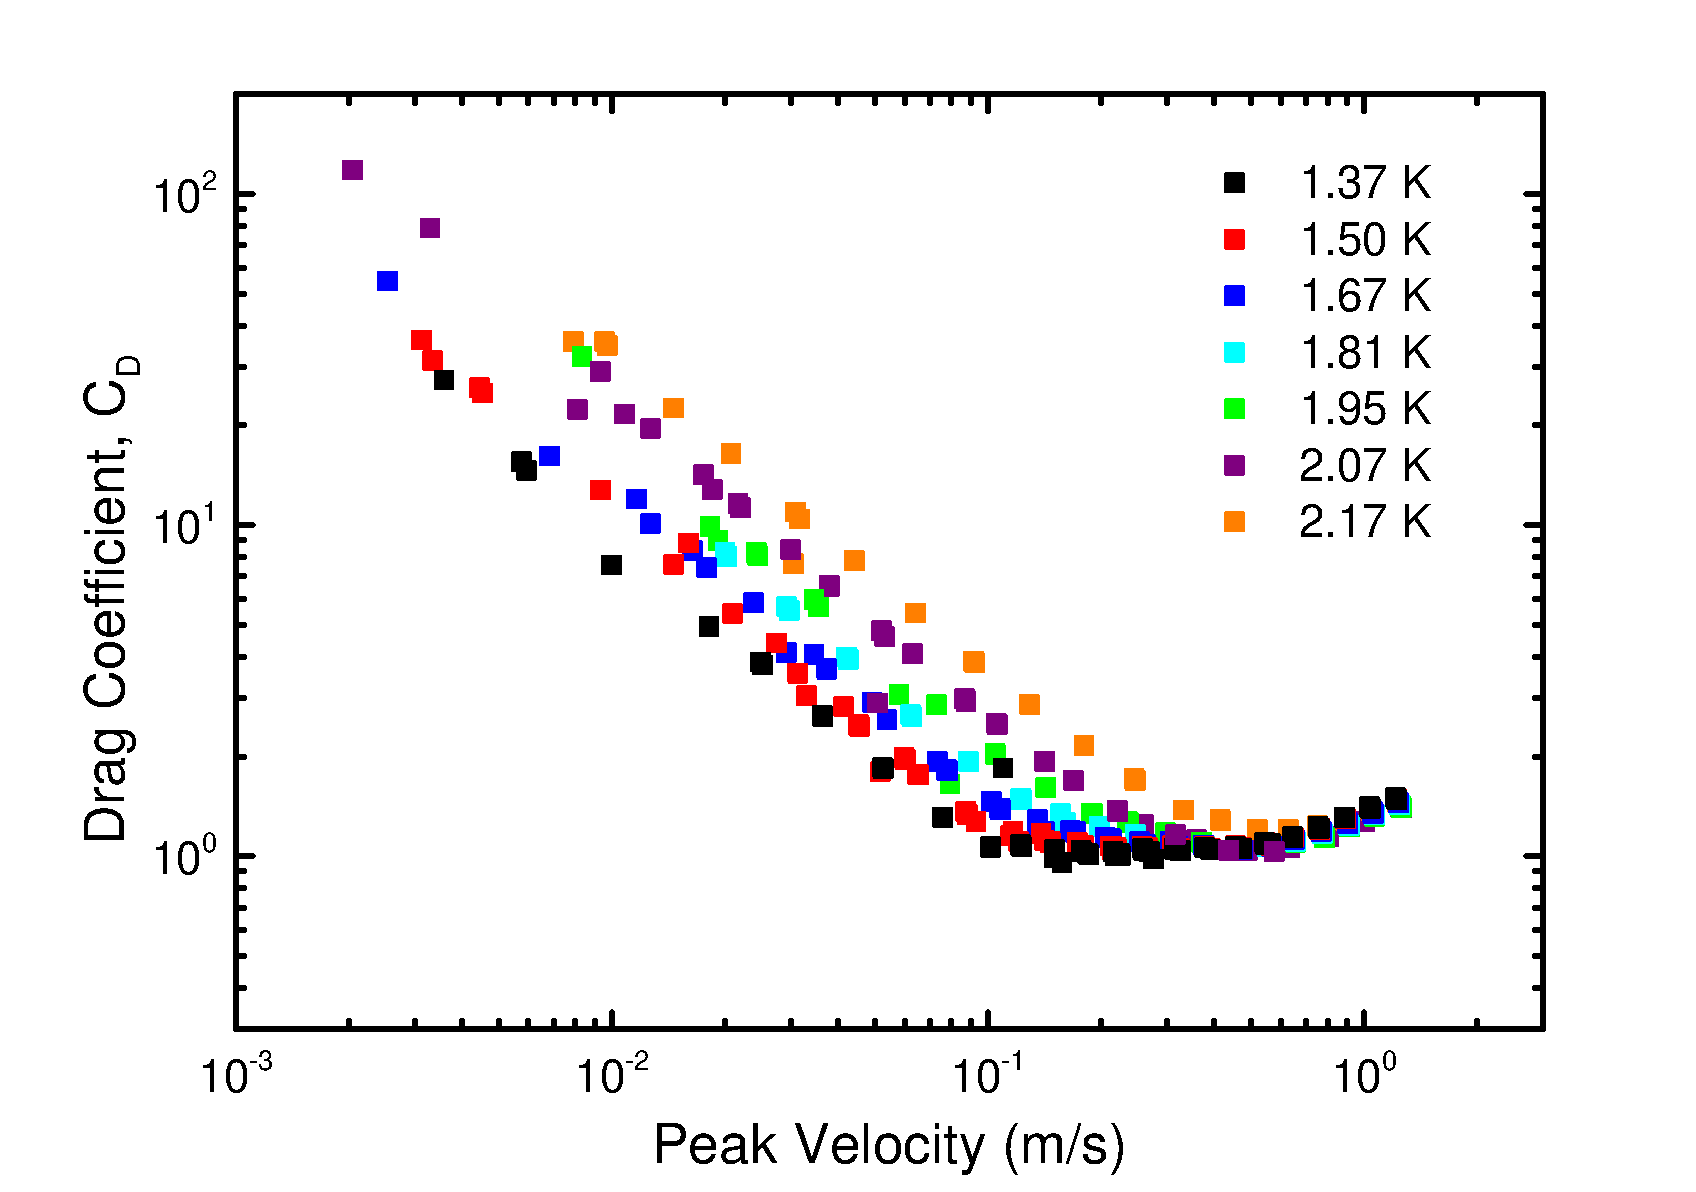
\includegraphics[width=0.7\textwidth]{graphics/results/wire_drag_vel}
	\caption{Plot of drag coefficient $C_D$ against the velocity peak response $U_0$ for the vibrating wire at several temperatures.}
	\label{wire_drag_vel}
\end{figure}

In order to perform the universal scaling, we collapse the contribution of the normal component in the following way:

\begin{equation}
C_D^{\,n} \leftarrow C_D \frac{\rho}{\rho_n}\,,
\hspace{1cm}
\text{Dn} \leftarrow U_0 \sqrt{\frac{2\rho_n}{\eta\omega}}\,,
\label{universal_scale}
\end{equation}

where $\eta$ is the dynamical viscosity of Helium-II for a given temperature. Relations in (\ref{universal_scale}) are applied in the same way as described (\ref{drag_normal}), (\ref{donnelly}) in the last section of \textbf{Theoretical background} chapter.\\
The resulting plot \textbf{Figure \ref{wire_drag_donnelly}} clearly shows the collapse of all linear parts of the measured drag into a single line. However, the theoretical pre-factor ($\Phi_{\text{cyl}} = 4\pi$) is smaller than the fitted one ($\Phi \sim 26$). This cannot be explained by experimental errors such as the magnet calibration, so the most likely reason behind it is the effect of irregularities on the surface of the wire. Indeed, excrescences of order $5 \mu\text{m}$ were observed on the $40 \mu \text{m}$ wire under an optical microscope.


\begin{figure}[h]
	\centering
	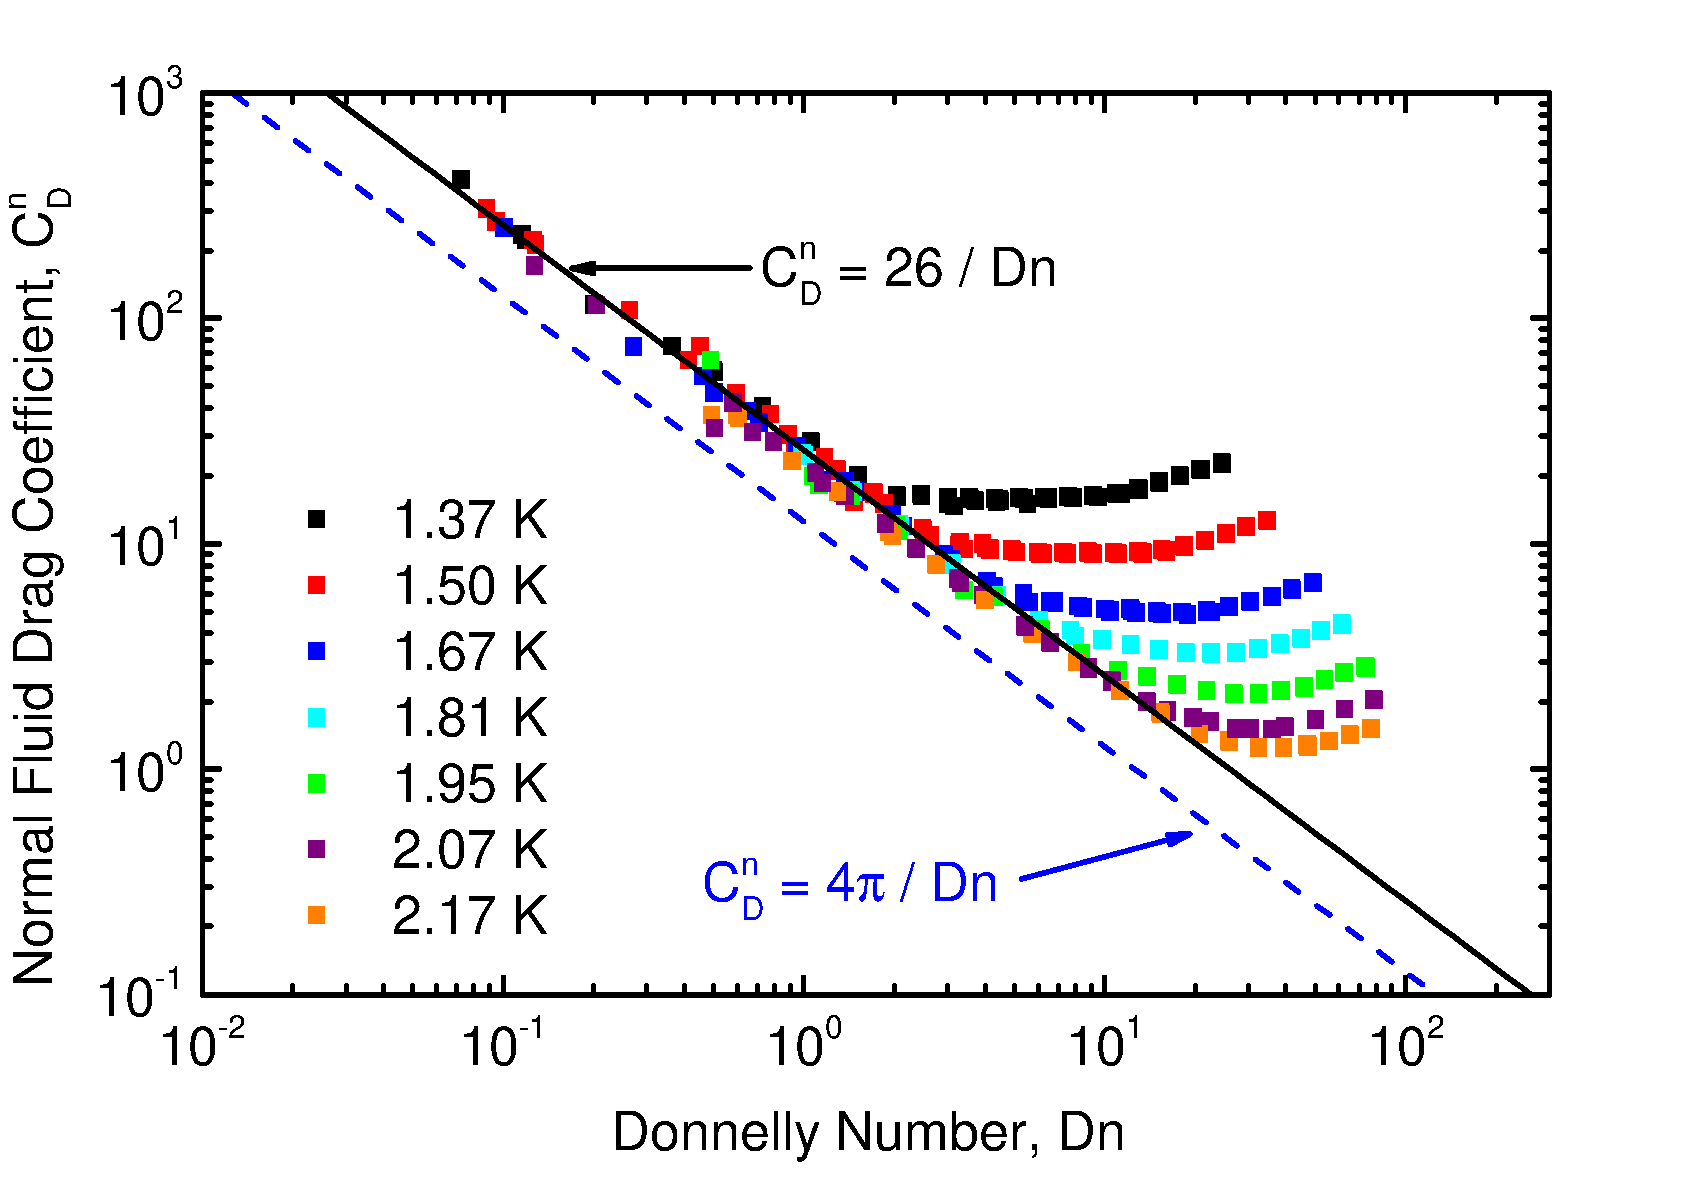
\includegraphics[width=0.7\textwidth]{graphics/results/wire_drag_donnelly}
	\caption{Plot of normal fluid drag coefficient $C_D^{\,n}$ against the dimensionless Donnelly number (Dn) for the vibrating wire at several temperatures.The \underline{blue dashed line} shows the expected theoretical dependence \cite{universal_scaling} for a smooth cylinder. The \underline{solid black line} is a numerical fit of the linear part of data.}
	\label{wire_drag_donnelly}
\end{figure}

One may see from the \textbf{Figure \ref{wire_drag_donnelly}} that all temperature curves are visually sorted ascendingly as the non-linear behaviour occurs at certain starting points. These points of non-linearity emergence cannot be governed by a single value of Donnelly number, but rather with a critical veloicity $U_C$.

We show in \textbf{Figure \ref{wire_nonlinear_drag}} that all deviations can be connected by the exceeding of critical dimensionless velocity $\hat{U}_C = U_C / \sqrt{\varkappa \omega}$. The approximate value of the critical $\hat{U}_C$ was found using \textit{error plot}, where the \textit{error} is defined via the absolutized errors of linear superfluid drag coefficient function $C_D^{\, s} = C_D \rho / \rho_s = \gamma / \hat{U}$:

\begin{equation}
\text{Error} = \frac{\text{abs}(C_D^{\,s} \hat{U} - \gamma)}{C_D^{\,s} \hat{U}} \in (0,1)\,,
\end{equation}

where $\gamma$ is the pre-factor coefficient, different for each temperature curve.

The single critical value $\hat{U}_C \sim 1$ (see \textbf{Figure \ref{wire_nonlinear_drag}}) is thus a clear sign of the onset of quantum turbulence by the superfluid component.

\begin{figure}[h]
	\centering
	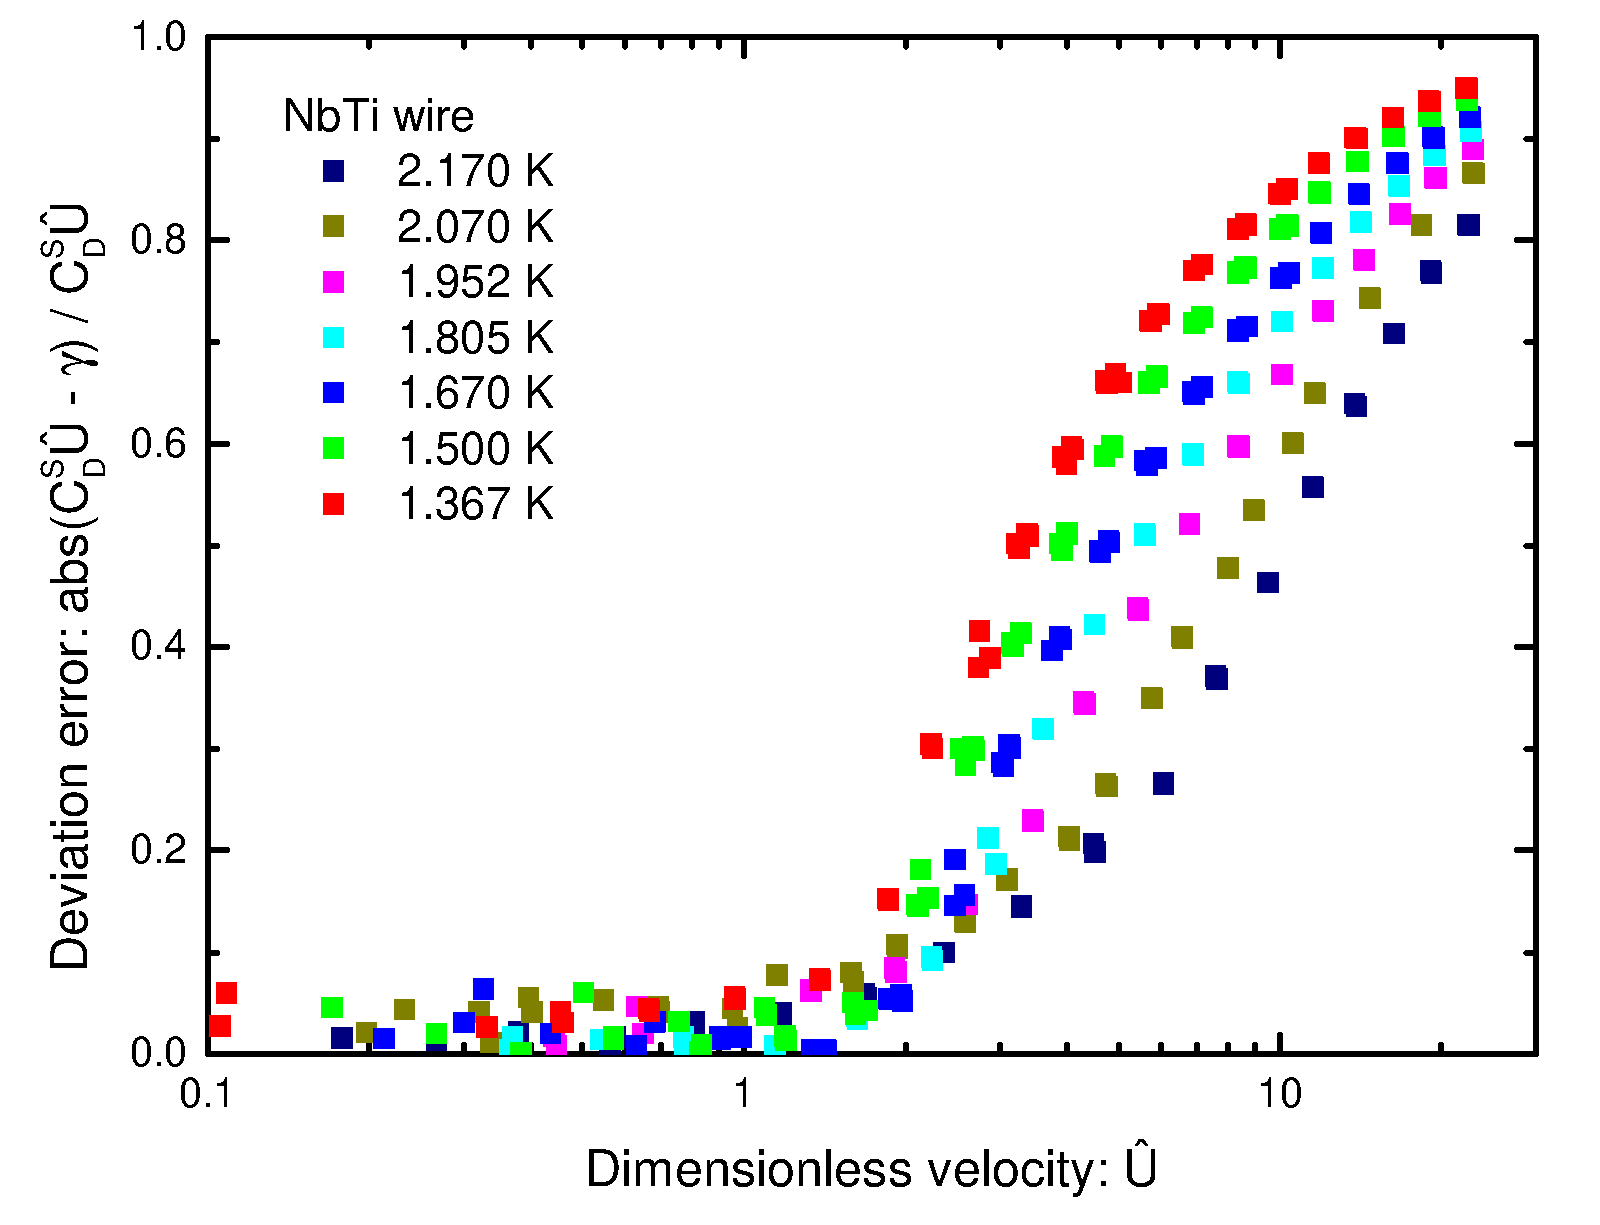
\includegraphics[width=0.7\textwidth]{graphics/results/wire_nonlinear_drag}
	\caption{Plot of normalized deviations from the linear fits $C_D^{\,s} =  \gamma / \hat{U}$ with $\gamma$ differing for each curve, as a function of the dimensionless velocity $\hat{U}$ for various temperatures from the studied range.}
	\label{wire_nonlinear_drag}
\end{figure}


%%%%%%%%%%%%%%%%%%%%%%%%%%%%%%%%%%%%%%%%%%%%%%%%%%%%%%%%%%%%%%%%%%%%%%%%%%%%%%%%%%%%%%%

\subsection{Oscillating disc}

The (torsionally) oscillating disc differs from the vibrating wire in several technicalities:

\begin{itemize}
  \item Oscillating disc does not displace any fluid and thus The superfluid is at rest unless quantized vorticity is produced
  \item It is not possible to perform measurements in a steady state of flow, but decayed flow was measured instead
  \item Drag force has to be inferred from the decaying amplitude of oscillator deflection.
\end{itemize}

As a consequence of mentioned differences (examples showed in \textbf{Figure \ref{disc_extrema}}), we have to substitute $U_0 = \omega R \phi_0$ within the Donnelly number and define a new drag coefficient, specific for our mechanical system of torsionally oscillating disc in a viscous fluid of density $\rho_n$ as:
\begin{equation}
C_D^{\,n} \leftarrow \frac{2M_f}{A\rho_n \Omega_0^2 R^3}\,,
\hspace{1cm}
\text{Dn} \leftarrow R\omega \phi_0 \sqrt{\frac{2\rho_n}{\eta\omega}}\,,
\label{disc_scale}
\end{equation}

where $M_f$ is the moment of friction forces, $R$ the radius of the disc, $A = \pi R^2$ the area of the disc and $\Omega_0$ is the amplitude of angular frequency $\omega(t)$. It was already showed \cite{universal_scaling} the relation between such drag coefficient (\ref{disc_scale}) can be expressed in laminar flow in terms of the Donnelly number as $C_D^{\,n} = \Phi /\text{Dn}$ with the pre-factor $\Phi_{\text{disc}} = 2$.

\begin{figure}[h]
	\centering
  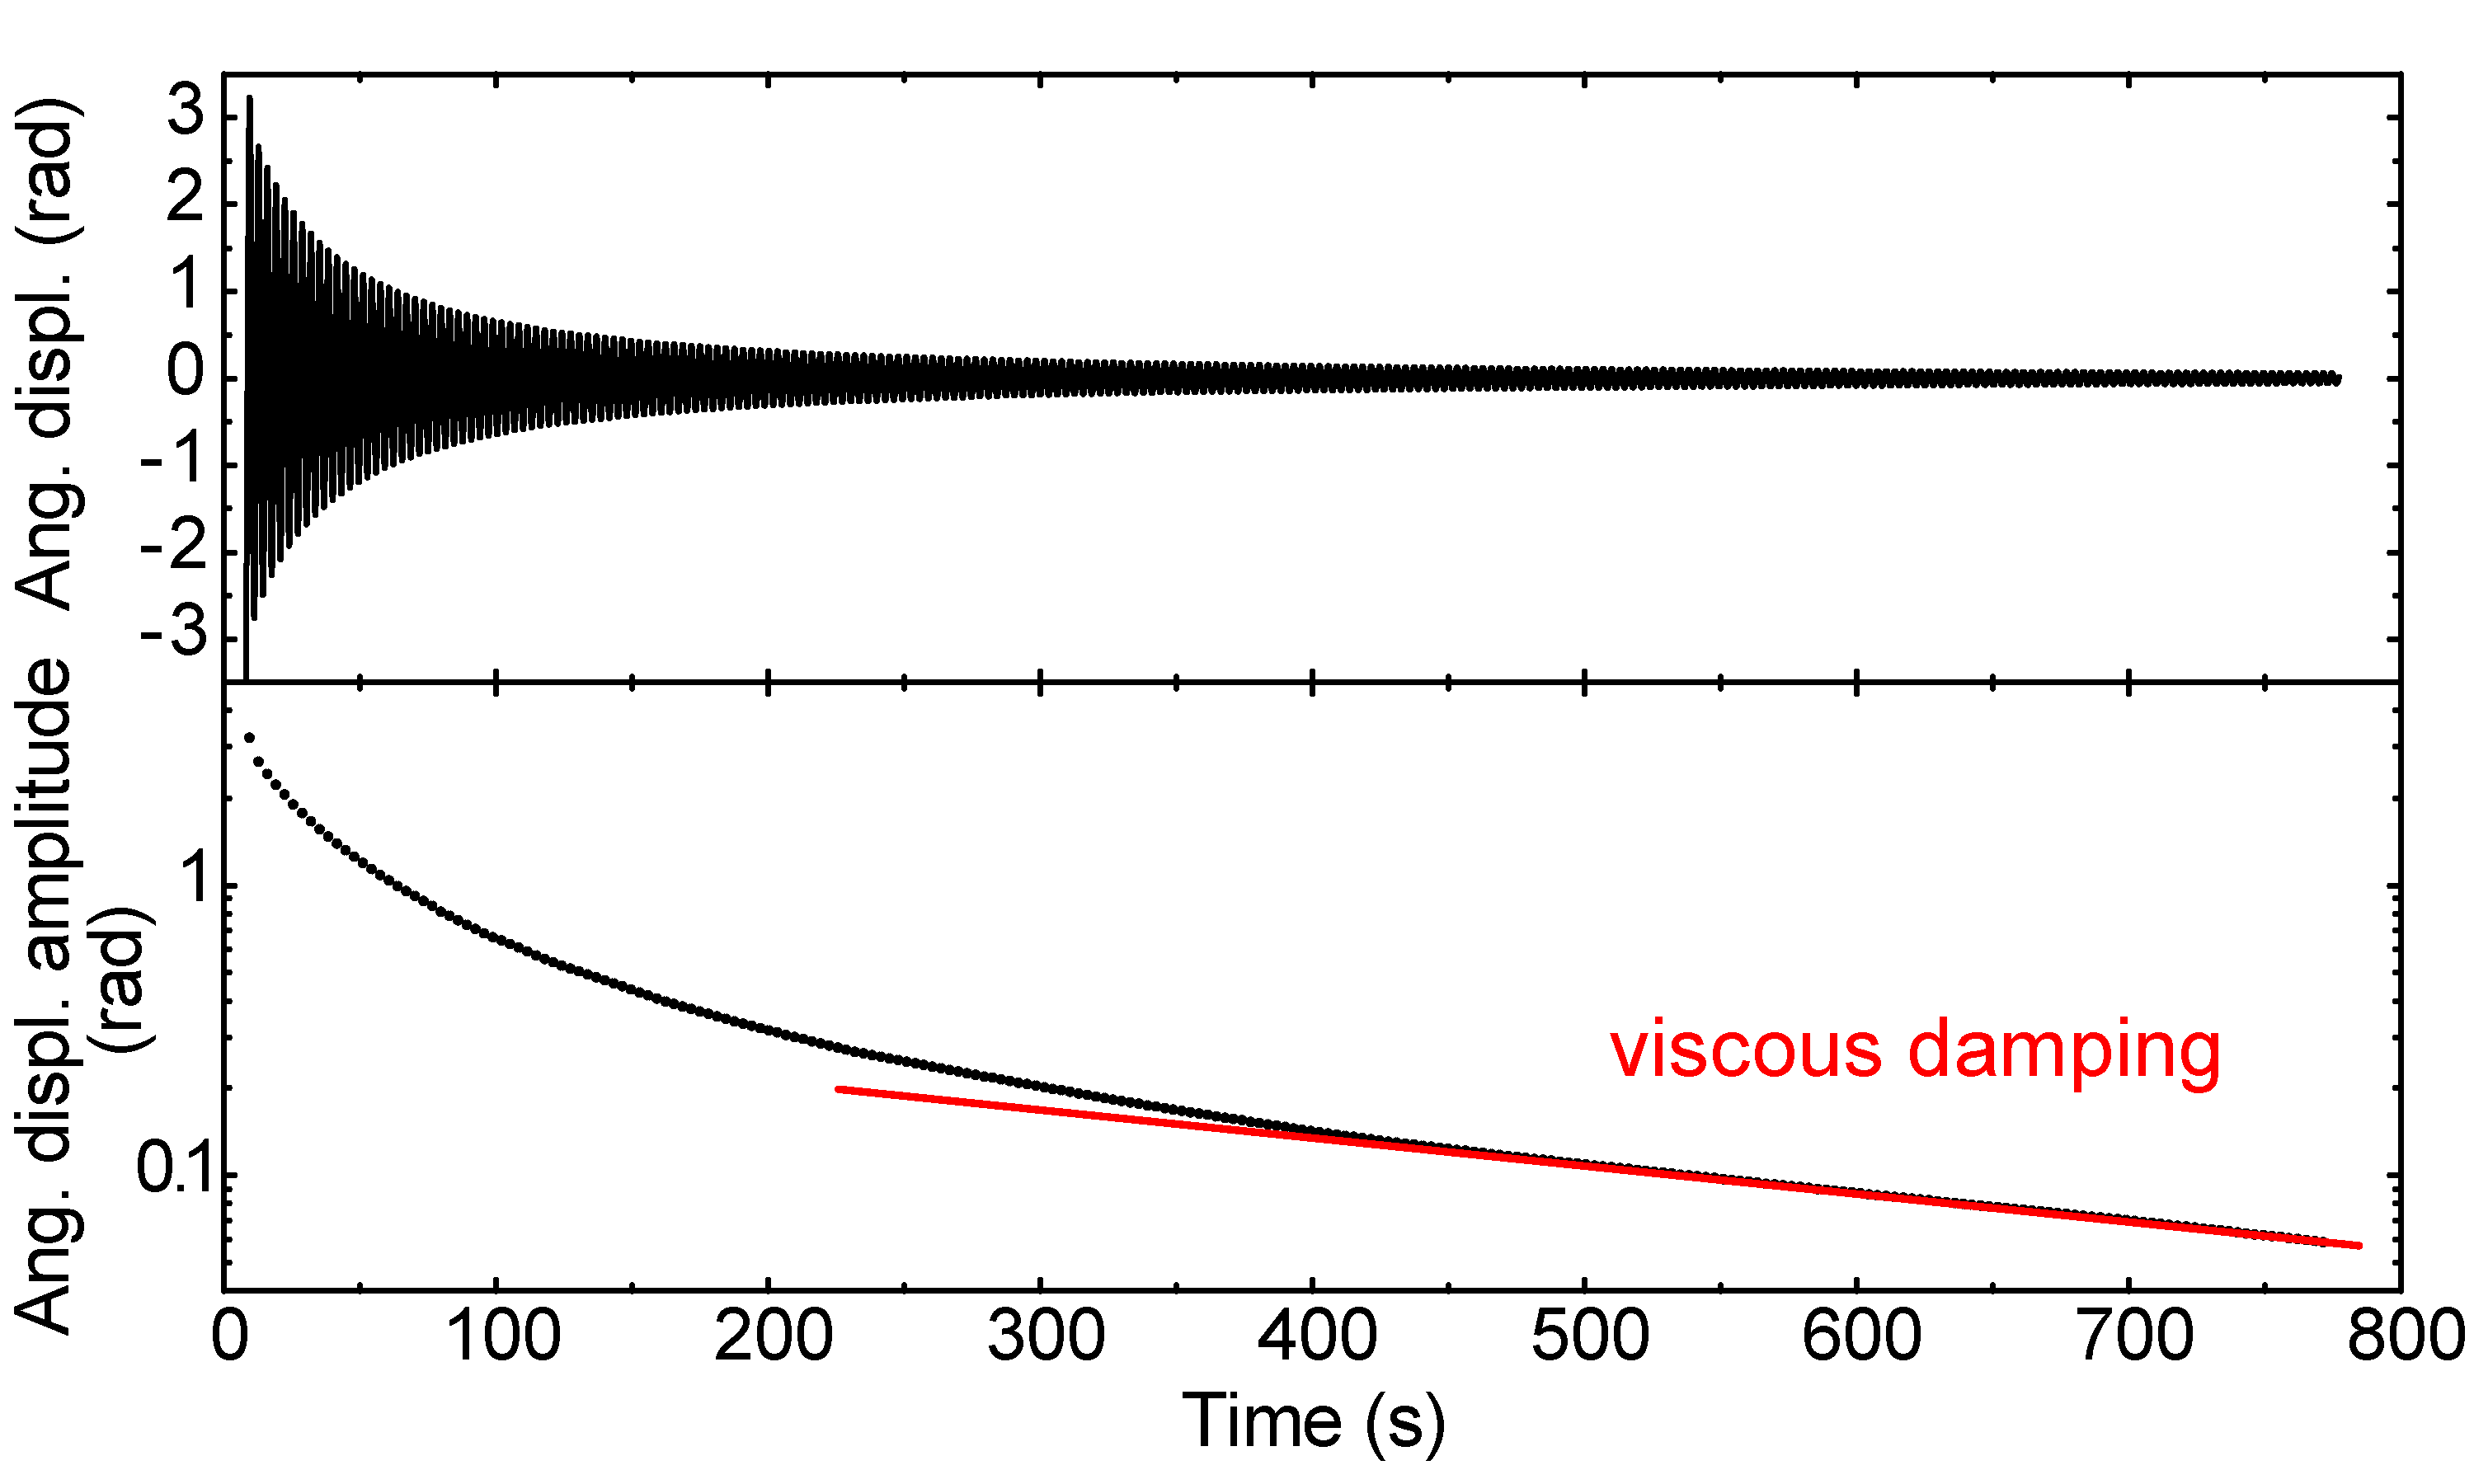
\includegraphics[width=0.8\textwidth]{graphics/results/disc_extrema}
  \caption{Example of angular displacement measurement in time of the torsionally oscillating disc.\\
  \underline{Top picture:} The decreasing angular displacement amplitudes $\phi_0 (t)$.
  \underline{Bottom picture:} The logarithmic plot $\phi_0 (t)$ shows two distinct regions – nonlinear decay in the area of earlier times $t < 400$ due to turbulent drag forces and an exponential (viscous) decay due to laminar flow of the normal component at the later times $t > 500$.}
  \label{disc_extrema}
\end{figure}

We plot the re-defined drag coefficient $C_D^{\,n}$ (\ref{disc_scale}) against the Donnelly number in \textbf{Figure \ref{disc_drag_donnelly}}.
Again, as in case of vibratig wire, the data collapse to a single inverse dependence $C_D^{\,n} = 2 / \text{Dn}$ in the area of small values of Donnelly number, which illustrates and proves the universal scaling concept.\\
One would naturally expect the normal component to transit to turbulent regime earlier than the superfluid one since the oscillating disc directly moves only with the normal component. However, \textbf{Figure \ref{disc_drag_donnelly}} clearly shows that non-linearities are not characterized by a single value of Dn, but rather continuously with ascending temperature. This implies that instabilities cannot be explained by pure viscous fluid dynamics and must relate to the quantum turbulence produced by a Donnelly-Glaberson instability.

We don't provide the error plot for this oscillator since it looks practically identical to the one presented with vibrating wire and brings no additional information. The critical dimensionless velocity of the torsionally oscillating disc is estimated (from the error plot) as $\hat{U}_C \sim 12$. This is about one order higher than in the case of vibrating wire.

\newpage

\begin{figure}[h]
	\centering
  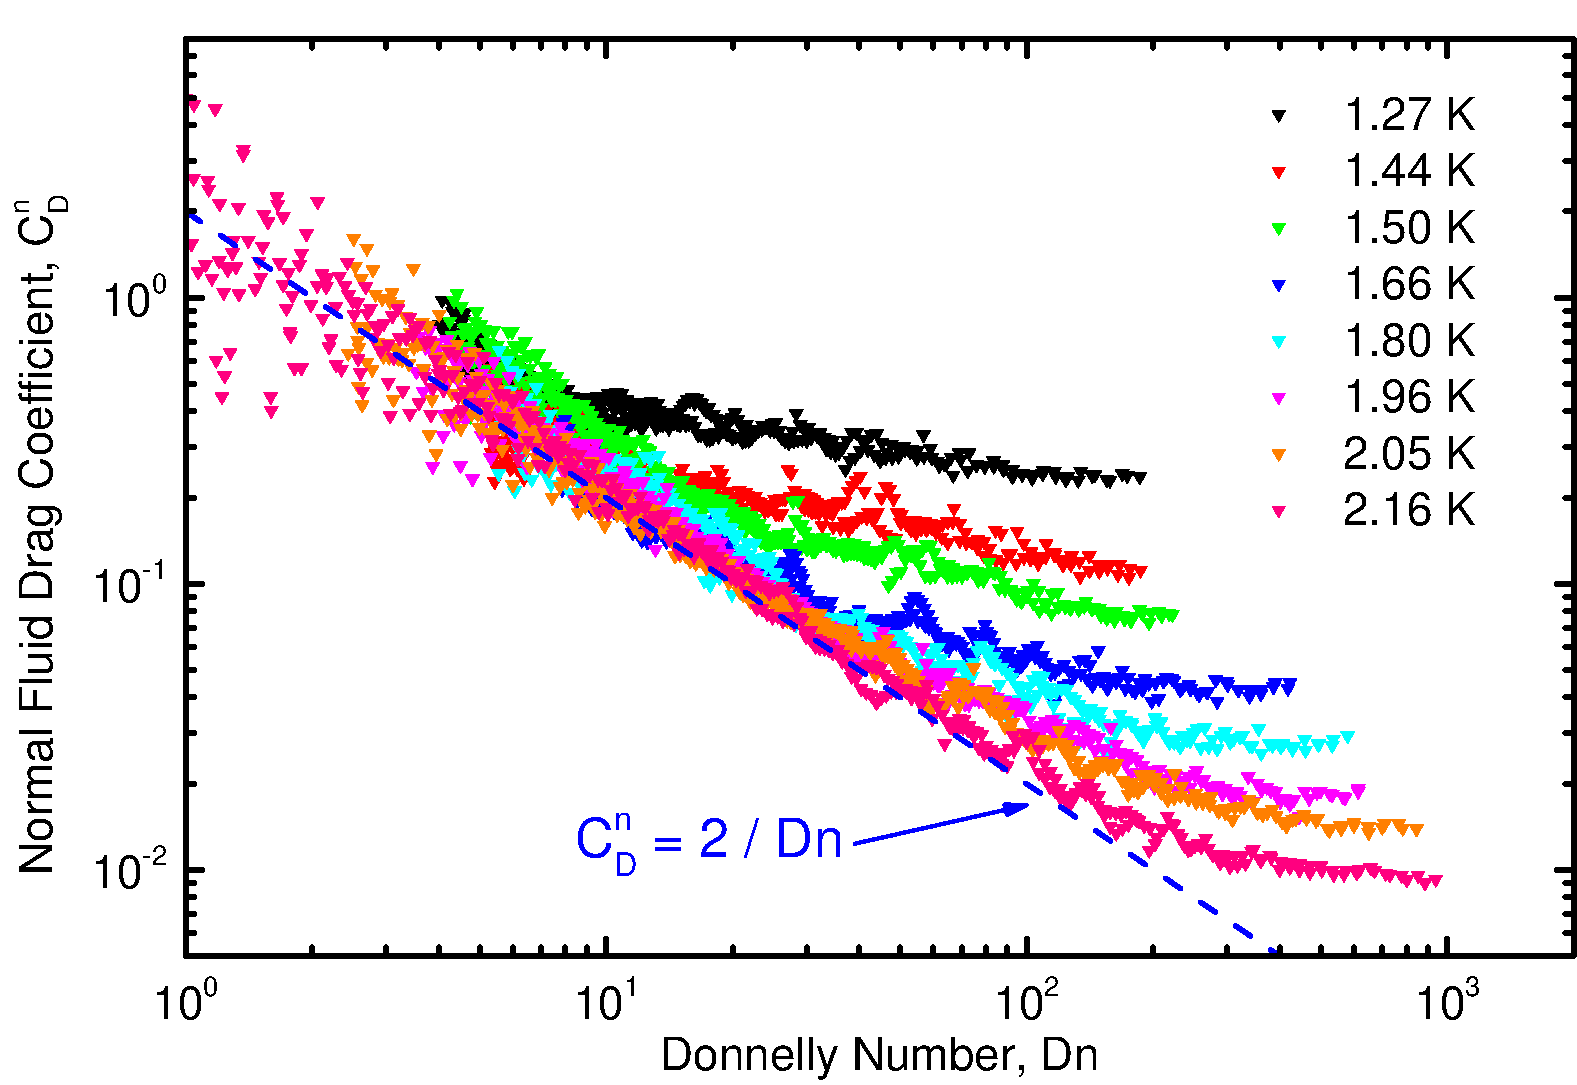
\includegraphics[width=0.7\textwidth]{graphics/results/disc_drag_donnelly}
  \caption{Plot of re-defined fluid drag coefficient $C_D^{\,n}$ against the dimensionless Donnelly number (Dn) for the torsionally oscillating disc at several temperatures.\\
  The \underline{blue dashed line} shows the expected theoretical dependence \cite{universal_scaling} for viscous drag. The temperature-dependent and temperature-ascending starting points of non-linearities are a clear sign of the onset of quantum turbulence by the superfluid component.}
  \label{disc_drag_donnelly}
\end{figure}


%%%%%%%%%%%%%%%%%%%%%%%%%%%%%%%%%%%%%%%%%%%%%%%%%%%%%%%%%%%%%%%%%%%%%%%%%%%%%%%%%%%%%%%%%%

\subsection{Tuning fork}

As the last oscillator, we used quartz tuning fork with geometry and resonant specifics as they were described in \textbf{Experimental approach} chapter. the resonant response was experimentally measured in the same way as was with vibrating wire - by a real-time analysis of the in-phase current and quadrature response. Electrical quantities are then converted into physical attributes according to mentioned relations (\ref{fork_conversions}), which are dependent on fork constants $a_{f0} = 3.665 \times 10^{-7} \unit{Cm}^{-1}$, $a_{f1} = 14.094 \times 10^{-7} \unit{Cm}^{-1}$ for the fundamental and overtone mode, respectively. \\
In order to measure the fork constants, we had to perform a series of frequency sweeps in low-temperature vacuum. We estimate the uncertainty of fork constants to be of $10\%$ since velocity calculation errors were proven using optical experiments. \cite{optical_exps}

\newpage

In \textbf{Figure \ref{fork-vel_force}} we plot the peak velocity response $U_0$ of the top of the fork prong, against the applied peak force $F_0$ at various temperatures from two-fluid regime ($T > 1.0\unit{K}$). We sketched the theoretical laminar $F_0 \propto U_0$ and classical turbulent dependencies $F_0 \propto U_0^2$ as guides for the eye.

\begin{figure}[h]
	% \centering
	\hspace{-1.7cm}
	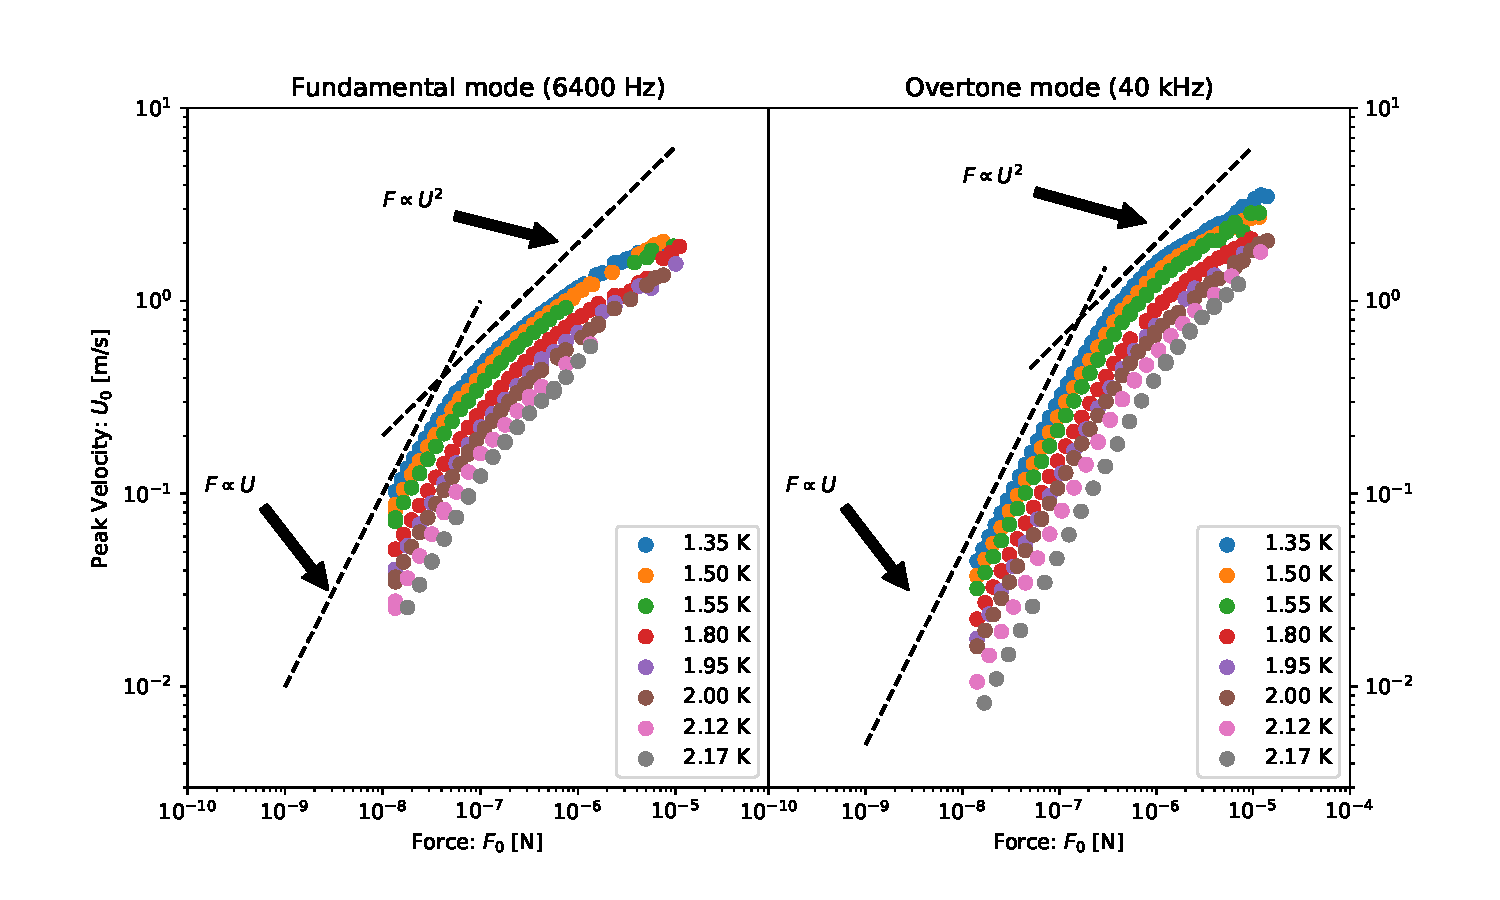
\includegraphics[width=1.2\textwidth]{graphics/results/fork-vel_force}
	\caption{Plot of peak velocity $U_0$ against the applied peak force $F_0$ for the oscillating tuning fork submerged in superfluid $\He$ at several temperatures.\\
	\underline{Left image:} Measurements in fork's fundamental mode, \underline{Right image:} Measurements in fork's overtone mode, \underline{Black dashed lines} mark the theoretical laminar and classical turbulent regime dependencies.}
	\label{fork-vel_force}
\end{figure}

We note that the linear sketched dependency decribe the laminar regime very well, whereas the quadratical (classical turbulence regime) seems to be a weak fit to the situation, especially for the lower temperatures from the studied range.

Next, we plot in \textbf{Figure \ref{fork-drag_vel}} the classical drag coefficient $C_D$ against the peak velocity $U_0$. Both oscillating modes are visualised as a paired plot in order to show their shared asymptote (as sketched with the black dashed line) in the area of big velocities. Also, we sketched the laminar regime fit as a demonstration.

\newpage

\begin{figure}[h]
	% \centering
	\hspace{-1.7cm}
	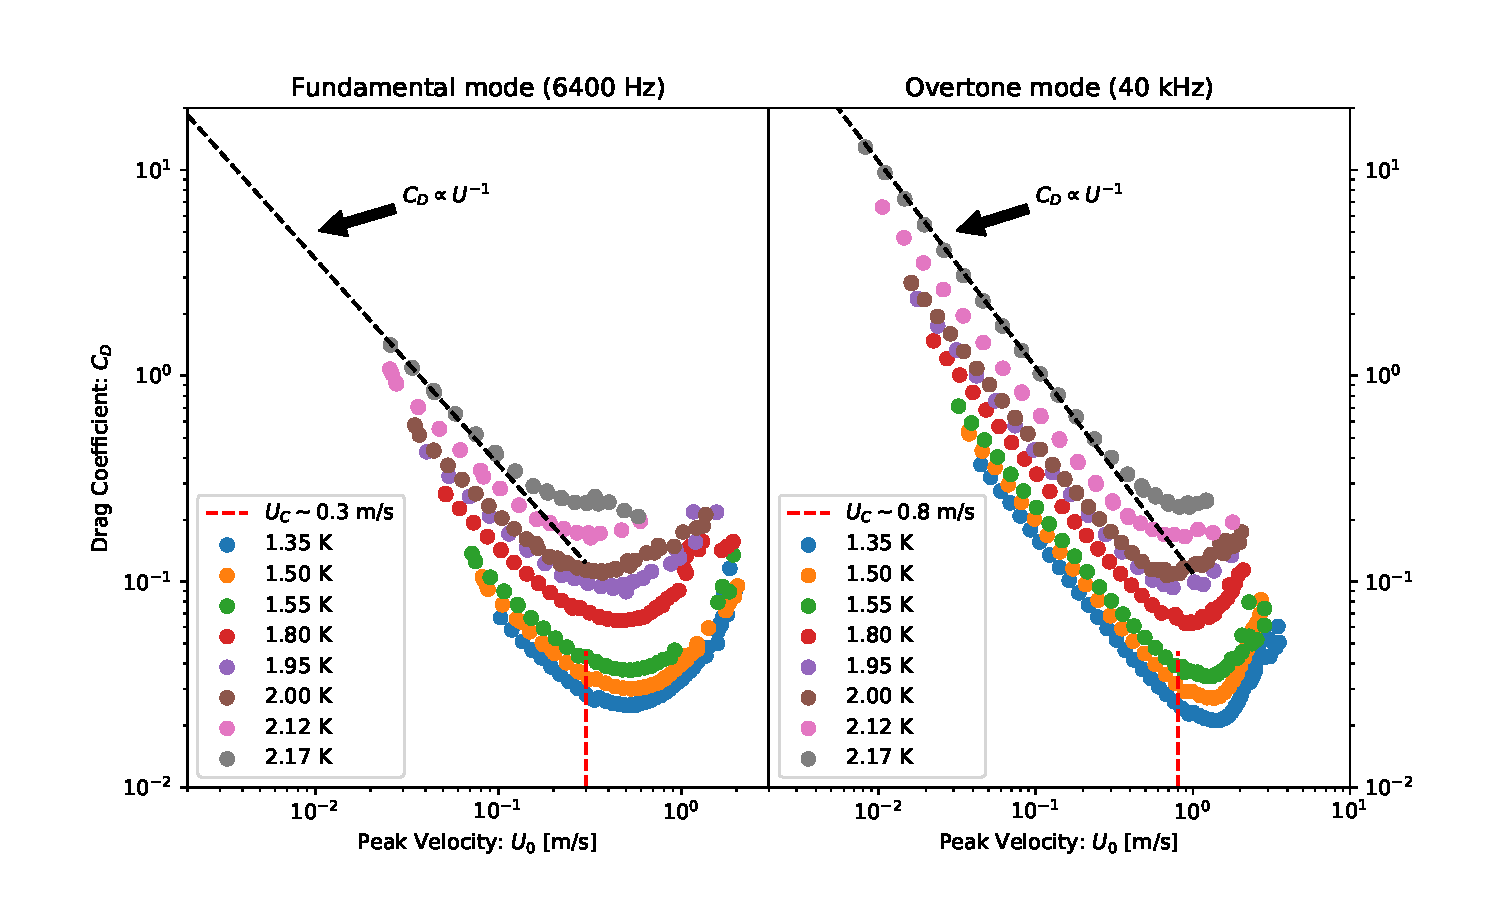
\includegraphics[width=1.2\textwidth]{graphics/results/fork-drag_vel}
	\caption{Plot of drag coefficient $C_D$ against the velocity peak response $U_0$ for the oscillating tuning fork submerged in superfluid $\He$ at several temperatures.\\
	\underline{Left image:} Measurements in fork's fundamental mode, \underline{Right image:} Measurements in fork's overtone mode, \underline{black dashed line} fits the theoretical laminar regime dependency, \underline{red dashed line} marks the critical velocity value $U_C$ above which an onset of quantum turbulence appears. The clear sign of this effect can be seen for a group of curves with $T < 1.6\unit{K}$.}
	\label{fork-drag_vel}
\end{figure}

As expected, the tuning fork exhibits a linear drag in the area of low velocities regardless on the temperature from the studied range. Then, approximately above the critical velocity $U_C$, a synchronized increased drag was observed for a group of curves with temperature $T < 1.6\unit{K}$, which is a clear sign of onset of quantum turbulence. The critical velocities differ for oscillating modes:

\begin{equation}
U_{C0} \sim 0.3 \unit {m/s}
\hspace{1cm}
U_{C1} \sim 0.8 \unit {m/s}\,,
\end{equation}

which is expected from the scaling relation (\ref{drag_super}) and roughly proven since the critical dimensionless velocities $\hat{U}_{C0} = U_{C0} / \sqrt{ \varkappa \omega_0} \approx 4.7$ and $\hat{U}_{C1} = U_{C1} / \sqrt{ \varkappa \omega_1} \approx 5.0$ are similar.

Curves with higher temperature seem to transit to non-linear regime earlier, which indicates the classical turbulence of the normal component instead.

\newpage

To characterize the normal component flow, we plot in \textbf{Figure \ref{fork-drag_donnelly}} the normal drag coefficient against the dimensionless Donnelly number. The conversions were done as we stated in (\ref{universal_scale}).

\begin{figure}[h]
	% \centering
	\hspace{-1.7cm}
	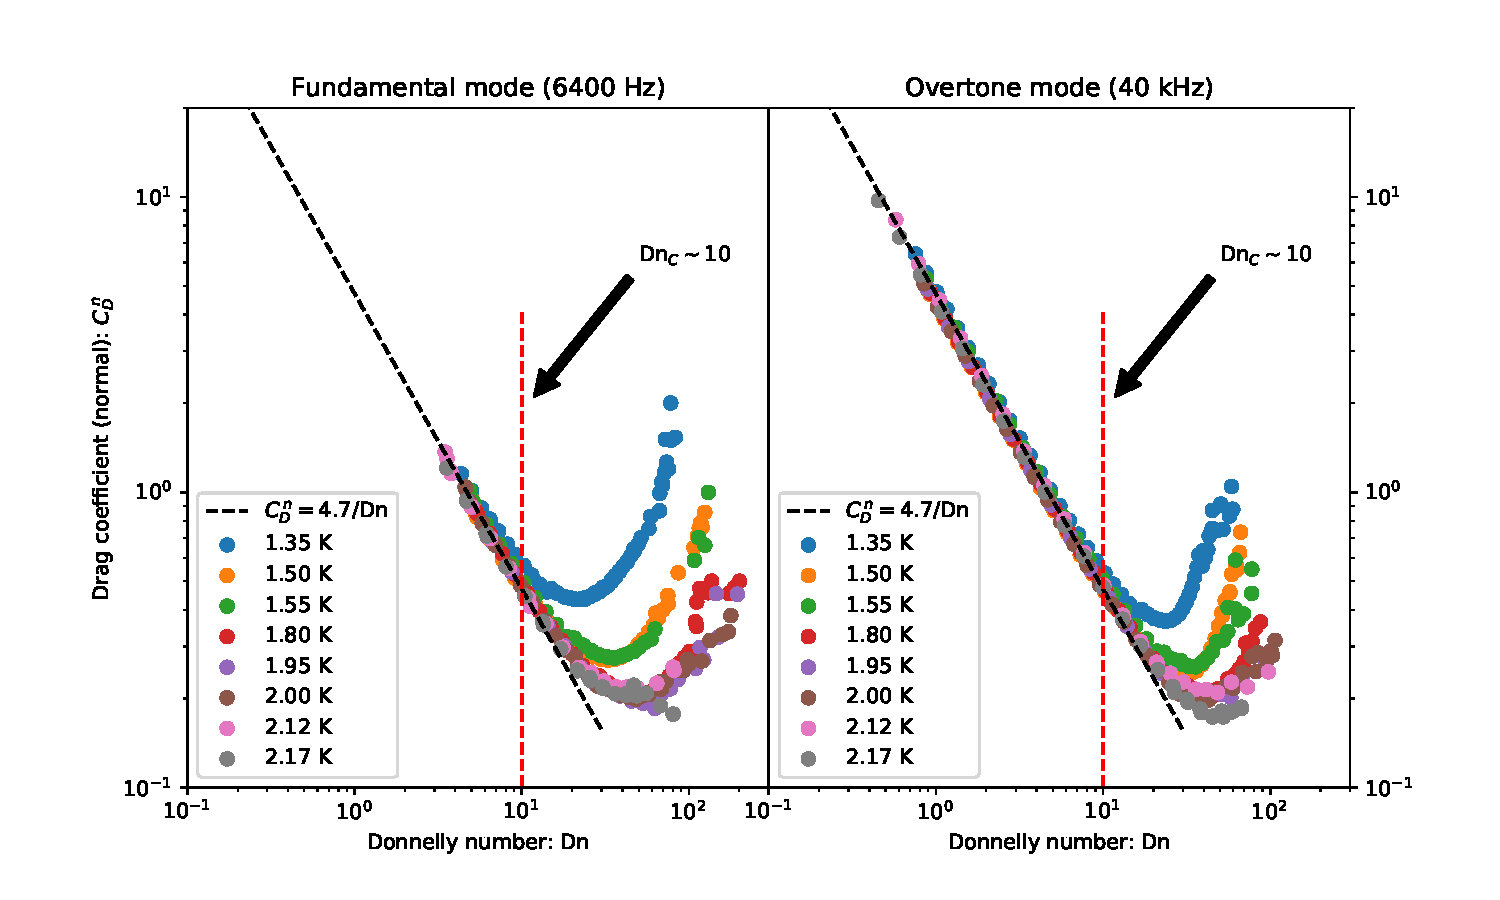
\includegraphics[width=1.2\textwidth]{graphics/results/fork-drag_donnelly}
	\caption{Normal fluid drag coefficient $C_D^{\,n}$ as a function of the Donnelly number Dn. \underline{Left image:} Measurements in fork's fundamental mode, \underline{Right image:} Measurements in fork's overtone mode, \underline{Black dashed line} fits the theoretical laminar regime dependency, with the same pre-factor $C_D^{\,n} = 4.7 / \text{Dn}$ for both oscillation modes, \underline{Red dashed line:} the estimated critical value of Dn, above which the onset of classical turbulence occurs for the group of temperature curves $T > 1.6 \unit{K}$.}
	\label{fork-drag_donnelly}
\end{figure}

With no doubt, in the area of low Donnelly values, the dependencies collapse to a single line as expected, representing the laminar regime with the shared pre-factor $\Phi \sim 4.7$. In contrast to the results obtained with the vibrating wire or oscillating disc, we also recognize, additionally to the critical velocity $\hat{U}_C$, a critical value of Donnelly number $\text{Dn}_C$, above which the rest group of temperature curves $T > 1.6\unit{K}$ non-linearly deviate.
The onset of turbulence for these curves is governed by a single value of Donnelly number $\text{Dn}_C$ and thus dominated by the classical turbulence of the normal component.\\
We note that it is interesting to find the laminar pre-factor $\Phi \sim 4.7$ to be same for both oscillation modes. The shared critical $\text{Dn}_C$ was expected from the dynamical similarity principle, but the shared $\Phi$ is a result of different principle - the fact that both modes have the same effective mass $m_{\text{eff}}$ (see \cite{universal_scaling}).

\newpage

We found the approximate value for the shared critical Donnelly number $\text{Dn}_C$ again using \textit{error plot}, where the \textit{error} is here defined via the normalized deviation rate from the laminar fit $f: C_D^{\,n} \text{Dn} - \Phi$, where $\Phi = 4.7$ as:

\begin{equation}
\text{Error} = \frac{\text{abs}(C_D^{\,n} \text{Dn} - \Phi)}{C_D^{\,n}\text{Dn}} \in (0,1)
\end{equation}

We plot these errors in \textbf{Figure \ref{fork-error_donnelly}} in order to mark more clearly the position of $\text{Dn}_C$, where the group of temperatures $T > 1.6\unit{K}$ starts to deviate.

\begin{figure}[h]
	% \centering
	\hspace{-1.7cm}
	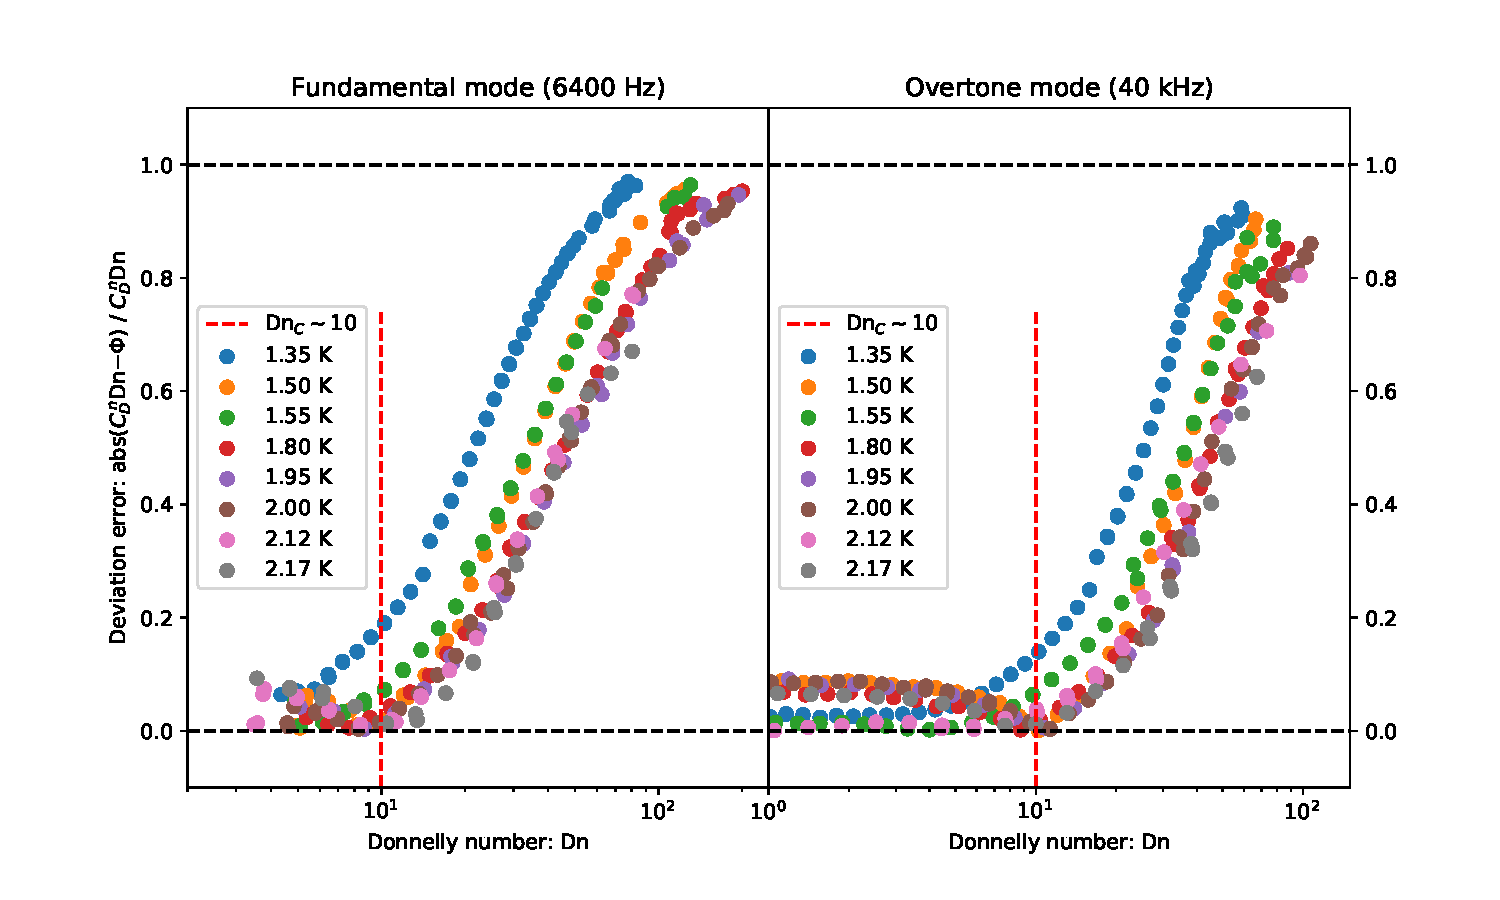
\includegraphics[width=1.2\textwidth]{graphics/results/fork-error_donnelly}
	\caption{Plot of normalized deviations from the linear fit $C_D^{\,n} =  \Phi / \text{Dn}$ with $\Phi = 4.7$ as a function of the Donnelly number. \underline{Left image:} Errors in fork's fundamental mode, \underline{Right image:} Errors in fork's overtone mode, \underline{Black dashed lines} mark the boundaries and \underline{red dashed lines} our estimations for the values of Dn${}_C$.
	}
	\label{fork-error_donnelly}
\end{figure}

Our estimated value for critical Donnelly number $\text{Dn}_C$ for temperature curves $T > 1.6\unit{K}$ and for both oscillation modes is $\text{Dn}_C \sim 10$. This shared value of $\text{Dn}_C$ proves the high-frequency regime validity and thus the possible domination of classical turbulence from normal component.

\section{Ballistic regime}

In this section, we demonstrate the limits of universal scaling validity. In \textbf{Figure \ref{ballistic}} we plot the scaling function of Weissenberg number $f(\text{Wi})$, as derived in \cite{scaling_function} and introduced in the \textbf{Theoretical Background} in (\ref{scaling_function}). In order to validate the derivation, we add the experimental results obtained with a tuning fork in two-fluid regime (presented in previous section) and also in ballistic regime ($T < 0.6\unit{K}$).
Again, these regimes represent the Newtonian hydrodynamics ($\text{Wi} \ll 1$), governed by Navier-Stokes equations, and a non-newtonian gas dynamics. \cite{universal_scaling}

\begin{figure}[h]
	\centering
	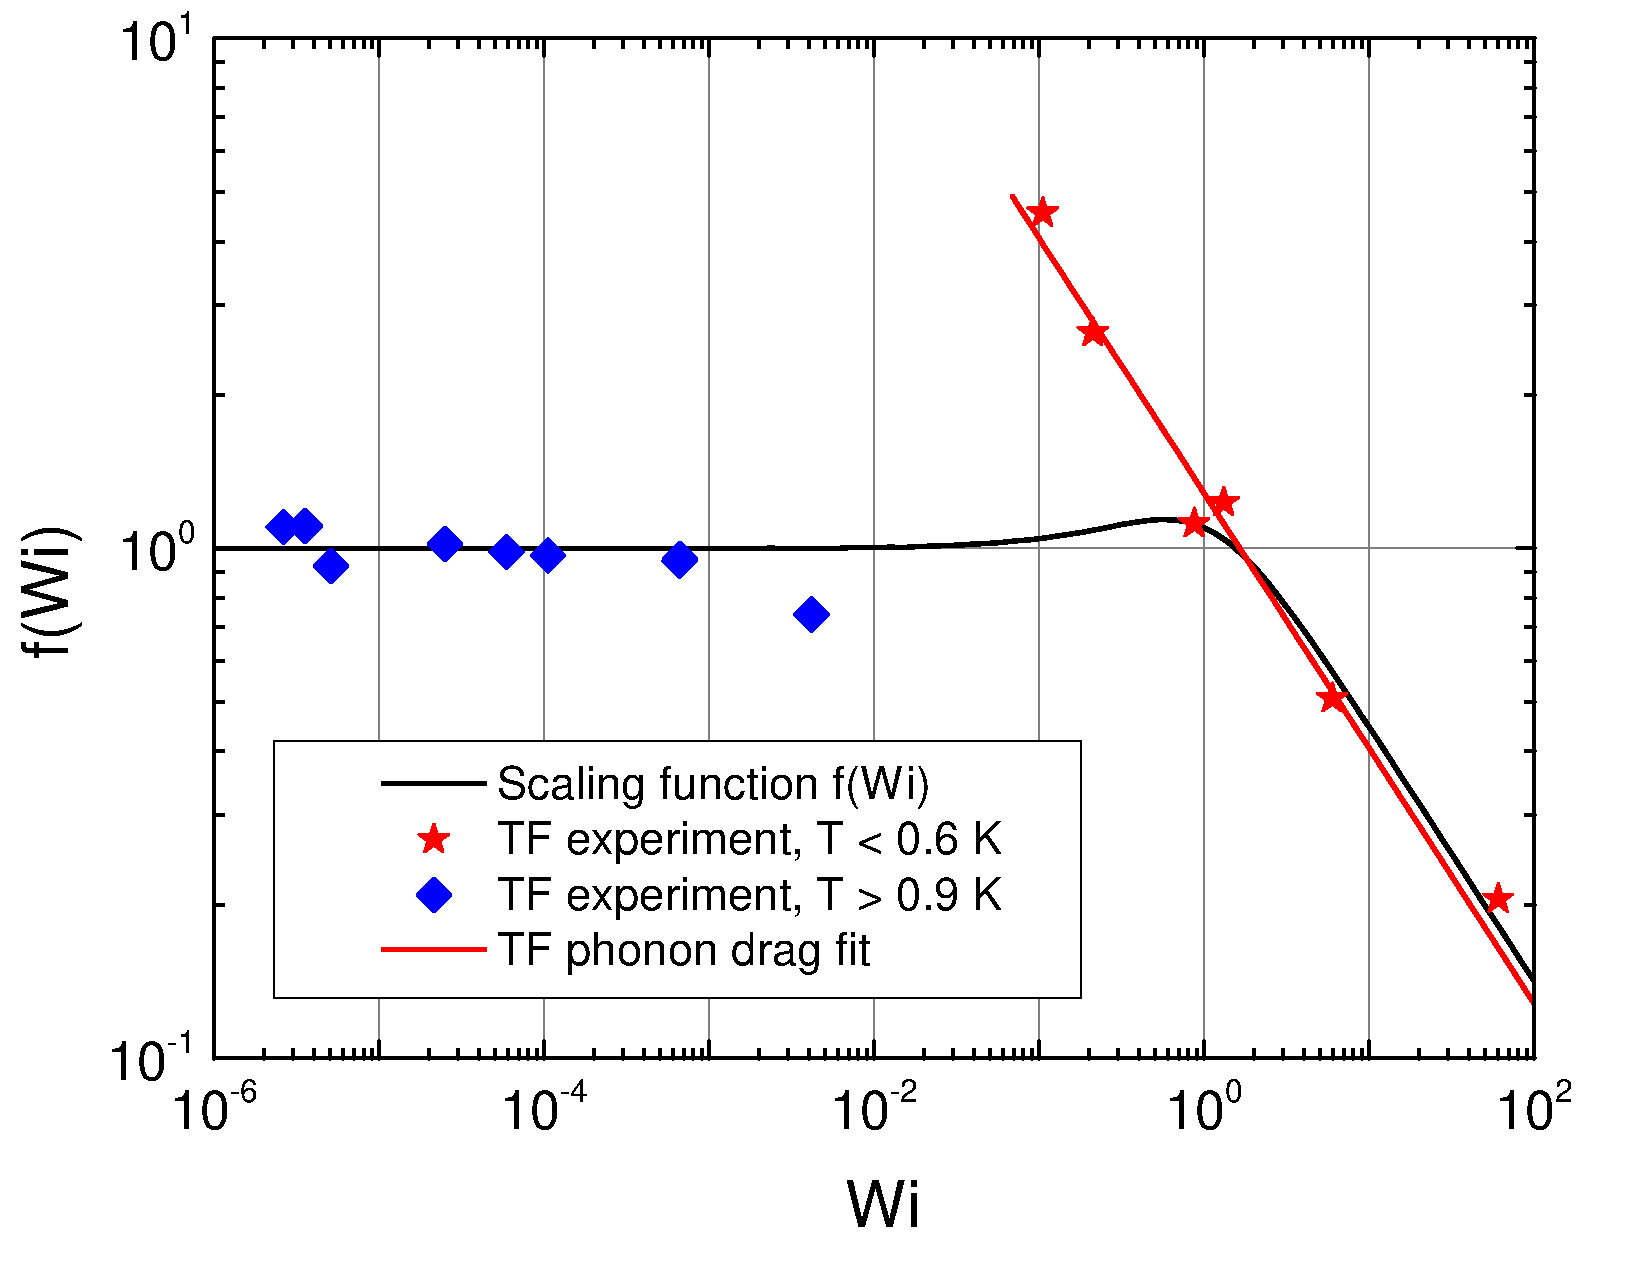
\includegraphics[width=0.7\textwidth]{graphics/results/ballistic_regime}
	\caption{Plot of scaling function $f(\text{Wi})$ as proposed in (\ref{scaling_function}) compared with the experimental results of tuning fork in both low and ultra-low temperatures.\\
	\underline{Black line:} fit of the scaling function, \underline{Red line:} fit to the phonon drag \cite{universal_scaling} , \underline{Blue squares:} experimental data collected from mentioned experiments, \underline{Red stars:} experimental data collected from ultra-low temperature range. In all experiments we used the same tuning fork on both oscillation modes.}
	\label{ballistic}
\end{figure}

Both asymptotics for $\text{Wi} \rightarrow 0$ and $\text{Wi} \rightarrow \infty$ are identical in the means of quasi-classical description of the excitation gas.
The mean free paths (or relaxation times) therefore can be calculated quantum-mechanically.\\
The derived behaviour of scaling function ($f(\text{Wi}) \sim 1$ for $\text{Wi} \ll 1$ and $f(\text{Wi}) \propto 1/\sqrt{\text{Wi}}$ for $\text{Wi} \gg 1$) reflects the experimental data, except for the transitional area $\text{Wi} \sim 0.1 $, where emerged a bigger peak than expected.\\
However, according to \textbf{Figure \ref{Kn-Wi}}, this is the range where the fluid have already reached the ballistic regime ($\text{Kn} \sim 1$) earlier than the non-Newtonian one ($\text{Wi} \sim 1$).
Hence, the assumptions for the scaling function derivation (that both $\text{Kn, Wi} \sim 1$) are no more valid and thus our prediction $f(\text{Wi}) \propto 1$ for the problematic area $\text{Wi} \sim 0.1$ does not hold.\\
In this case, the apparent scaling $f(\text{Wi}) \propto 1/\sqrt{\text{Wi}}$ simply means a frequency-independent drag force, as is expected for the ballistic regime.

\section{Flow phase diagram}

The last plot we show in \textbf{Experimental results} is the \textit{flow phase diagram}, summarizing the achieved hydrodynamical states by the oscillating tuning fork at various temperatures and modes. In \textbf{Figure (\ref{fork-flow_phase})} we also mark the estimated areas ("CT" for classical turbulence and "QT" for quantum turbulence), where the transitions to non-linear regimes emerge, separately for the normal and superfluid component.

\begin{figure}[h]
	\centering
	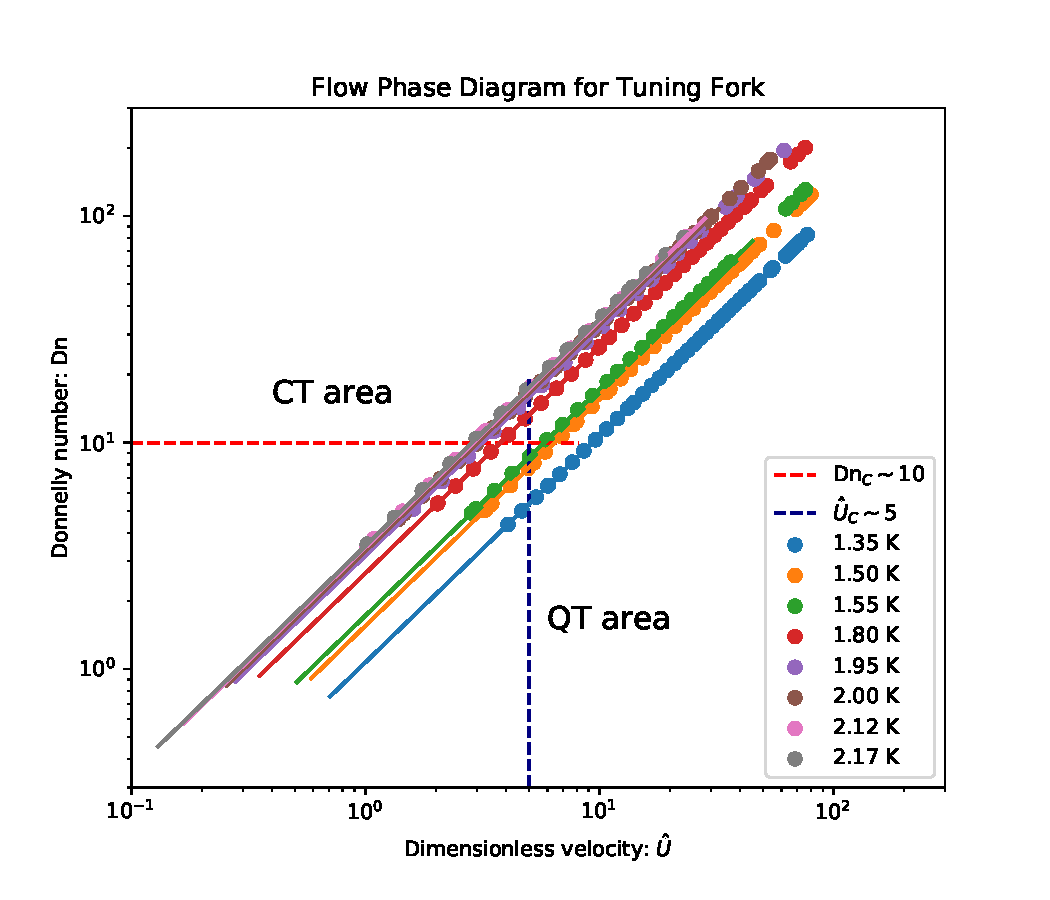
\includegraphics[width=0.8\textwidth]{graphics/results/fork-phase}
	\caption{Plot of Donnelly numbers against dimensionless velocities for both fork's oscillation modes. \underline{Full lines} fit the overtone mode data and \underline{dashed lines} the estimated areas of transition from laminar/potential regimes to the non-linear ones, both for normal and superfluid components.}
	\label{fork-flow_phase}
\end{figure}

It is worth to note that the \textit{CT area} and \textit{QT area} are not so sharp as it may seem from the graph. First of all, the most of the graph is covered by \textit{mixed turbulence} area since we already hinted that QT probably directly triggers CT.\\
Also, there could not be any more data above the $T=2.17\unit{K}$ curve since it is the natural limitation for the warmest Helium-II system.

\chapter{Simulations}

This part of Thesis serves as a general description of the \texttt{PyVort} codebase, a new platform to simulate quantum vortices. The code is written in well commented \texttt{Python 3}, arranged in a modular structure. The primary aim of this chapter is to highlight which modules are involved and how they work.
On \href{https://github.com/KuboBahyl/superfluid}{GitHub}, one can find a table of the parameters (user's options) which can be set in the \texttt{config.py} file to run the simulation.

At present, we use infinite boundary conditions. Therefore, only closed-loop vortices can be realized in simulation. However, the codebase is flexible and supports the potential implementation of unclosed loops.

\section{Vortex filament model}

The \texttt{PyVort} code is based on vortex filament (VF) model, a technique pioneerd by Schwarz \cite{schwarz} in the early 1980s. Superfluid vortex filament is represented by a series of mesh points (segments) distributed along the centerline of the filament (\textbf{Figure \ref{example_ring}}). The motion of the whole VF is summed up by the motion of each mesh point.

\begin{figure}[h]
	\centering
	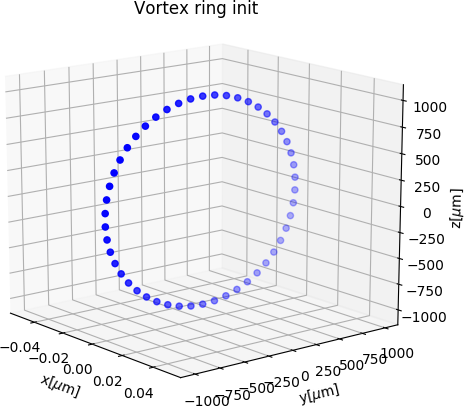
\includegraphics[width=0.5\textwidth]{graphics/simul/ring_init_crop}
	\caption{Visualisation of vortex ring segments right
after their initialisation.}
	\label{example_ring}
\end{figure}

As introduced in \textbf{Theoretical Background} chapter, we define the VF more precisely as a three dimensional curve $\vec{s}(\xi, t)$, where $\xi$ represents an arc-lengths and $t$ the time.
Each segment, indexed as $(i)$ ($i$ is increasing as we move along the VF) is localised by its assigned coordinates $\vec{s}_i$ and direct neighbours indices: \textit{previous} $(i-1)$ and \textit{next} $(i+1)$.\\
This leads to a data structure called \textit{directed digraph}, which we found as an useful array structure for vortex segments and thus was implemented.

Next we define the tangent vector $\vec{s}^{\prime}$, then normal vector $\vec{s}^{\prime\prime}$, and the binormal vector $\vec{s}^{\prime} \times \vec{s}^{\prime\prime}$, as depicted in \textbf{Figure \ref{filament}}, by taking numerical derivatives.
Note $\vec{s}^{\prime} = \text{d}\vec{s} / \text{d}\xi$ and $\vec{s}^{\prime\prime} = \text{d}\vec{s^{\prime}} / \text{d}\xi$.
Numerical derivatives are achieved using \textit{Finite Differences} method, as introduced in next subsection.


\subsection*{Finite differences}

In order to properly calculate the numerical derivatives $\vec{s}^{\prime}$ and $\vec{s}^{\prime\prime}$, belonging to the directed 3D curve, we need to use a sophisticated numerical method.
At a particular segment $(i)$ with position $\vec{s}_i$ , we define the distance to the next point $\vec{s}_{i+1}$ as $l_{i} = \vert \vec{s}_{i+1} - \vec{s}_i \vert$ and the distance to the previous point $\vec{s}_{i-1}$ as $l_{i-1} = \vert \vec{s}_i - \vec{s}_{i-1} \vert$ (\textbf{Figure \ref{FD}}).

\begin{figure}[h]
	\centering
	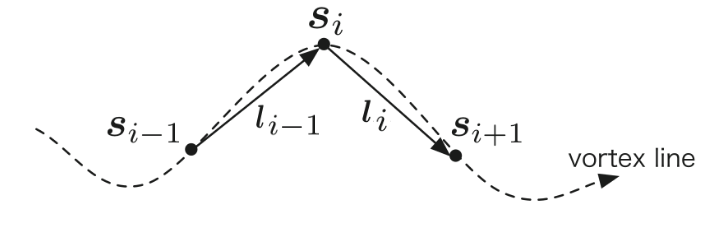
\includegraphics[width=0.8\textwidth]{graphics/simul/finite-diff}
	\caption{Depiction of $i$-th segment vector and its corresponding lengths. Source: \cite{tsubota}}
	\label{FD}
\end{figure}

For accuracy, we approximate all the spatial derivatives $\vec{s}_i^{\prime}$, $\vec{s}_i^{\prime\prime}$ by a
fourth-order finite difference method (FD), which can also account for the varying distances along the vortex filament. With this, the first and second derivatives can be obtained based on coordinates of 2 closest neigbours (on each side).

Using FD theorem, we can construct the approximations by taking the Taylor's series expansions. We can then write:

\begin{equation}
\frac{\text{d}^n\vec{s}_i}{\text{d}\xi^n} \approx
A_i\vec{s}_{i-2} +
B_i\vec{s}_{i-1} +
C_i\vec{s}_{i} +
D_i\vec{s}_{i+1} +
E_i\vec{s}_{i+2}
\hspace{1cm}
\text{for} \,n\in\{1,2\}
\label{FDcoeffs}
\end{equation}

Calculation of coefficients $A, B, C, D, E$ can be done using analytical solution of \textit{Vandermonde matrix} invertion. This invertion can be done also numerically, which is a more scalable way of implementation, however, this method often meets with problems when the Vandermonde matrix becomes singular.
In code, there is implemented both the analytical solution (closed form) and the solution by inverting the Vandermonde matrix. The closed form works for exactly our form of approximation (\ref{FDcoeffs}) and is more described in \cite{FDclosed}, whereas the numerical method works generally for any approximation level.

\subsection*{Biot-Savart discretisation}

We denote the dynamic external sources of velocity fields (which can be set in \texttt{config.py}) as $\vec{v}_{n,ext}(\vec{r}, t)$ and $\vec{v}_{s,ext} (\vec{r}, t)$. The equation of motion for a given segment is then given directly by Schwarz's equation(\ref{schwarz}):

\begin{equation}
\frac{\text{d}\vec{s}_i}{\text{d}t} =
\vec{v}_{s,ext} + \vec{v}_{\text{ind}}^{(i)} + \vec{v}_{\text{drive}}^{(i)}
\end{equation}

The first difficulty in the VF model comes from the calculation of term $\vec{v}_{\text{ind}}$. As we shown previously in (\ref{lia+biot}), this advection term can be split into the LIA part and a Biot-Savart integral:

\begin{align}
\vec{v}_{\text{ind}}^{(i)} =
\vec{v}_{\text{LIA}}^{(i)} + \vec{v}_{\text{BIOT}}^{(i)} =&
\frac{\varkappa}{4\pi} (\vec{s}^{\prime}_i \times \vec{s}^{\prime \prime}_i)
\ln{\Bigg(\frac{2\sqrt{l_{i-1} l_i}}{a}\Bigg)}
\label{LIA}
\\
+& \frac{\varkappa}{4\pi} \int_{\mathcal{L}^{\prime}} \frac{(\vec{r^{\prime}} - \vec{s}_i) \times \text{d}\vec{r^{\prime}}}{\vert \vec{r^{\prime}} - \vec{s}_i \vert^3}\,,
\label{BIOT}
\end{align}

where $l_{i-1}$ and $l_i$ are the arc lengths of the curve between
points $\vec{s}_{i-1}$ and $\vec{s}_i$ and between $\vec{s}_i$ and $\vec{s}_{i+1}$ respectively, and $\mathcal{L}^{\prime}$ is the original vortex line without the two segment lines between $\vec{s}_{i-1}$ and $\vec{s}_{i+1}$.

Using the segment discretisation, the Biot-Savart integral can be rewritten \cite{samuels} into the sum of single-line contributions (\textbf{Figure \ref{element}}) between each $j$-th and $j+1$-th segment (except for the ones attached to the $i$-th point):

\begin{equation}
\vec{v}_{\text{BIOT}}^{(i)} \approx
\frac{\varkappa}{4\pi}
\sum_{j \notin \{i-1, i\}}
\frac{(R_j + R_{j+1}) (\vec{R}_j \times \vec{R}_{j+1})}{R_j R_{j+1} (R_j R_{j+1} + \vec{R}_j \dotprod \vec{R}_{j+1})}\,,
\end{equation}

where $\vec{R}_j = \vec{s}_j - \vec{s}_i$ and $\vec{R}_{j+1} = \vec{s}_{j+1} - \vec{s}_i$ are the relative vectors from the given point.

Note that, if one takes into account the Biot-Savart law for $N$ mesh points, the computational time is proportional to $\mathcal{O}(N^2)$, while, if one uses just the LIA term, it is only $\mathcal{O}(N)$. Numerical simulations based on Biot-Savart are therefore significantly more computationally expensive.

\begin{figure}[h]
	\centering
	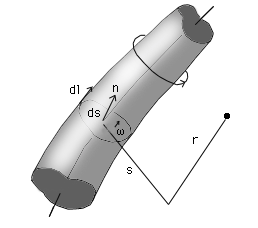
\includegraphics[width=0.4\textwidth]{graphics/simul/biot}
	\caption{An infinitesimal contribution of a $j$-th segment line between two points $\vec{s}_j$ and $\vec{s}_{j+1}$ at a given point $\vec{r}$. Source: \cite{element}}
	\label{element}
\end{figure}

One way to get around this difficulty is to update the LIA term. In this method we neglect completely the non-local Biot-Savart integral and keep just the local term. This is typically done with a minor adjustments within the log term:

\begin{equation}
\vec{v}_{\text{LIA}}^{*(i)} =
\frac{\varkappa}{4\pi} (\vec{s}^{\prime}_i \times \vec{s}^{\prime \prime}_i)
\ln{\Bigg(\frac{2 R_i}{a}\Bigg)}\,,
\label{LIAnew}
\end{equation}

where $R_i$ is a $i-th$ segment local length scale - may be taken \cite{barenghi} as a local curvature: $R_i = 1 / \vert \vec{s}^{\prime \prime}_i \vert$. Updated LIA approach (\ref{LIAnew}) is a very convenient approximation and works very well for calculating the motion of a single vortex ring.

\section{Implementation}

In code, a system consisting of flow sources and a single vortex ring object is represented using several \texttt{class} structures. These structures are updated after each time step. We will call them as a \textit{state} of the system and it is defined (and initialised) with following properties:

%\newpage

\subsection*{Environment class}

\begin{itemize}
	\item \underline{external normal component} - defines an external source of normal component flow
	\item \underline{external superfluid component} - defines an external source of superfluid component flow
\end{itemize}

\subsection*{Ring class}

This class is initialized only when the purpose of simulation is to collect physical and statistical data about vortex rings.

\begin{itemize}
	\item \underline{center} - an array of ring center coordinates
	\item \underline{radius} - current radius $R$ of the ring object
	\item \underline{direction} - a normal vector $\vec{\hat{n}}$ pointing in a direction toward which the ring is moving
	\item \underline{velocity} - measured velocity of the ring center $\vec{v}_{\text{ring}}$
\end{itemize}


\subsection*{Vortex class}

\begin{itemize}
	\item \underline{number of active segments} - number of active segments $N$ the vortex ring is composed of
	\item \underline{segments} - an array of all segments, each one with following attributes:
	\begin{itemize}
		\item \underline{activity} - a logical value whether a particular segment should be considered as a part of vortex object
		\item \underline{coordinates} - an array of segment coordinates $\vec{s}_i = [x_i,y_i,z_i]$
		\item \underline{previous/next neighbour} - array localisation indices of the \textit{previous} $(i-1)$ and the \textit{next} $(i+1)$ segment within the context of the directed vortex
		\item \underline{tangent/curvature} - a tangential and normal vectors $\vec{s}^{\prime}_i$ and $\vec{s}^{\prime\prime}_i$

		\item \underline{LIA velocity} - a self-induced velocity $\vec{v}_{\text{LIA}}^{(i)}$ driven by the local curvature. (\ref{LIA}) or (\ref{LIAnew})
		\item \underline{BIOT velocity} - a self-induced velocity driven by the farther segment lines of the vortex ring $\vec{v}_{\text{BIOT}}^{(i)}$ (\ref{BIOT})

		\item \underline{Drive velocity} - a velocity given by the mutual friction force $\vec{v}_{\text{drive}}^{(i)}$ (\ref{drive})
		\item \underline{Full velocity} - the sum of external sources $\vec{v}_{s,ext}$, LIA velocity $\vec{v}_{\text{LIA}}^{(i)}$, BIOT velocity $\vec{v}_{\text{BIOT}}^{(i)}$ and the drive velocity $\vec{v}_{\text{drive}}^{(i)}$, resulting in $\text{d}\vec{s}_i / \text{d}t$
	\end{itemize}
\end{itemize}

All functions that are manipulating with segments' attributes are implemented as Vortex class methods. Before each time step, all attributes have to be updated and tested. We used numerical methods already introduced in previous section and tests that are described in next section.

\subsection*{Initialisation}

The proper initialisation of the \textit{state} in the very beginning of simulation requires several physical inputs. This is done in following steps:
\begin{itemize}
	\item[0.] Symbolically, we expect as a \textit{0-th step} the environmental setup of the system - \textit{external sources, temperature, time-step,...}.

	\item[1.] If interested in quantized ring simulation, we expect several ring inputs from user: \textit{center, radius, direction} and \textit{resolution}.
	Resolution parameter is the initial desired distance $\delta$ between each two neigbouring segments. This set of 4 inputs makes an unambiguous ring object, ready for next updates.

	\item[2.] After creation, we initialise neigbour indices (to an $i$-th element in segment array will be assigned $i-1$ index as the \textit{previous} and $i+1$ index as the \textit{next} neighbour index)
	\item[3.] Next we calculate all $\vec{s}^{\prime}$ and $\vec{s}^{\prime\prime}$ using Finite differences method
	\item[4.] Final step is the calculation of all segment velocities using motion equations and their approximative forms.
\end{itemize}

After these four steps, we obtain a fully updated ring object that can be propagated in time.

\section{Time evolution}

After we defined and ran all the necessary calculations leading to the vortex ring's \textit{state} fulfillment, we can start to propagate it in time (visualised example in \textbf{Figure \ref{motion}}).

\begin{figure}[h]
	\centering
	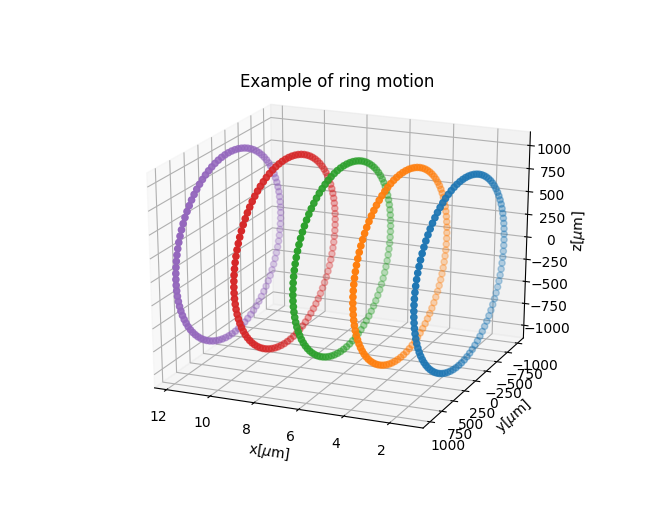
\includegraphics[width=0.8\textwidth]{graphics/simul/time-example}
	\caption{Example of a moving vortex ring}
	\label{motion}
\end{figure}

\subsection*{Time stepping}

Time evolution is based on an explicit iterative method: the fourth-order Runge-Kutta (RK4) scheme. When we consider the Schwarz's equation $\text{d}\vec{s}_i / \text{d}t \equiv \vec{v}_{\text{full}}^{(i)}$, the stepping algorithm is given as:

\begin{equation}
\vec{s}_{i}(t+\text{d}t) =
\vec{s}_{i}(t) +
\frac{\text{d}t}{6} (\vec{v}_1^{(i)} + 2\vec{v}_2^{(i)} + 2\vec{v}_3^{(i)} + \vec{v}_4^{(i)})\,,
\end{equation}

where $\text{d}t$ is the time step and the velocities $\vec{v}_1^{(i)}, \vec{v}_2^{(i)}, \vec{v}_3^{(i)}, \vec{v}_4^{(i)}$ are the induced velocites of partial steps:

\begin{align}
\vec{v}_1^{(i)} =& \vec{v}_{\text{full}}^{(i)}
(\vec{s}_i, t)\,,
\\
\vec{v}_2^{(i)} =& \vec{v}_{\text{full}}^{(i)}
(\vec{s}_i + \vec{v}_1^{(i)} \text{d}t / 2, t + \text{d}t / 2)\,,
\\
\vec{v}_3^{(i)} =& \vec{v}_{\text{full}}^{(i)}
(\vec{s}_i + \vec{v}_2^{(i)} \text{d}t / 2, t + \text{d}t / 2)\,,
\\
\vec{v}_4^{(i)} =& \vec{v}_{\text{full}}^{(i)}
(\vec{s}_i + \vec{v}_3^{(i)} \text{d}t, t + \text{d}t)
\end{align}

Lower-order schemes such as basic Euler method is also implemented in code, however, not recommended to use. More on this is discussed in Results part of thesis.

The time step $\text{d}t$ is adaptively changing so that the vortex ring cannot move faster than a $1\%$ of its size in a single step. As we will see later in Results, in case of vortex rings with changing radius, the time step $\text{d}t$ has to be iteratively changing after each break of the above rule:

\begin{equation}
\text{d}t \leftarrow \frac{0.01 R}{\vert \vec{v}_{\text{ring}} \vert}
\label{adaptive_dt}
\end{equation}

\section{Re-segmentation of vortex}

To obtain the most realistic simulation (to capture effects on any length scale), the natural tendency would be to set the resolution parameter $\delta$ as low as possible. However, the CPU time cost rises rapidly as the number of segments $N$ increases, so there is need to find the best trade-off.

As the distance between neighbouring segments is reduced/enlarged with time due to the physics and numerical inaccuracies, there is need to remove/add segments (\textit{re-segment}) in order to conserve the vortex resolution $\delta$. The closeness (in terms of arclength) of neighbouring segments is therefore measured after each simulation time-step.

We used the simplest re-segmenting criteria - keeping an approximately \textit{uniform distance} between the segments. To ensure this, two boundary conditions were implemented:

\begin{itemize}
	\item[1.] The segment $\vec{s}_{j+1}$ would be removed if:

	\begin{equation}
	\vert \vec{s}_{j+1} - \vec{s}_j \vert < \delta_{\text{min}}\,,
	\end{equation}

	where $\delta_{\text{min}}$ is the minimal distance between two segments. Also, the segment $\vec{s}_j$ would take place somewhere between $\vec{s}_{j-1}$ and $\vec{s}_{j+2}$ so that it will conserve the curvature of vortex. Such result can be obtained using any spline interpolation along nearest neighbours. We worked with 3D local spline using 4 points (in our context they would be $\vec{s}_{j-2}$, $\vec{s}_{j-1}$, $\vec{s}_{j+1}$, $\vec{s}_{j+2}$) and create another 11 interpolated knots.
	Consequently, the new position of $\vec{s}_j$ will be the position of the 6-th knot (the middle one).

	\item[2.] We add a new segment $\vec{s}_{\text{new}}$ between $\vec{s}_{j}$ and $\vec{s}_{j+1}$ if:

	\begin{equation}
	\vert \vec{s}_{j+1} - \vec{s}_j \vert > \delta_{\text{max}}\,,
	\end{equation}

	where $\delta_{\text{max}}$ is the maximal allowed distance between two segments.
\end{itemize}

This method keeps all the distances along the vortex roughly in the range $\delta \in \langle \delta_{\text{min}}, \delta_{\text{max}} \rangle$ and also keeps the geometrical properties.

\subsection*{Real-time tests}

After each time step is done, a few tests are performed, to ensure that vortex itself is behaving according to our expectations. The tests are following:

\begin{itemize}
	\item \underline{Length test} - This test calculates the segmented vortex circumference as $l = \sum_j \vert \vec{s}_j - \vec{s}_{j+1} \vert$ and compare it with the theoretical one $2\pi R$, where radius $R$ has to be measured as well. If the deviation from the theoretical value is too high $>1\%$, the segments are noisy and the process is killed. In case of deviation below $<-1\%$, there are clearly too few segments and resegmentation process is called.

	\item \underline{Segmentation test} - Here we check the value $l_j = \vert \vec{s}_j - \vec{s}_{j+1} \vert$ for each $j$ and ask whether $l_j \in \langle \delta_{\text{min}}, \delta_{\text{max}} \rangle$. If not, resegmentation process is called.

	\item \underline{Smallness test} - If the vortex ring radius would decrease below $R < \delta_{\text{min}}$, the ring is deleted from the simulation.
\end{itemize}

\section{Future implementations}

To make \texttt{Pyvort} a full-fledged quantum vortex simulation, there should be implemented following improvements:

\subsection*{Complexity speedup}

Recent numerical research presented \cite{tree_alg} a new numerical method to compute the evolution of vortex filament. The method is based on an N-body cosmological simulation by Barnes and Hut \cite{barnes}, a \textit{tree algorithm} which considerably speeds up the calculation of Biot-Savart integrals - computational cost scales as $\mathcal{O}(N \log(N))$ rather than $N^2$. Properties of the tree method were tested for a variety of vortex configurations, ranging from simple vortex rings to a counterflow vortex tangle and compared with the LIA approach and the exact Biot-Savart's law.

Implementation of such algorithm is not easy, but definitely worth due to the gain in efficiency.


\subsection*{Re-connection process}

If any lines of two vortices (or even the single one) become very close,
the filaments can reconnect, changing the topology of the system.
Many researchers experimentally reported this is happening and also found analogies with vortex dynamics in the Navier–Stokes equation.

\begin{figure}[h]
	\centering
	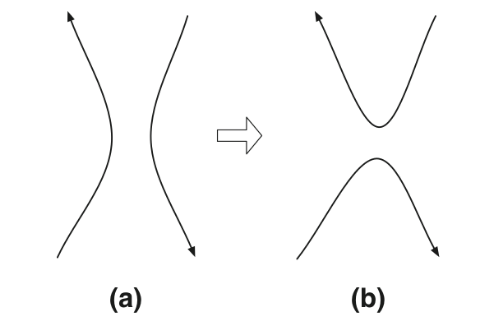
\includegraphics[width=0.6\textwidth]{graphics/simul/reconnection}
	\caption{Reconnection of quantized vortices. \textbf{(a)} Two vortices before reconnection, about to contact each other. \textbf{(b)} The new vortices after reconnection.}
\end{figure}

The VF model itself cannot describe the reconnection process because the vortex core structure is neglected. Hence, some artificial procedures must be introduced to simulate such process. For instance, when two vortices approach within a critical distance $\delta_{\text{min}}$, we will artificially reconnect the vortices.

The main criteria for reconnection is that the total length (this is corresponding with energy) will decrease. Self-reconnections (e.g. caused by a twist of vortex) would be treated in the same way. Since recconection involves only antiparallel vortices, one has to check using the inner product whether two vortices could physically reconnect or not.

\subsection*{High-order tests}

Once the code of interacting vortex filaments is developed, the data analysis needs to be improved. The simplest measurable quantity is the total lenght of all vortex lines. In a finite volume this would be $L = (1/V) \int \text{d}\xi$ for the vortex length per unit volume.

Of course, one may define more complicated metrics, measuring the isotropy of the vortex tangle. One of them is the length of line projected along a given vector $\vec{\hat{r}}$, given as:

\begin{equation}
J(\vec{\hat{r}}) = \frac{1}{VL} \int_{\mathcal{L}} \sqrt{1 - (\vec{s}^{\prime}(\xi) \dotprod \vec{\hat{r}})^2} \text{d}\xi
\end{equation}

\newpage

\chapter{Simulation Results}
% \begin{itemize}
% 	\item does num segments affect the initial ring velocity?
% 	\item does energy (and velocity) changes if Quantum=False?
% 	\item for a given R and euler method, what is the life of stability for various num segments
% 	\item when is it good to resegment?
% 	\item which config leads to the death of the ring for various R
% 	\item measure death time and distance for various R
%
% \end{itemize}
%
% \section{Vortex ring}
% \begin{itemize}
% 	\item compare rings with various radii
% 	\item theoretical vs simulation velocity / range
% 	\item stability tests
% 	\item initialisation
% 	\item movement, decreasing radius
% 	\item comparison with theory
% \end{itemize}

In this chapter, we analyse the functionality of new codebase. We made several tests on energy conservation, precision of numerical methods and stability, to ensure that simulation is reliable and stable for further development.

All presented measurements and optimisations were conducted in order to recommend the best simulation parameters for future investigations, which is ensured by the correct setup of the \texttt{config} file. We performed tests with physical motivation and also tests focused on precision and stability. With presented findings, the reliability and stability of any further large-scale simulation should be ensured.

\newpage

%%%%%%%%%%%%%%%%%%%%%%%%%%%%%%%%%%%%%%%%%%%%%%%%%%%%%%%%%%%%%%%%%%%%%%%%%%%%%%%%%%%%%%%%%%%%%%%%%%%%%%%%%%%%%%%%%%%%%%%%%%%%%%%%%%%%%%%%%%%%%%%%%%%%%%%%%%%%

\subsection{Zero-temperature test}

In case of zero temperature $T=0\unit{K}$, the \textit{normal component} in superfluid He-II is not present anymore and therefore also no mutual friction. Even the mutual friction is not the only present dissipation process (we neglect phonon emissions), we expect for out numerical model to conserve the velocity and energy of the vortex ring.

We plotted in \textbf{Figure \ref{Tzero}} the ring velocity $\vert \vec{v}_{\text{ring}} \vert $ and energy $E_{\text{ring}}$ evolving in time, for the case of temperature $T=0$ (pure superfluid, no normal component) and $T=1.5\unit{K}$ (considerable ratio of present normal and superfluid component $\rho_s / \rho_n \approx 8$).\\
We tested the mutual friction effect during 1000 time-steps (refered to as \textit{epochs}) with adapting timestep $\text{d}t$ according to (\ref{adaptive_dt}).

\begin{figure}[h]
	\centering
	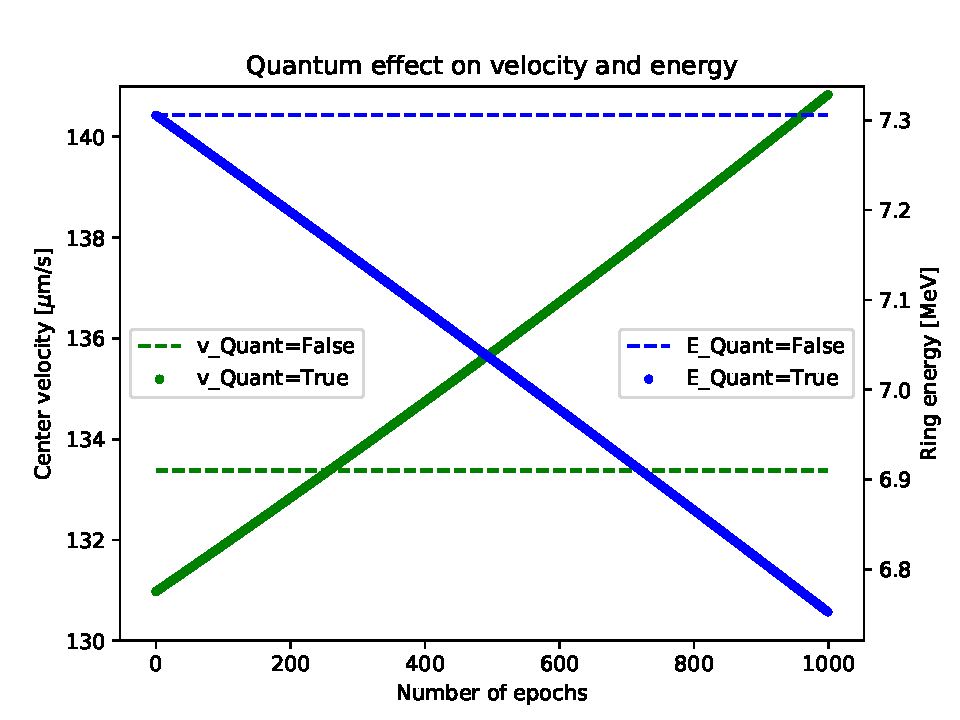
\includegraphics[width=0.8\textwidth]{graphics/results/Tzero}
	\caption{Evolution of ring velocity and energy in time. \underline{Blue lines} - measured velocity data, \underline{Black lines} - measured energy data,
	\underline{Dashed lines} - the constant behaviour for temperature $T=0\unit{K}$, \underline{Full lines} - the dissipative process for temperature $T=1.5\text{K}$.\\
	On \texttt{x} axis, we plot the number of elapsed epochs (time steps) and on \texttt{y} axis the velocity of the ring center $\vert \vec{v}_{\text{ring}} \vert $ and ring energy $E_{\text{ring}}$.}
	\label{Tzero}
\end{figure}

As we see, at $T=0\unit{K}$ the velocity and energy is conserved even after 1000 epochs of simulation due to missing dissipation process (mutual friction). In case of $T=1.5\unit{K}$, energy is descreasing as expected, whereas the velocity is increasing. This increase is physically well-explained by the fact that the radius is decreasing with time due to the non-dissipative term of mutual friction. Also, it can be seen directly from the theoretical formula (\ref{ring-velocity}).

%%%%%%%%%%%%%%%%%%%%%%%%%%%%%%%%%%%%%%%%%%%%%%%%%%%%%%%%%%%%%%%%%%%%%%%%%%%%%%

\subsection{Velocity precision test}

Our first velocity test compares the various approaches how can the ring velocity $\vert \vec{v}_{\text{ring}} \vert $ be calculated. Here, we compare four approaches, recognizing their theoretical motivation, computational complexity and precision:
\begin{itemize}
	\item LIA (\ref{LIA}): motivated \cite{barenghi}, computationally cheap, not precise
	\item LIA + BIOT (\ref{LIA} + \ref{BIOT}): motivated \cite{barenghi}, but computationally expensive
	\item updated LIA (\ref{LIAnew}): not well motivated \cite{samuels}, but computationally cheap and precise
	\item Theoretical (\ref{ring-velocity}): well motivated \cite{roberts} and most precise
\end{itemize}

\begin{figure}[h]
	\centering
	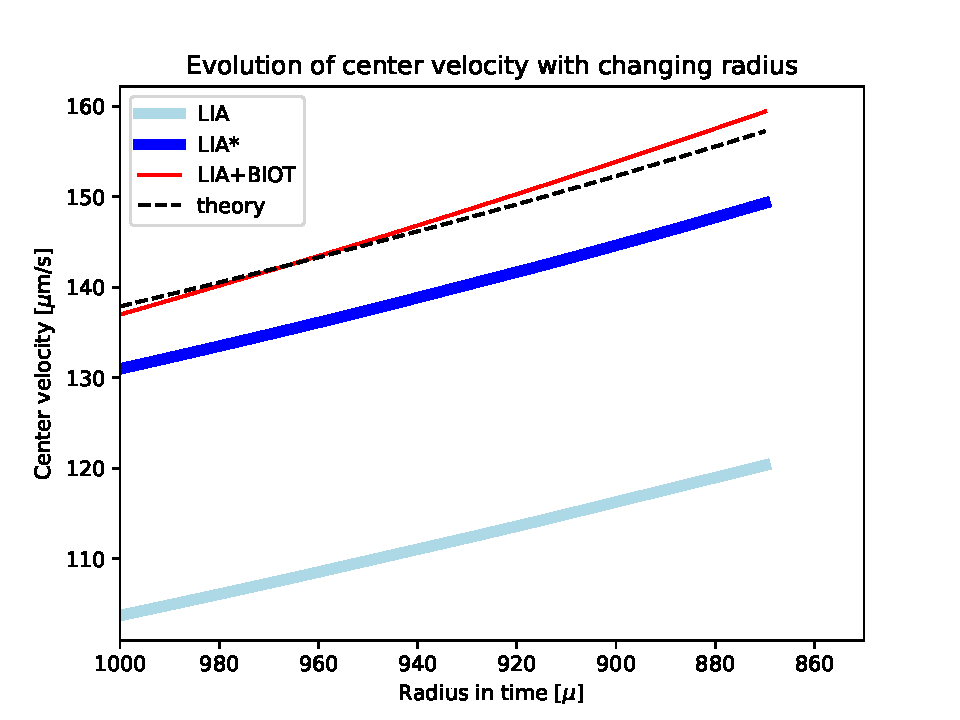
\includegraphics[width=0.8\textwidth]{graphics/results/vels_radius}
	\caption{Comparison of all implemented velocity approaches (\underline{full lines}) with the theoretical one (\underline{black dashed line}) according to (\ref{ring-velocity}), with decreasing radius in time.\\
	Velocity values $\vert \vec{v}_{\text{ring}} \vert$ on \texttt{y} axis are computed always using the measured decreasing radius value (\texttt{x} axis)}
	\label{vels-radius}
\end{figure}

The theoretical values of ring velocity from (\ref{ring-velocity}) are taken as a baseline that other velocity calculations are compared with.
All velocites were measured and evolved over a few thousands epochs (time steps), during which the radius was dissipatively decreasing, as is plotted in \textbf{Figure \ref{vels-radius}}.

We see that the theoretically most precise (LIA + BIOT) approach grows a bit faster than it should according to theory. This inconsistence is caused by too big resolution parameter, which was set at $\delta \approx 70 \mu \unit{m}$\\
Therefore, for all further measurements we used the updated LIA velocity (LIA*) approach due to its time-scale consistency and computational speed.

%%%%%%%%%%%%%%%%%%%%%%%%%%%%%%%%%%%%%%%%%%%%%%%%%%%%%%%%%%%%%%%%%%%%%%%%%%%%%%

\subsection{Velocity convergence test}

Next, we investigated the magnitude of the ring velocity $\vert \vec{v}_{\text{ring}} \vert$ for various resolutions $\delta \in \langle 50, 200 \rangle \mu\text{m}$, immediately after initialisation and then after 100 epochs. Ring radius was always set at $R=1000\mu\text{m}$ (this is usual working radius \cite{tsubota} \cite{FDclosed}), so the number of discretisation points along the vortex was given by $R$ and $\delta$ as $N \approx 2\pi R/ \delta \in \langle 30,120 \rangle$.

\begin{figure}[h]
	\centering
	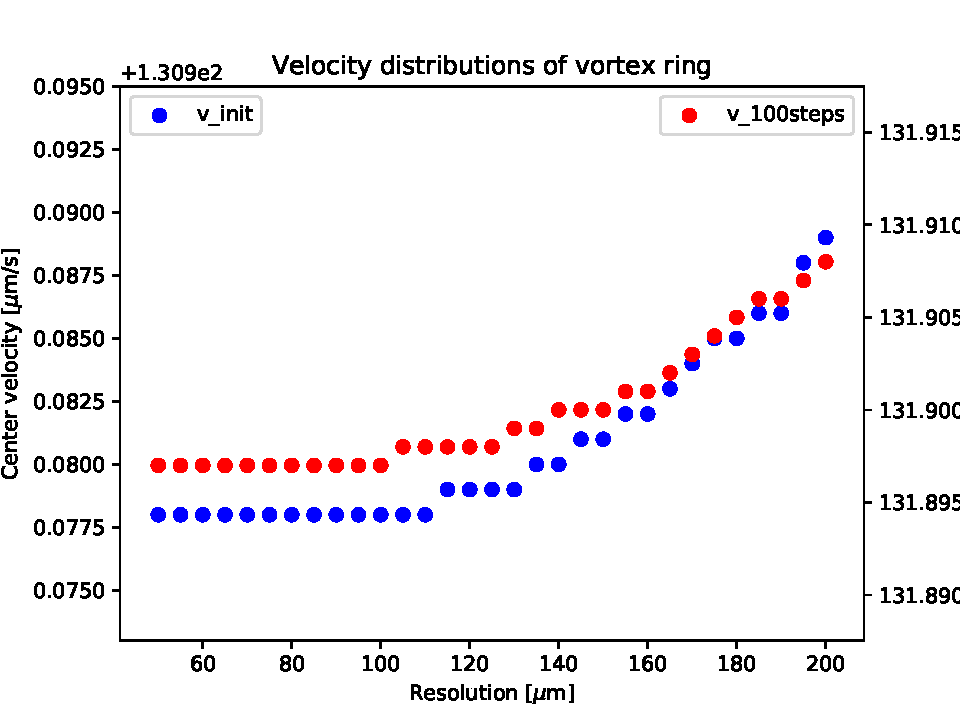
\includegraphics[width=0.8\textwidth]{graphics/results/vels_convergence}
	\caption{The distribution of ring velocity values $\vert \vec{v}_{\text{ring}} \vert$ for a range of resolution paramters $\delta$ in two situations. \underline{Blue dots} - Velocity values immediately after initialisation, \underline{Red dots} - velcotiy values after 100 time-steps.\\
	On \texttt{x} axis, we plot the resolutions $\delta$ of vortex segments and on \texttt{y} axis the ring velocity $\vert \vec{v}_{\text{ring}} \vert$.}
	\label{vels-converg}
\end{figure}

We see in \textbf{Figure \ref{vels-converg}} the expected convergent behaviour of both measured velocities in the range of good resolutions (small values of $\delta$). It seems that below $ \delta < 100 \mu\text{m}$  (corresponding to $\approx 60$ segments along the ring of radius $R=1000 \mu \unit{m}$) the velocites are converged, which provides the upper boundary for a \textit{good-chosen} resolution.

Even if it is intuitive that good resolutions (small $\delta$-s) lead to more precise velocities, the high number of vortex segments $N \propto 1/\delta$ worsens the stability of simulation in time. The reason behind this effect is the assumption of \textit{RK4} stepping method that functions, which \textit{RK4} is approximating, are smooth. With higher number of segments, there is higher chance for the ring to be non-smooth, which leads to exponential errors in \textit{RK4} algorithm.

Therefore, we propose also a lower boundary for  $\delta$, ensuring the stability, in a following test in next subsection.

%%%%%%%%%%%%%%%%%%%%%%%%%%%%%%%%%%%%%%%%%%%%%%%%%%%%%%%%%%%%%%%%%%%%%%%%%%%%%%

\subsection{Stability test}

Stability of simulation in time was measured for a range of resolutions $\delta \in \langle 10, 100 \rangle \mu\text{m}$ and three values of vortex radius $R \in \{500, 1000, 2000\} \mu\text{m}$ using \textit{Euler} and \textit{RK4} stepping method. In all cases, the stability is measured by the maximal number of elapsed epochs, till the simulation was forced to stop.
This enforcement was determined by the violation of length condition, as was described in \textbf{Real-time tests} subsection- the real vortex circumference $l = \sum_j \vert \vec{s}_j - \vec{s}_{j+1} \vert$ cannot deviate more than $1\%$ from the geometrical value $2\pi R$, where $R$ is the measured radius in current state.

\begin{figure}[h]
	\centering
	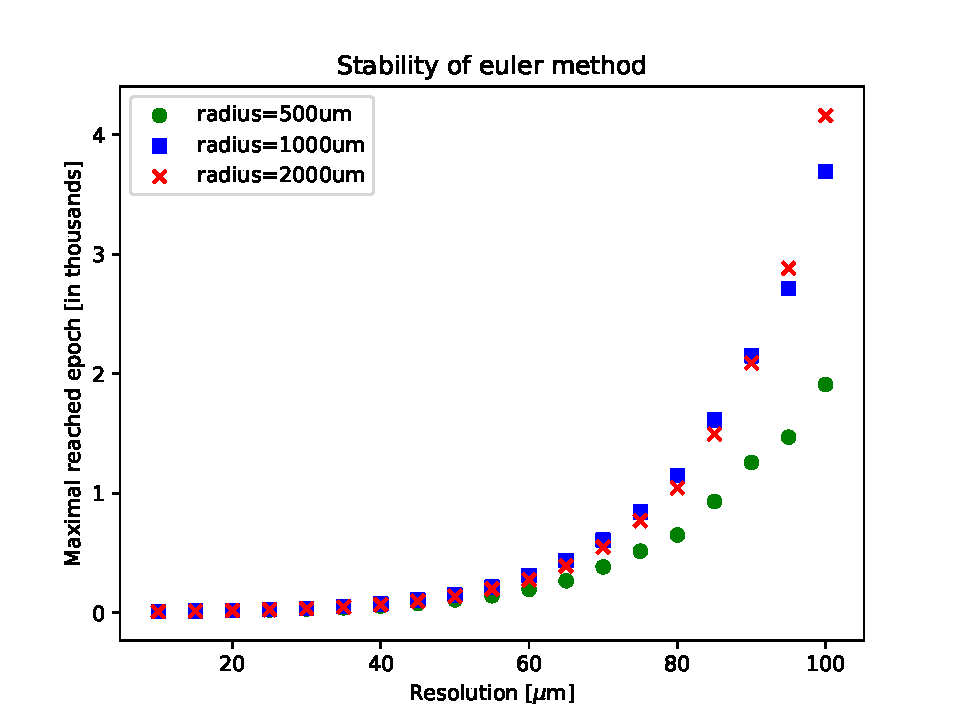
\includegraphics[width=0.8\textwidth]{graphics/results/stability-euler}
	\caption{Plot of maximal elapsed epoch (time step) of simulation with a given resolution $\delta$, radius $R$ and \textit{Euler} stepping method, till the simulation was forced to stop by violating the length condition.}
	\label{stab-euler}
\end{figure}


From the plot in \textbf{Figure \ref{stab-euler}}, the \textit{Euler} method seems to be unstable for all resolutions $\delta \in \langle 10, 100 \rangle \mu\text{m}$. Such behaviour was expected and simulated only as an example of inappropriately chosen stepping method.

The next experiment was conducted with \textit{RK4} method, a much more stable method comparing with the \textit{Euler} one, but also suffering from strong assumptions (smoothness of evoluting function). After the same experiment with changed time-step method was performed, we measured a stronger stability:

\begin{figure}[h]
	\centering
	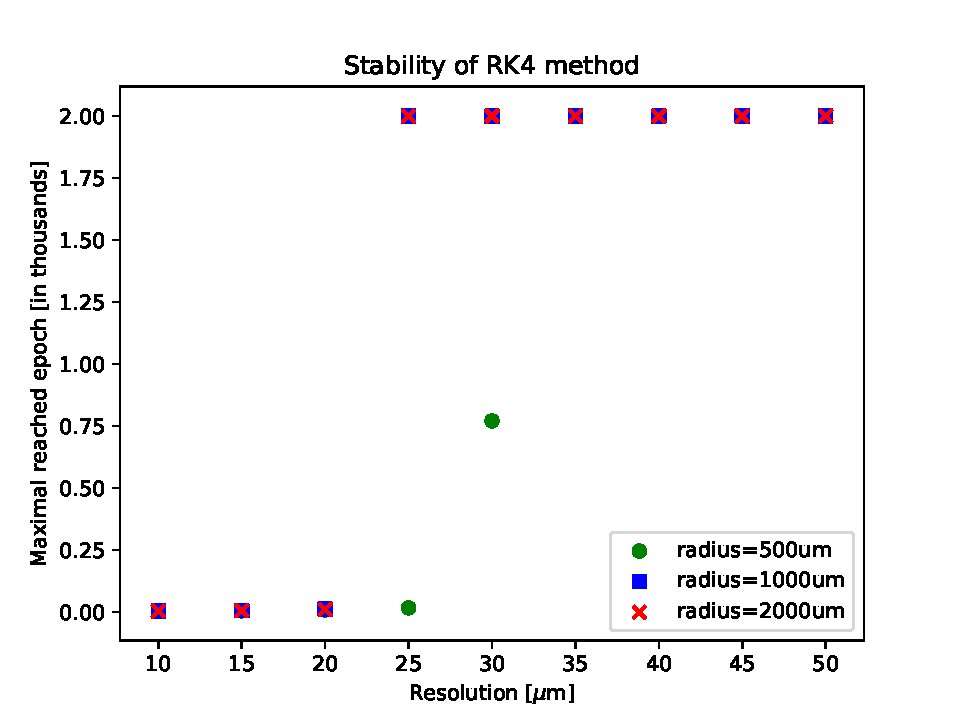
\includegraphics[width=0.8\textwidth]{graphics/results/stability-RK4}
	\caption{Plot of maximal elapsed epoch (time step) of simulation with a given resolution $\delta$, radius $R$ and \textit{RK4} stepping method, till the simulation was forced to stop by violating the length condition. A threshold is set on $2000$ epochs.}
	\label{stab-rk4}
\end{figure}

The plot in \textbf{Figure \ref{stab-rk4}} suggests the minimal resolution to be at least $\delta >30\mu\text{m}$. This boundary estimate is still quite conservative, since the radius of vortex is decreasing in time and resegmentation processes will happen.
Resegmantation process significantly contributes to the stability of simulation since the deletion of some segments behaves as a \textit{smoothing effect} which supports the \textit{RK4} method to be stable.

\newpage

\chapter{Conclusions}

In this chapter we summarize the foundings of analysed experiments from \textbf{Experimental Results} chapter and of numericalal experiments ftom the \textbf{Simulation} chapter.

\section{Experimental conclusions}

We investigated systematic high-Stokes flows of Helium-II at a range of temperatures $T \in \langle 1.35 \unit{K}, 2.17 \unit{K} \rangle$ generated by several types of oscillators - \textit{vibrating wire, torsionally oscillating disc and tuning
fork}. All of them were kept in high-frequency limit to ensure the Stokes number to be St$\gg 1$.

Within the area of \underline{low peak velocities}, we showed the normal component behaving laminar ($C_D^{\, n} \propto \text{Dn}^{-1}$) and superfluid component remaining potential (or stationary in case of torsional disc).\\
When we consider only a \underline{negligible amount} of remnant quantized vortices attached to the oscillator body, the normal and superfluid components have independent velocity fields, so the measured drags can be analysed separately as well. In this limit we treat the normal component as a classical viscous fluid, resulting naturally in inverse scaling of measured normal drag coefficient with the Donnelly number: $C_D^{\, n} \propto \text{Dn}^{-1}$.\\
Assuming that superfluid component doesn't contribute to the drag, the universal scaling holds until a critical velocity $U_C$ for a given oscillator geometry is reached. Or, generalising it for all oscillator modes $\{\omega_i\}$, until a \underline{critical dimensionless velocity} $\hat{U}_C = U_{C_i} / \sqrt{\varkappa \omega_i}$ is reached.

In general, we distinguish between \underline{4 types} of hydrodynamical states of Helium-II. We label the instabilities formed due to normal component as "CT" (classical turbulence) and due to superfluid component as "QT" (quantum turbulence):

\begin{itemize}
	\item \underline{No CT nor QT present:} laminar regime as described above, working universal scaling on normal component, superfluid component is potential or not moving at all, observed with all used oscillators ($\text{Dn} \lesssim 1$ for vibrating wire, $\text{Dn} \lesssim 5$ for oscillating disc and $\text{Dn} \lesssim 10$ for both oscillation modes of tuning fork).

	\item \underline{CT present without QT:} normal component expected to start exhibiting a classical non-linear behaviour after reaching critical value of Donnelly number $\text{Dn}_C$ (thus universal scaling still holds), superfluid component expected to remain potential or motionless, observed only with tuning fork at both oscillation modes for temperatures higher than $T > 1.6\unit{K}$ with low Donnelly numbers between $10 \lesssim \text{Dn} \lesssim 100$.

	\item \underline{QT present without CT:} occurs if critical velocity $U_C$ given by Donnelly-Glaberson instability (reconnection of remnant vortices) is achieved sooner than the critical Donnelly number $\text{Dn}_C$. Generally it is hard to prove whether such situation occured since the CT is usually triggerred almost immediately due to thw mutual friction.

	\item \underline{Both CT and QT present:} both normal and superfluid components are expected to contribute to the drag, occuring when both critical velocity $U_C$ and Donnelly number $\text{Dn}_C$ are reached (or triggerred), observed with all used oscillators.
\end{itemize}

To summarize, Donnelly-Glaberson instability (launching QT) occurs upon reaching a \textbf{critical dimensionless velocity} $\hat{U}_C$, while the instability in the normal component is governed  upon reaching a \textbf{critical Donnelly number} $\text{Dn}_C$. All of the phase states were observed during experiments on oscillating bodies as described in previous chapters.

We summarize all oscillators, once again in the \textit{flow phase diagram} in \textbf{Figure \ref{flow_phase_diagram}}:

\begin{figure}[h]
	\centering
	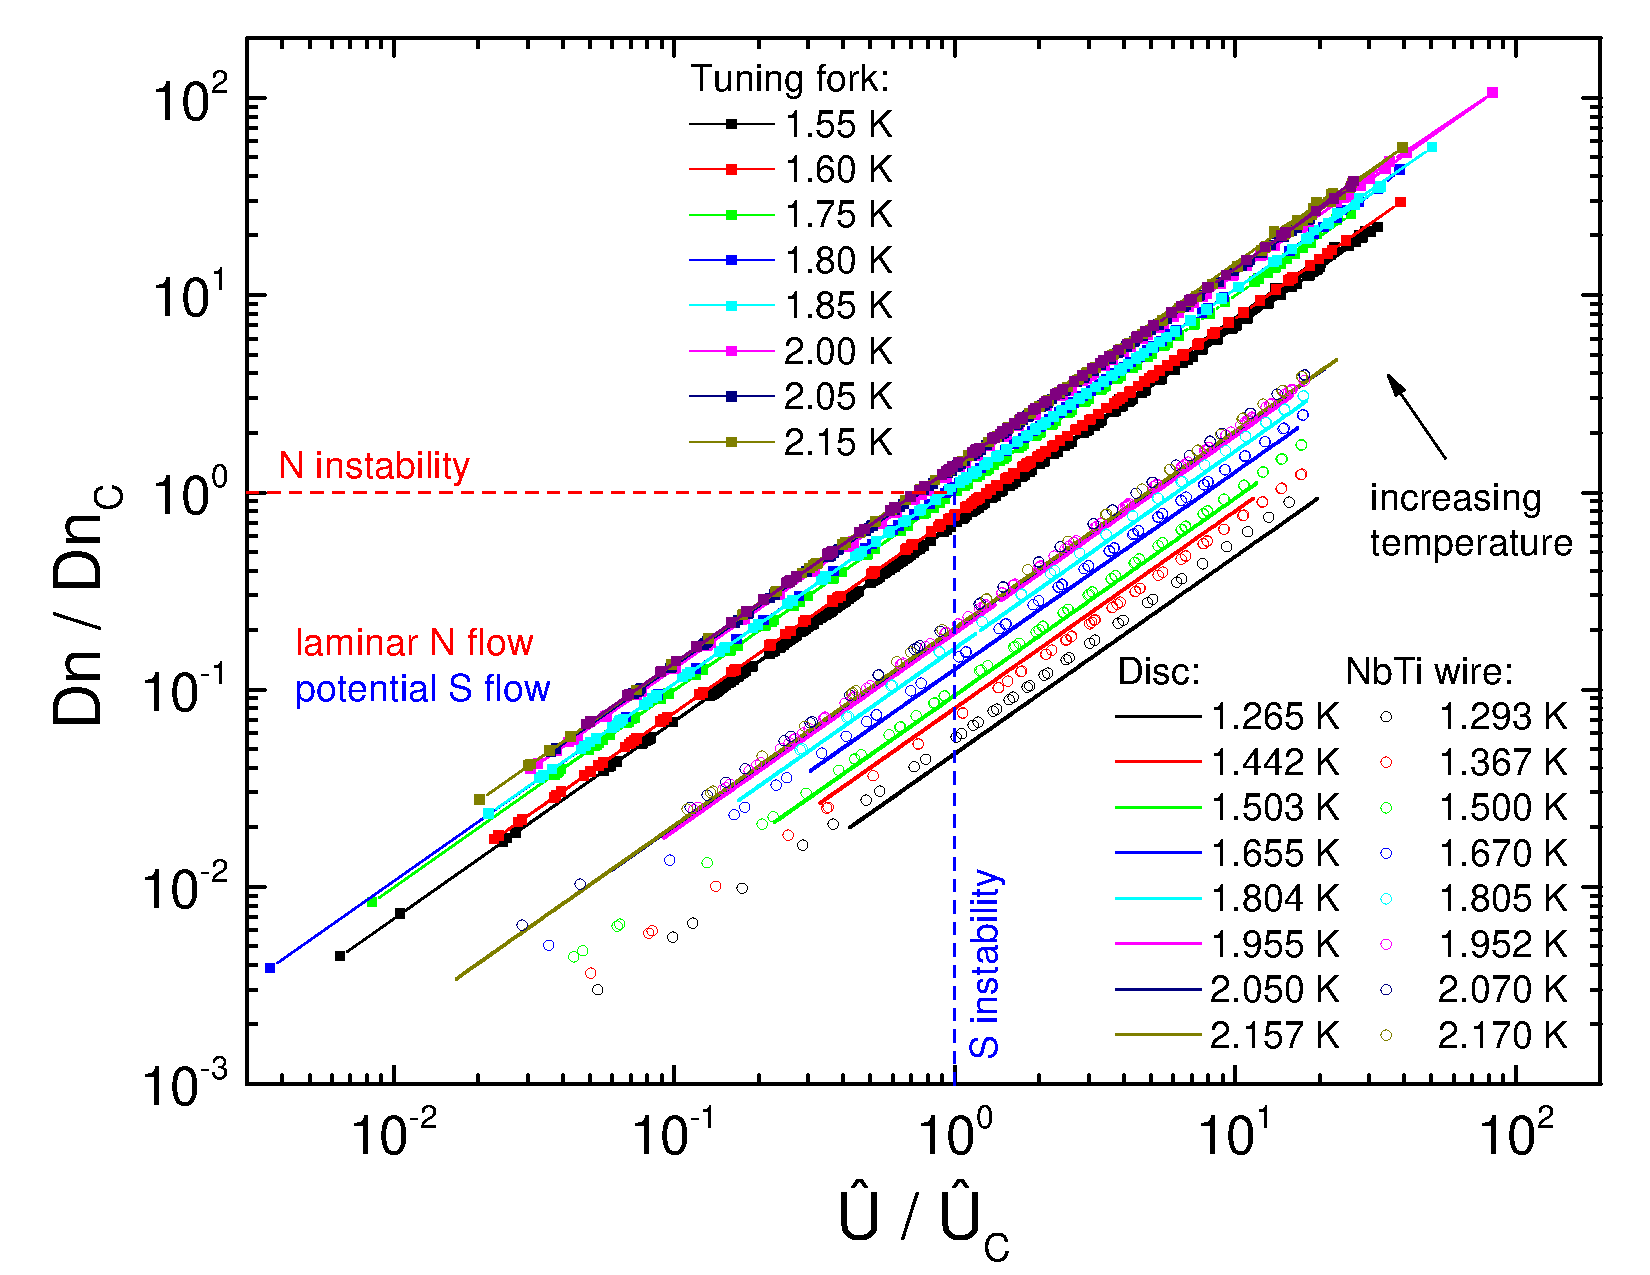
\includegraphics[width=0.8\textwidth]{graphics/results/flow_phase_diagram}
	\caption{Plot of Donnelly numbers against dimensionless velocities for three oscillators - vibrating wire, oscillating disc and tuning fork - submerged in Helium-II.\\
	\underline{Dashed lines} mark the estimated areas of transition from laminar/potential regimes to the non-linear ones, both for normal and superfluid components. The data used as a tuning fork is sourced from a different experiment, exhibiting the same behaviour.}
	\label{flow_phase_diagram}
\end{figure}

Vibrating wire and oscillating disc reach QT \underline{as the first transition}. From that, it is questionable when the CT was exactly triggerred since the exact bahaviour of QT evolution with oscillation velocity is not yet known. However, the tuning fork was the only oscillator that \underline{encountered the CT earlier than QT} for a certain tmeperatures $T \gtrsim 1.6\unit{K}$.\\
Which instability occurs as the first depedens both on geometry of the oscillator and temperature. Nevertheless, phase flow diagram proved itself as an useful visualisation for such purpose.

Additionally, we presented a formalism allowing the comparison between measurements in \underline{hydrodynamical} and \underline{non-newtonian} (thus ballistic) regimes of Helium-II. We have confirmed the universal scaling concept suggested for laminar flows in high-frequency limit, using the scaling function $f(\text{Wi})$.\\
However, the transitional flow regime ($\text{Wi} \sim 0.1$) reamins an open challenge to the theoretical and experimental investigation.


\section{Simulation conclusions}

We proposed an effective numerical method to compute the time evolution of vortex ring in superfluid He-II. All numerics is implemented in Python 3 and publicly uploaded on \href{https://github.com/KuboBahyl/superfluid}{GitHub} repository.\\
Performance of vortex filament model was improved by neglegcting the Biot-Savart integral, showing that the percentual errors are small, and updating the LIA calculation instead. Simulation well replicates the physical processes and performs with sufficient stability when using testing vortex ring of radius $R \in \langle 500, 2000 \rangle \mu\text{m}$ in resolution $\delta \in (60 - 100) \mu\text{m}$.


\newpage

%\chapter{Appendix}

To run the code, there has to be installed only Python 3 (with various libraries) on any OS. All the Python code can be found in the directory \texttt{src/}. The entire project is open-source and can be found as a public \href{https://github.com/KuboBahyl/superfluid}{GitHub} repository. Pull requests of any further development would be definitely appreciated.

Here we briefly present a few visualisations of observed instabilities and physical processes.

\subsection*{Instability in good resolution}


\begin{figure}[h]
	\centering
	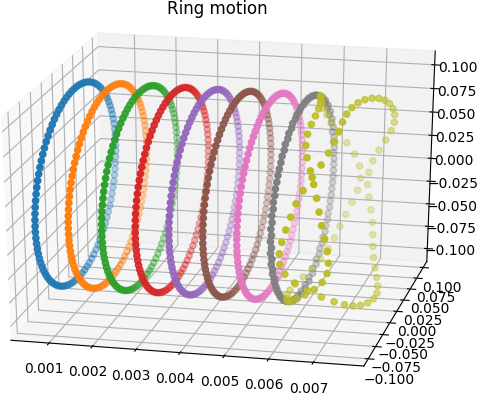
\includegraphics[width=0.6\textwidth]{graphics/results/euler_instability}
	\caption{A graphical example of ring instability when Euler stepping was used with good resolution (small $\delta$). Ring is moving from the left side to the right with exponentially forwarding error.}
\end{figure}

\subsection*{Noisy instability in worse resolution}

\begin{figure}[h]
	\centering
	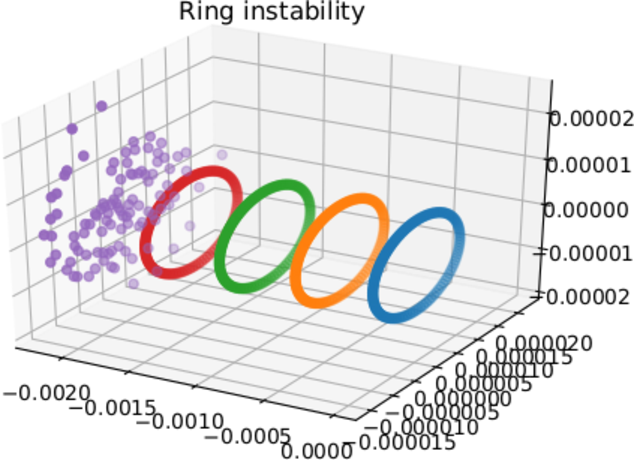
\includegraphics[width=0.6\textwidth]{graphics/results/ring-instability}
	\caption{Another example of ring instability due to forwarded numerical error using Euler stepping. In this case, resolution $\delta$ is higher (worse resolution), so the instability itself is much more noisy.}
\end{figure}

\newpage

\subsection*{Mutual frtiction effects}

Also, we present one of the bigger simulations (\textbf{Figure 17}) we tested. After we set the ring radius $R=1000\mu\text{m}$, resolution $\delta=60\mu\text{m}$ (resulting in around $\approx$ 100 mesh points),
re-segmentation boundaries $\delta_{\text{min}}= \delta /2 = 30\mu\text{m}$, $\delta_{\text{max}} = 2\delta = 120\mu\text{m}$, the updated LIA calculation, RK4 stepping method and a temperature $T=1.5\text{K}$, we obtained a stable simulation of vortex ring with a decreasing radius. More on particular physical processes can be found in \cite{biot_origin}.

\begin{figure}[h]
	\centering
	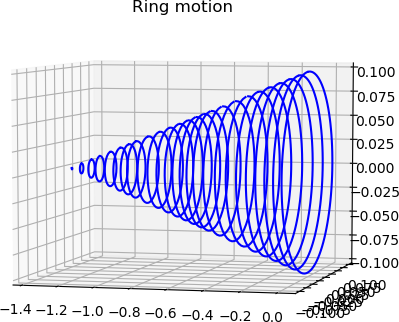
\includegraphics[width=0.6\textwidth]{graphics/results/ring-motion_full}
	\caption{Here, a vortex ring is moving to the left, its energy is dissipating due to the mutual friction and therefore, the radius is decreasing in time. The ring re-segmented itself a few times (due to the violation of $\delta_{\text{min}}$ condition and died (the simulation was stopped) when the length error was too high.}
\end{figure}

\newpage

% Norma citácii: ISO 690

\def\bibname{Bibliography}
\begin{thebibliography}{99}
	\addcontentsline{toc}{chapter}{\bibname}

	\bibitem{tisza}
	{\sc Tisza, L.}
	\emph{The viscosity of liquid helium and the Bose-Einstein statistics.}\\
	Comptes Rendus Acad. Sciences, \textbf{207}:1186-1189 (1952)

	\bibitem{landau}
	{\sc Landau, L.D.}
	\emph{The theory of superfluidity of helium II}\\
	J. Phys. USSR, Vol. \textbf{11}, 91 (1947)

	\bibitem{svoc2016}
	{\sc Bahyl, J.}
	\emph{Measurement of quantum turbulence in superfluid He-4}.
	Student conference, FMPH UK, Bratislava (2016)

	\bibitem{universal_scaling}
	{\sc Jackson, M.J., Schmoranzer, D., et al.}
	\emph{Universal Drag Force Scaling in High Stokes Number Oscillatory Flows of He II}. Phys Rev B, \textbf{submitted} (2018)

	\bibitem{vortex_ring}
	{\sc Rayfield, G.W., Reif F.}
	\emph{Quantized Vortex Rings in Superfluid Helium} Phys. Rev. A, \textbf{136}, 5A (1964)

	\bibitem{feynman}
	{\sc Feynman, R.}
	\emph{Application of quantum mechanics to liquid helium}.\\
	Prog. in Low Temp. Phys., \textbf{1}, 17-53 (1955)

	\bibitem{onsager}
	{\sc Penrose, O., Onsager, L.}
	\emph{Bose-Einstein condensation and liquid helium}.\\
	Phys. Rev., \textbf{104}, 576 (1956)

	\bibitem{vinen}
	{\sc Vinen, W.F.} and {\sc Hall, H.E.}
	\emph{The theory of mutual friction in uniformly rotating helium II}.
	Proc. Royal Soc. London 238 (1957) 204

	\bibitem{donnelly}
	{\sc Donnelly, R.J., Barenghi, C.F}
	\emph{The Observed Properties of Liquid Helium at the Saturated Vapor Pressure}. American Ins. of Phys. and Chem. Soc. (1998)

	\bibitem{roberts}
	{\sc Roberts, P.H.}
	\emph{} Phys. Rev. A, 55 (1971)

	\bibitem{donnelly_book}
	{\sc Donnelly, R.J.}
	\emph{Quantized Vortices in Helium II}.\\
	Cambridge studies in low temp. phys. (2005)

	\bibitem{osborne}
	{\sc Osborne, D.V.}
	\emph{The Rotation of Liquid Helium-II}.\\
	Proc. Royal Soc. London , \textbf{63}: 909-912 (1950)

	\bibitem{laminar-turbulence}
	{\sc Van Dyke, M.}
	\emph{An Album of Fluid Motion}.\\
	The Parabolic Press, Stanford, California (1982). ISBN 0-915760-02-9

	\bibitem{stokes}
	{\sc Schmoranzer, D., Kráľová, V., et al.}
	\emph{}	Phys. Rev. E, 81 (2010)

	\bibitem{crit-velocity}
	{\sc Nichol, H.A., Skrbek, L. et al.}
	\emph{} Phys. Rev. Lett. \textbf{92} (2004).

%%%%%%%%%%%%%%%%%%%%%%%%%%%%%%%%%%%%%%%%%%%%%%%%%%%%%%%%%%%%%%%%%

	\bibitem{skyba}
	{\sc Holt, S., Skyba, P.}
	\emph{} Rev. Sci. Instrum., \textbf{83} (2012)

	\bibitem{wire}
	{\sc Guénault, A.M., Kennedy, S.G., et al.}
	\emph{} J, of Low Temp Phys., \textbf{62} (1986)

	\bibitem{forks}
	{\sc Blaauwgeers, R. Blažková, M.} \text{and col.}
	\emph{Quartz tuning fork: Thermometer, Pressure- and Viscometer for Helium Liquids} J. of Low Temp Phys., Vol. \textbf{146} (2007)

	\bibitem{fork-exp}
	{\sc Bradley, D.I., Človečko, M.} \text{and col.}
	\emph{} Phys. Rev. B \textbf{85} (2012)

	\bibitem{multiple-vels}
	{\sc Schmoranzer, D., Jackson. M.J., et al.}
	\emph{Multiple critical velocities in oscillatory flow of superfluid $\He$ due to quartz tuning forks}.
	Phys. Rev. B \textbf{94} (2010)

	\bibitem{bakalaris}
	{\sc Bahyl, J.}
	\emph{Measurement of Quantum Turbulence in Superfluid Helium Using Second Sound Attenuation}.
	Bachelor Thesis, FMPH UK, Bratislava (2016)

%%%%%%%%%%%%%%%%%%%%%%%%%%%%%%%%%%%%%%%%%%%%%%%%%%%%%%%%%%%%%%%%%

	\bibitem{schwarz}
	{\sc Schwarz, K.W.}
	\emph{Three-dimensional vortex dynamics in superfuid He 4: Homogeneous superfluid turbulence}\\
	Phys Rev B, Vol. \textbf{38}, 4 (1988)

	\bibitem{tsubota}
	{\sc Tsubota, M., Fujimoto, K., Yui S.}
	\emph{Numerical Studies of Quantum Turbulence}.\\
	Journal of Low Temp Phys, 188 (2017)

	\bibitem{FDclosed}
	{\sc Baggaley, A.W., Barenghi, C.F.}
	\emph{Spectrum of turbulent Kelvin-waves cascade in superfluid helium}.\\
	Phys Rev B, Vol. \textbf{83}, 4 (2011)

	\bibitem{samuels}
	{\sc Samuels, D.C.}
	\emph{Superfluid vortices and Turbulence}. Quantized Vortex Dynamics and Superfluid Turbulence, Chap.9 (2001)

	\bibitem{barenghi}
	{\sc Barenghi, F.}
	\emph{Superfluid vortices and Turbulence}. Quantized Vortex Dynamics and Superfluid Turbulence, Chap.1 (2001)

	\bibitem{tree_alg}
	{\sc Baggaley, A.W., Barenghi, C.F.}
	\emph{Tree Method for Quantum Vortex Dynamics}. Journal of Low Temp Phys, 166 (2012)

	\bibitem{barnes}
	{\sc Barnes, J., Hut, P.}
	\emph{A hierarchical O(N log N) force-calculation algorithm}. Nature, \textbf{324}, 446 (1986)

	%%%%%%%%%%%%%%%%%%%%%%%%%%%%%%%%%%%%%%%%%%%%%%%%%%%%%%%%%%%%%%%%%



\end{thebibliography}



\end{document}
